\documentclass[14pt]{extarticle}
\usepackage[utf8]{inputenc}

\usepackage{algorithm}
\usepackage{algpseudocode}

\usepackage{algpseudocode}
\usepackage{geometry}
\geometry{
    a4paper,
    left=30mm,
    right=10mm,
    bottom=20mm,
    top=20mm
}
\linespread{1.5}

\usepackage[english, russian]{babel}
\usepackage{tempora}
\usepackage{soul, color}
\usepackage{newtxmath}
\usepackage{ragged2e}
\usepackage{xparse}
\usepackage{indentfirst}

\usepackage{subfigure}
\usepackage[]{graphicx}

\usepackage{amsmath}
\usepackage{booktabs}
\usepackage{multirow}

\usepackage{hyperref}

\let\openbox\relax
\usepackage{amsthm}



\begin{document}

    \include{macros}

    \begin{titlepage}

    \begin{center}
        ФЕДЕРАЛЬНОЕ  ГОСУДАРСТВЕННОЕ АВТОНОМНОЕ \\
        ОБРАЗОВАТЕЛЬНОЕ УЧРЕЖДЕНИЕ
        ВЫСШЕГО ОБРАЗОВАНИЯ
        «НАЦИОНАЛЬНЫЙ ИССЛЕДОВАТЕЛЬСКИЙ УНИВЕРСИТЕТ \\
        «ВЫСШАЯ ШКОЛА ЭКОНОМИКИ»
\\
\vspace{10mm}
        \textbf {
            Факультет информатики, математики и компьютерных наук \\
            Программа подготовки магистров по направлению \\
            01.04.02 Прикладная математика и информатика
        }
        \\
        \vspace{20mm}
        \textit{Трутнев Алексей Игоревич}
        \\
        \textbf{ВЫПУСКНАЯ КВАЛИФИКАЦИОННАЯ РАБОТА}
        \\
        \vspace{10mm}
        Кластеризация в пространствах большой размерности
        \vspace{10mm}
    \end{center}

\vspace{50mm}

\hfill
\begin{minipage}{0.4\textwidth}
    \begin{flushleft}
        Рецензент \\
        инженер-исследователь компании Хуавей \\
        \signatureline[6cm]{}
        \\
        М.А. Казаков
    \end{flushleft}
\end{minipage}
\hfill
\begin{minipage}{0.4\textwidth}
    \begin{flushright}
        Научный руководитель \\
        д-р физико-математических наук, проф. \\
        \signatureline[6cm]{}
        \\
        В.А. Калягин
    \end{flushright}
\end{minipage}

\begin{center}
    \vspace*{\fill}
    Нижний Новгород, 2025
\end{center}

\end{titlepage}
    \setcounter{page}{2}

    \tableofcontents

    % \section{Введение}

Кластеризация является важным инструментом анализа данных, который находит широкое применение во многих областях, включая биоинформатику, медицину, финансы, исследования социальных сетей и многие другие. Однако с увеличением размерности данных стандартные методы кластеризации могут столкнуться с проблемой низкого качества разбиения.

Проблема качества кластеризации особенно остра в многомерном пространстве, где количество признаков значительно превышает количество объектов. Это явление, известное как <<проклятие размерности>>, приводит к тому, что традиционные методы кластеризации становятся менее эффективными из-за разреженности данных и трудностей в интерпретации результатов.

Одним из способов преодоления этой проблемы является привлечение учителя для предоставления дополнительной информации о данных. Однако разметка больших наборов данных для обучения моделей машинного обучения с учителем требует значительных временных и финансовых затрат. В связи с этим возникает потребность в разработке методов кластеризации, которые могли бы использовать только часть размеченных данных для улучшения качества разбиения.

В данной работе исследуется подход кластеризации с частичным привлечением учителя (\ssClustering{}), который позволяет использовать ограниченное количество размеченных данных для повышения эффективности кластеризации в пространствах большой размерности.

Для достижения данной цели поставлены следующие задачи:
\begin{enumerate}
\item систематизировать и проанализировать существующие методы кластеризации,
\item реализовать алгоритм кластеризации с частичным привлечением учителя в пространствах большой размерности,
\item провести экспериментальное исследование и анализ влияния параметров алгоритма на качество кластеризации.
\end{enumerate}

В результате выполнения поставленных задач будет разработан новый метод кластеризации с частичным привлечением учителя. Особенностью предложенного метода является его способность эффективно работать с ограниченным объемом размеченных данных, что делает его особенно привлекательным для сфер, где разметка данных является сложной, трудоемкой и дорогостоящей задачей, включая анализ текста, аудиосигналов изображений и других.
Кроме того, данная работа предоставит возможность глубже исследовать и понять, как ограниченный объем размеченных данных может быть использован для улучшения качества кластеризации. Это позволит существенно оптимизировать процесс разметки данных и снизить затраты на него.


    % \section{Обзор литературы}

    \subsection{Введение в кластеризацию}

        Кластеризация представляет собой один из фундаментальных методов машинного обучения, используемый для группировки объектов на основе их внутренних признаков и сходства без привлечения учителя, то есть без использования размеченных данных. В отличие от классификации, где объекты распределяются по заранее определенным классам, кластеризация позволяет выявлять скрытые структуры и закономерности в данных, что делает ее особенно полезной в ситуациях, когда заранее неизвестно, как должны выглядеть классы или группы.

        Кластеризация применяется в широком спектре научных и прикладных задач, охватывая такие области, как анализ данных \cite{SETYANINGSIH2012286}, компьютерное зрение \cite{Demidovskij2023ids}, биоинформатика \cite{Kiselev2019scRNAseqClustering}, обработка естественного языка \cite{Grootendorst2022BERTopic}, а также информационные технологии, социальные науки, медицина и финансовая аналитика. Ее основная цель -- разделить множество объектов на группы (кластеры) таким образом, чтобы объекты в пределах одного кластера обладали максимальной степенью сходства, в то время как объекты различных кластеров были существенно различны.

        Кластеризация может быть использована для решения различных задач, таких как:
        \begin{itemize}
            \item \textbf{Сегментация изображений}: разделение изображения на области схожих пикселей, что позволяет выделить объекты на изображении и улучшить качество последующего анализа.
            \item \textbf{Классификация текстов}: группировка текстовых документов по темам или стилям, что позволяет упростить поиск и анализ информации.
            \item \textbf{Кластеризация пользователей}: сегментация пользователей на группы схожих интересов и предпочтений, что позволяет персонализировать рекомендации и маркетинговые стратегии.
            \item \textbf{Обнаружение аномалий}: выявление аномальных точек, не принадлежащих ни одному кластеру или попадающих в редкие группы, что может свидетельствовать о мошенничестве, сбоях в оборудовании или ошибках в данных.
            \item \textbf{Разведочный анализ данных (EDA, Exploratory Data Analysis)}: выявление скрытых закономерностей и структур в данных, что особенно полезно при работе с новыми или плохо изученными наборами данных.
        \end{itemize}

    \subsection{Методы кластеризации}
        Существуют различные подходы к реализации кластеризации, отличающиеся не только алгоритмической природой, но и способностью справляться с различными типами данных и структурами кластеров. В зависимости от метода формирования кластеров можно выделить следующие основные категории:

        \begin{itemize}
            \item \textbf{Центроидные методы} -- основаны на минимизации расстояний между объектами и центроидами (центральными точками) кластеров (\kmeans{}, \kmedoids{}).
            \item \textbf{Иерархические методы} -- формируют древовидную структуру кластеров путем последовательного объединения или разбиения групп (агломерационная и дивизионная кластеризация).
            \item \textbf{Плотностные методы} -- строят кластеры как области повышенной плотности объектов (например, DBSCAN, OPTICS).
            \item \textbf{Модельные методы} -- предполагают, что данные генерируются из смеси вероятностных распределений (например, EM-алгоритм для гауссовых смесей).
            \item \textbf{Спектральные и графовые методы} -- используют спектральные свойства графов и матриц смежности для обнаружения кластеров в данных со сложной топологией.
        \end{itemize}

        Каждый из подходов обладает своими достоинствами и ограничениями, что требует осознанного выбора метода в зависимости от конкретных характеристик исследуемых данных: размерности, плотности, формы кластеров и наличия шумов.

        \subsubsection{Кластеризация на основе центроидов}

            Кластеризация на основе центроидов (centroid-based clustering) представляет собой один из наиболее интуитивно понятных и широко используемых подходов к группировке данных. Суть данного метода заключается в том, что каждый кластер описывается так называемым центроидом -- обобщенным представлением <<центра тяжести>> данных в пределах соответствующего кластера. Объекты присваиваются к тому или иному кластеру на основе минимизации расстояния до соответствующего центроида.

            Наиболее известным и базовым представителем  кластеризации на основе центроидов является алгоритм \kmeans{} \cite{Lloyd1982kmeans}. Данный алгоритм итеративно обновляет позиции центроидов и перераспределяет объекты между кластерами с целью минимизации инерции -- суммарного квадратичного расстояния между объектами и центрами кластеров. Простота реализации и высокая вычислительная эффективность обеспечили \kmeans{} широкое распространение, особенно при работе с большими объемами данных.

            Однако классический \kmeans{} обладает рядом существенных ограничений. Во-первых, он чувствителен к начальной инициализации центроидов, что может приводить к сходимости к локальным минимумам. Во-вторых, алгоритм предполагает заданное заранее число кластеров \(k\), что не всегда возможно определить. Кроме того, алгоритм плохо справляется с кластерами, имеющими сложную форму, различную плотность или отличающиеся размерами.

            В ответ на указанные ограничения было предложено несколько модификаций. Один из таких подходов -- \kmeans{}++ \cite{Arthur2010kmeans++}, который улучшает этап начальной инициализации центроидов путем применения стохастической стратегии выбора начальных точек. Это повышает стабильность и качество итогового разбиения, особенно при наличии шумов и неоднородности в данных.

            Альтернативой, сохраняющей идею центроидного представления, является алгоритм \kmedoids{}, также известный как PAM (Partitioning Around Medoids) \cite{kaufman2008kmedioids}. В отличие от \kmeans{}, где центроиды могут быть абстрактными точками, \kmedoids{} использует в качестве центров реальные объекты из выборки -- медианы. Это повышает устойчивость к выбросам и позволяет использовать произвольные метрики расстояния, включая манхэттенскую, косинусную и другие, однако вычислительная сложность алгоритма существенно выше, особенно при больших объемах данных.

            Среди более современных подходов можно выделить CLARANS (Clustering Large Applications based upon RANdomized Search) \cite{Ng1994clarans}, который комбинирует элементы \kmedoids{} с методами стохастического поиска и улучшает масштабируемость алгоритма при работе с крупными выборками. В свою очередь, Mini-Batch \kmeans{} \cite{Sculley2010minibatch} адаптирован для обработки потоков данных и масштабных задач за счет обновления центроидов на основе случайных подвыборок (батчей), что уменьшает требования к памяти и ускоряет обучение.

            Несмотря на ограниченность в обнаружении кластеров сложной формы, методы, основанные на центроидах, остаются актуальными благодаря своей простоте, интерпретируемости и высокой вычислительной эффективности. Они особенно полезны в качестве базовых моделей или в составе более сложных гибридных решений, где предварительная кластеризация используется как этап инициализации или предобработки данных.

        \subsubsection{Кластеризация на основе плотности}

            Методы кластеризации на основе плотности (density-based clustering) представляют собой эффективный класс алгоритмов, разработанных для выявления кластеров в данных с неоднородной плотностью распределения. Основная идея заключается в том, что кластеры формируются как связные области пространства с высокой плотностью объектов, отделенные друг от друга зонами разреженности. В отличие от методов, основанных на центроидах или иерархической структуре, плотностные алгоритмы способны выделять кластеры произвольной формы, устойчивы к шуму и выбросам, а также не требуют предварительного задания числа кластеров.

            Наиболее известным и фундаментальным методом в этой категории является DBSCAN (Density-Based Spatial Clustering of Applications with Noise) \cite{Ester1996DBSCAN}. Алгоритм определяет кластеры как максимальные области, содержащие взаимосвязанные точки с плотностью выше заданного порога. Основные параметрами алгоритма радиус окрестности и минимальное число точек в окрестности позволяют определить является ли точка ядровой, граничной или шумовой. DBSCAN эффективно справляется с задачами обнаружения кластеров различных форм, но его производительность существенно зависит от корректного выбора параметров, что особенно проблематично при переменной плотности данных.

            Для преодоления ограничений DBSCAN в условиях разной плотности кластеров был предложен алгоритм OPTICS (Ordering Points To Identify the Clustering Structure) \cite{Ankerst1999OPTICS}. В отличие от DBSCAN, OPTICS не производит окончательное разбиение, а строит упорядоченное представление плотности данных, называемое reachability plot. Это позволяет визуально определить плотностные структуры и формировать кластеры постфактум, адаптируясь к локальным особенностям плотности. OPTICS расширяет применимость методов плотностной кластеризации, особенно в случаях с вложенными и слабо выраженными структурами.

            Более современным и мощным развитием идей DBSCAN является HDBSCAN (Hierarchical DBSCAN) \cite{Maarten2022HDBSCAN}. Данный алгоритм строит иерархическую дендрограмму на основе плотностной связи между точками, а затем применяет процедуру извлечения стабильных кластеров. Он автоматически определяет оптимальное количество кластеров и значительно лучше справляется с кластерами переменной плотности, при этом наследуя устойчивость DBSCAN к шуму. HDBSCAN также предлагает оценку надежности принадлежности точки к кластеру, что повышает интерпретируемость результатов.

            Другим интересным направлением является DENCLUE \cite{DENCLUE}, использующий ядерные оценки плотности (kernel density estimation) для моделирования распределения данных. Это позволяет формировать кластеры на основе градиентных потоков в плотностном пространстве и обеспечивает гибкую настройку формы и гладкости кластеров. Однако метод требует вычислительно дорогих операций и чувствителен к выбору параметра сглаживания.

            Плотностные алгоритмы находят широкое применение в задачах обнаружения аномалий, анализе геопространственных данных, выявлении сообществ в социальных сетях и анализе временных рядов, где традиционные методы центроидного типа или иерархические подходы оказываются неэффективными.

            В целом, подходы, основанные на плотности, являются мощными средствами анализа сложных, неструктурированных и шумных данных. Их гибкость и устойчивость делают их незаменимыми в случаях, когда структура кластеров заранее неизвестна и может отличаться высокой степенью нелинейности.

        \subsubsection{Иерархическая кластеризация}
            Иерархическая кластеризация представляет собой мощный класс алгоритмов, ориентированных на поэтапное построение структуры вложенных кластеров без необходимости заранее задавать их количество. В отличие от центроидных и плотностных методов, иерархический подход формирует древовидную структуру, называемую дендрограммой, где каждый уровень отражает определенный этап объединения или разбиения кластеров. Это делает метод особенно полезным для визуального анализа структуры данных и выбора оптимального количества кластеров после завершения обучения.

            Существует два основных направления иерархической кластеризации:

            \begin{itemize}
                \item Агломеративная стратегия, при которой каждый объект изначально рассматривается как отдельный кластер, и далее происходит последовательное объединение ближайших кластеров вплоть до образования единой группы. Данный подход является наиболее распространенным и практически применимым, особенно в случае умеренных размеров выборки. Одним из самых популярных алгоритмов этой категории является метод Уорда \cite{Murtagh2011wardalgo}, минимизирующий увеличение внутрикластерной дисперсии при каждом объединении.
                \item Дивизионная стратегия, напротив, начинается с единственного кластера, включающего все объекты, и рекурсивно разделяет его на подмножества. Несмотря на высокую концептуальную привлекательность, методы этого типа требуют значительно больших вычислительных затрат и применяются реже \cite{Kaufman1990divisive}.
            \end{itemize}

            Качество работы иерархической кластеризации в значительной степени зависит от выбора метрики расстояния между кластерами. Существует несколько стратегий, определяющих, как именно измеряется расстояние между группами данных:

        \paragraph{Single Linkage (Метод ближнего соседа)}
            Метод ближнего соседа \cite{Sibson1973SLINK} определяет расстояние между кластерами как минимальное расстояние между парой точек из разных кластеров. Он хорошо справляется с кластеризацией вытянутых или нестандартных форм, однако чувствителен к шуму и может приводить к так называемому «эффекту цепочки» -- последовательному объединению разреженных объектов.

        \paragraph{Complete Linkage (Метод дальнего соседа)}
            В методе дальнего соседа \cite{Defays1977CLINK} расстояние между кластерами определяется как максимальное расстояние между точками двух кластеров. Этот подход обеспечивает более компактные и равномерные кластеры, но при этом склонен переоценивать расстояния и может неправомерно разделять вытянутые структуры.

        \paragraph{Average Linkage (Метод средней связи)}
            Средняя связь \cite{Finkelman2021averagelinkage} использует среднее значение расстояний между всеми парами точек из двух кластеров. Данный метод обеспечивает баланс между крайними подходами и демонстрирует устойчивость к шуму, но иногда недостаточно точно отражает геометрию данных.

        Кроме того, иерархические методы удобны тем, что позволяют динамически выбирать оптимальное число кластеров, обрезая дендрограмму на нужной высоте без необходимости многократного запуска алгоритма. Это особенно ценно в условиях, когда структура данных неизвестна заранее.

        Несмотря на высокую интерпретируемость и визуальную наглядность, недостатками иерархических методов являются высокая вычислительная сложность ( \(\mathcal{O}(n^2)\) или выше для большинства реализаций) и невозможность коррекции ошибок: однажды принятые решения о слиянии или разбиении не подлежат пересмотру.

        Тем не менее, иерархическая кластеризация остается важным инструментом в арсенале анализа данных и активно применяется в биоинформатике, текстовом анализе, социологии, психологии и других дисциплинах, где требуется исследование сложных иерархических структур в выборке.

    \subsubsection{Кластеризация на основе обучения Хебба}
        Кластеризация на основе обучения Хебба (Hebbian Learning) представляет биологически вдохновленный метод обучения, основывающийся на фундаментальном принципе нейрофизиологии. Согласно так называемому правилу Хебба \cite{Hebb1949}, «нейроны, которые активируются совместно, укрепляют связь между собой» (neurons that fire together, wire together). Эта идея легла в основу адаптивного обучения в искусственных нейронных сетях, а также стала мощным инструментом для кластеризации данных на основе корреляционной близости объектов.

        С точки зрения формализации, классическое обучение по правилу Хебба предполагает обновление весов связей по правилу:
        \begin{equation}
            \Delta w = \eta x y,
        \end{equation}
        где \(x\) и \(y\) -- входной и выходной сигналы, \(w\) -- вес связи между входом и выходом, а \(\eta\) -- коэффициент обучения. При многократном предъявлении данных такие схемы обучения приводят к усилению связей между часто совместно активируемыми признаками, что способствует формированию естественных кластеров.

        Преимуществом данного метода кластеризации является биологическая правдоподобность, адаптивность к данным, способность выявлять латентные структуры без строгих априорных предположений о количестве кластеров. Однако они также обладают определенными ограничениями. Наиболее существенными из них являются чувствительность к параметру обучения и зависимость от порядка предъявления входов.

        Тем не менее, обучение по правилу Хебба продолжает рассматриваться как перспективная альтернатива классическим методам кластеризации, особенно в условиях отсутствия четких границ между группами данных.


    \subsection{Проблемы пространства большой размерности}
        Анализ и кластеризация данных в пространствах высокой размерности остаются актуальными задачами современной науки о данных. По мере увеличения числа признаков (измерений), используемых для описания объектов, традиционные методы анализа, включая алгоритмы кластеризации, начинают сталкиваться с фундаментальными затруднениями. Это явление широко известно как <<проклятие размерности>> (curse of dimensionality) \cite{Bellman1957cursedim}.

        \paragraph{Вычислительная сложность}
            Одним из наиболее очевидных последствий высокой размерности является экспоненциальный рост вычислительной нагрузки. Многие алгоритмы кластеризации, в частности \kmeans{}, требуют вычисления расстояний между каждым объектом и каждым центроидом на каждой итерации. При этом сложность возрастает линейно по числу измерений и квадратично по числу объектов. В пространствах с тысячами признаков это приводит к существенному увеличению времени работы алгоритмов и ресурсов памяти, ограничивая масштабируемость \cite{Verleysen2005curse}.

        \paragraph{Разреженность данных}
            По мере увеличения размерности пространства наблюдается феномен разреженности -- объекты становятся статистически эквивалентно удаленными друг от друга, и плотность данных резко падает. Как показано в \cite{Beyer1999NearestNeighbor}, различия в расстояниях между ближайшими и дальними соседями стремятся к нулю по мере роста размерности, делая евклидову метрику все менее информативной \cite{aggarwal2001surprising}. Это приводит к затруднениям в определении границ между кластерами, особенно при использовании методов на основе расстояния и плотности (например, \kmeans{}, DBSCAN).

    \subsubsection{Использование расстояния Минковского}
        Одной из возможных стратегий повышения качества кластеризации в пространствах большой размерности является адаптация метрики расстояния. В этом контексте особое внимание заслуживает расстояние Минковского, которое представляет собой обобщение различных метрических функций:
        \begin{equation}
            \label{eq:minkowski}
            d(x, y) = \left( \sum_{i=1}^{n} |x_i - y_i|^p \right)^\frac{1}{p}.
        \end{equation}
        Значения параметра \(p\) позволяют интерполировать между манхэттенской (\(p=1\)) и евклидовой (\(p=2\)) метриками, а при \(p \to \infty\) метрика приближается к максимуму по координатам. Исследования показали, что выбор оптимального значения параметра \(p\) может существенно повлиять на эффективность кластеризации в условиях высокой размерности \cite{aggarwal2001surprising}. Особенно перспективным направлением является использование взвешенного расстояния Минковского, где каждый признак имеет индивидуальный вес:
        \begin{equation}
            \label{eq:weighted_minkowski}
            d(x, y) = \left( \sum_{i=1}^{n} w_i |x_i - y_i|^p \right)^\frac{1}{p},
        \end{equation}
        где \(w_i\) -- вес признака \(i\). Эти веса могут быть получены, например, с помощью анализа важности признаков, извлеченной из моделей машинного обучения, либо с использованием разложения главных компонент (PCA). Такой подход позволяет учитывать разную информативность признаков, что особенно важно в условиях высокой размерности и коррелированных признаков. Практические результаты подтверждают, что взвешенные метрики существенно улучшают устойчивость алгоритмов, таких как \kmeans{}, к шуму и нерелевантным признакам \cite{chouikhi2015featureweighting}.

    \subsubsection{Кластеризация с частичным привлечением учителя}
        Другая важная стратегия повышения эффективности кластеризации -- это частичное привлечение учителя (semi-supervised clustering). Данная стратегия сочетает преимущества обучаемых без учителя методов с ограниченным числом меток классов, что позволяет направлять процесс кластеризации к более интерпретируемым и структурированным результатам. Такой подход используется, например, при наличии  информации о небольшом числе объектов, чья принадлежность к кластерам заранее известна, что позволяет добавить контроль в процесс кластеризации, приводя к созданию различимых кластеров с более четкой структурой, а также добавляя возможность использовать стандартные методы оценки качества результатов алгоритма, такие как точность (Accuracy), прецизионность (Precision) полнота (Recall). Среди алгоритмов кластеризации с частичным привлечением учителя можно выделить основные подходы использования ограниченного знания о классах исходных данных \cite{hse:5_course}.

        \paragraph{Привлечение учителя для генерации начальных кластеров}
            Подход кластеризации с частичным привлечением учителя для генерации начального разбиения на кластеры (seeding) \cite{basu2002seeding}, \cite{antoine2014seeding} -- это направление, в котором небольшой набор маркированных точек данных используют для формирования начальных кластеров, таким образом предоставляя алгоритму хорошую стартовую точку для оптимизационной задачи. В дальнейшем алгоритм кластеризации уже без учителя распространит начальные метки на оставшиеся немаркированные данные на основе мер схожести, обеспечивая сильное влияние начального приближения на весь процесс обучения.

        \paragraph{Привлечение учителя для определения принадлежности к кластеру}
            Одним из способов внести знания о кластерах в процесс обучения также является привлечение учителя для определения принадлежности к кластеру. Метод Semi-supervised clustering under a <<compact-cluster>> assumption \cite{jiang2023compactcluster}, который основан на допущении идеи компактности кластеров и минимизирует внутрикластерные расстояния, одновременно максимизируя межкластерные расстояния, обеспечивает четкость и компактность кластеров.

    \subsubsection{Self-Supervised Clustering}
        Самоконтролируемая кластеризация (Self-Supervised Clustering, SSL) представляет собой гибридную парадигму, сочетающую принципы самоконтролируемого обучения (Self-Supervised Clustering) с задачей кластеризации. В ее основе лежит идея извлечения устойчивых и структурно значимых признаков из неразмеченных данных, которые в дальнейшем могут использоваться для формирования кластеров с высокой интерпретируемостью и разделимостью. SSL зарекомендовал себя как эффективный инструмент предварительного анализа, способный существенно улучшать производительность задач, включая кластеризацию \cite{Gui2023SSL}.

        SSL представляет собой класс методов, в которых обучающая информация извлекается из самих данных без использования явных меток. В результате обучения создаются эмбеддинги (embeddings) -- векторы признаков, которые можно использовать в задачах сегментации, визуализации и кластеризации.

        Таким образом, SSL становится этапом предварительного анализа данных. Одним из таких методов может быть этап снижения размерности, позволяющий компактно представить данные в пространстве с меньшей размерностью, сохранив при этом ключевую топологическую структуру.

    \subsubsection{Методы снижения размерности}

        \paragraph{Метод главных компонент (Principal Component Analysis)}
            Метод главных компонент (PCA) -- это один из наиболее известных и широко используемых алгоритмов снижения размерности \cite{Jolliffe1986pca}. PCA позволяет перевести данные из пространства высокой размерности в подпространство меньшей размерности, сохранив при этом максимум возможной дисперсии данных. Важной особенностью метода является его линейная природа, что делает его особенно эффективным для задач, в которых основная информация содержится в линейных комбинациях признаков. Простота PCA, его высокая вычислительная эффективность и математическая интерпретируемость сделали метод фундаментальным инструментом в таких областях, как:
            \begin{itemize}
                \item обработка изображений (например, сжатие изображений, распознавание лиц \cite{Turk1991faces}),
                \item биоинформатика (анализ экспрессии генов \cite{Ringner2008pca}),
                \item финансовое моделирование (анализ корреляционных структур рынков),
                \item кластеризация и визуализация многомерных данных \cite{Jolliffe2016PCAbook}.
            \end{itemize}
            Однако, несмотря на достоинства, линейность PCA является его ограничением: метод не способен корректно обрабатывать данные, в которых основная структура отражается в нелинейных зависимостях между признаками.

        \paragraph{Метод многомерного шкалирования (Multidimensional Scaling)}
            Метод многомерного шкалирования (MDS) -- это классический подход к снижению размерности, направленный на сохранение попарных расстояний или близостей между объектами при отображении их в пространство меньшей размерности. В отличие от метода главных компонент (PCA), MDS может использовать любой тип метрик, включая неевклидовы, и поэтому считается более гибким для анализа данных с нелинейной структурой.

            MDS был впервые разработан как способ визуализации психологической близости между объектами на основе субъективных оценок \cite{Kruskal1964mds}. Позднее метод получил широкое распространение в информационных науках, биоинформатике, социальной аналитике, анализе текстов и других дисциплинах, где структура данных может быть выражена через матрицу попарных расстояний.

        \paragraph{Метод Uniform Manifold Approximation and Projection (UMAP)}
            Метод UMAP \cite{McInnes2018UMAP} представляет собой современный и эффективный нелинейный алгоритм снижения размерности, ориентированный на сохранение локальной и глобальной структуры данных. В отличие от классических линейных методов (например, PCA), UMAP обладает высокой масштабируемостью, вычислительной эффективностью и устойчивостью к шуму, что делает его востребованным в задачах визуализации, кластеризации и предварительной обработки данных.

        \paragraph{Метод Isometric Mapping (ISOMAP)}
            Метод ISOMAP -- это нелинейный алгоритм снижения размерности \cite{Tenenbaum2000isomap}, расширяющий классический метод многомерного шкалирования (MDS) и сохраняющий геодезические расстояния между точками, а не только их евклидову дистанцию. ISOMAP позволяет эффективно обрабатывать данные с нелинейной структурой, сохраняя при этом важные топологические свойства. Однако метод требует значительных вычислительных ресурсов и может быть чувствителен к шуму в данных.

        \paragraph{Метод Locally Linear Embeddings (LLE)}
            Метод LLE -- это эффективный алгоритм нелинейного снижения размерности \cite{Roweis2000LLE}, позволяющий получить компактное представление высокоразмерных данных, сохранив при этом локальную геометрию исходного пространства. В отличие от линейных методов, таких как PCA, LLE способен выявлять нелинейные структуры, что делает его особенно полезным для обработки данных, лежащих на искривленных многообразиях.

        \paragraph{Метод Spectral Embeddings (SSE)}
            Метод SSE, также известный как спектральное разложение графа или Laplacian Eigenmaps, представляет собой мощный инструмент нелинейного снижения размерности \cite{Belkin2001laplacian}. SSE опирается на представление данных в виде графа, в котором вершины соответствуют объектам, а ребра -- их близости. Метод позволяет сохранить локальную геометрию данных, что делает его особенно эффективным для задач, связанных с визуализацией, сегментацией и кластеризацией структурно сложных данных.

    \subsection{Выводы}
        В ходе проведенного обзора были рассмотрены основные алгоритмы кластеризации, применяемые в задачах анализа многомерных данных. Одной из ключевых проблем, выявленных при этом, стало существенное снижение качества кластеризации в условиях высокой размерности данных. Такая ситуация, характерная для многих современных наборов данных, приводит к явлению при котором традиционные алгоритмы, включая \kmeans{}, демонстрируют нестабильность и низкую точность результатов.
        Для преодоления этих ограничений активно применяются различные стратегии предварительной обработки данных, ключевую роль среди которых играет снижение размерности. Данный подход позволяет не только сократить вычислительную сложность алгоритмов, но и повысить устойчивость и точность кластеризации за счет устранения шумовых и коррелированных признаков.
        Несмотря на разнообразие существующих методов снижения размерности, на практике остается ряд открытых проблем. Во-первых, не существует универсального критерия выбора метода снижения размерности для конкретной задачи кластеризации. Во-вторых, влияние предварительного снижения размерности на итоговое качество кластеризации далеко не всегда очевидно и требует тщательного эмпирического анализа.


    % \section{Постановка проблемы}

\subsection{Основные обозначения}
В дальнейшем будут использоваться следующие основные обозначения. Пусть $X = \left( x_i^j \right) \in \mathbb{R}^{n \times d}$ обозначает матрицу наблюдений размером $n \times d$, где каждый $d$-мерный объект $x_i = (x_i^1, x_i^2, \dots, x_i^d) \in \mathbb{R}^{1 \times d}$ представляет собой строковый вектор признаков для каждого наблюдения $i=1,2,\dots,n$. Вектор $x_j = (x_1^j, x_2^j, \dots, x_n^j)^\top \in \mathbb{R}^{n \times 1}$ означает столбец значений признака $j$ для всех наблюдений $j=1,2,\dots,d$. Вектор $y = (y_1, y_2, \dots, y_n)^\top \in \mathbb{R}^{n \times 1}$ содержит значения целевой функции, представляющей искомые кластеры. Число кластеров обозначено как $k$, а разбиение наблюдений на кластеры — как $S={S_1, S_2, \dots, S_k}$, где каждый кластер $S_l \subset {1,2, \dots, n }$ для $l=1,2,\dots,k$. Набор из $k$ центров кластеров представлен через $c = { c_1,c_2, \dots, c_k }$, где каждый центр $c_l = (c_l^1, c_l^2, \dots, c_l^d) \in \mathbb{R}^{1 \times d}$ для $l=1,2,\dots,k$. Также используется диагональная матрица размерности $d$, обозначенная как $I_d$.


\subsection{Формулирование задачи кластеризации без учителя}
Задача кластеризации относится к типу задач <<без учителя>> (Unsupervised learning). Задача кластеризации -- есть группировка объектов в наборы (группы), основываясь только на их сходстве между собой так, чтобы объекты внутри одной группы были больше похожи на представителей этой группы, чем другой.

Формальная запись задач имеет следующий вид:
Для каждого $d$-мерного объекта $x_i$ из множества объектов $X = {x_1, x_2, ..., x_n}$, необходимо поставить в соответствие один из $k$ кластеров $c= \{c_1, c_2, \dots, c_k\}$.

Для оценивания <<схожести>> объектов могут быть использованы разные метрики расстояния такие как Евклидово расстояние \cite{Lloyd1982kmeans}, Манхеттенское расстояние, \cite{kaufman2008kmedioids}, расстояние Минковского \cite{aggarwal2001surprising} и другие. А также различные способы оценки межкласторных расстояний, такие как Average Linkage \cite{Finkelman2021averagelinkage}, Complete Linkage \cite{Defays1977CLINK}, Single Linkage \cite{Sibson1973SLINK}.


Задача кластеризации на основе центроидов для расстояния Минковского с параметром \(p\) есть задача сложной невыпуклой оптимизации функционала качества (\ref{eq:kmeans_problem}), которая может быть решена с помощью эвристического алгоритма \kmeans{} для метрики Минковского, где необходимо оптимизировать сумму расстояний между объектами внутри кластеров.

\begin{equation}
    \begin{gathered}
        W_p(S;c) = \sum_{l=1}^k \sum_{x \in S_l} \sum_{j=1}^{d} |x^j - c_l^j|^p \to \min, \\
        x=(x^1, x^2, \dots, x^d) \in R^{1 \times d}, \\
        c_l=(c_l^1,c_l^2, \dots, c_l^d) \in R^{1 \times d}
    \end{gathered}
    \label{eq:kmeans_problem}
\end{equation}

\subsubsection{Выбор метода кластеризации}

В данной работе основой для алгоритма кластеризации с учителем служит реализация \kmeans{} с метрикой Минковского для пространств большой размерности, поскольку \kmeans{} -- легко интерпретируемый подход, основанный на оптимизации суммарного квадратичного отклонения внутри кластеров. Выбор \kmeans{} также обусловлен его основными преимуществами: простотой реализации (существует большое число реализаций и оптимизаций данного подхода), высокой скоростью работы (на небольших наборах данных алгоритм способен сходится за очень короткое время). Алгоритм \kmeans{} выполняет кластеризацию данных, оптимизируя суммарное квадратичное отклонение внутри кластеров. Его работа состоит из нескольких этапов:
\begin{enumerate}
    \item Инициализация.
    Фиксируется параметр $k$ -- число кластеров, которые необходимо найти, после чего центроиды кластеров выбираются случайным образом.
    \item Присвоение данных кластерам.
    Каждый объект данных присваивается кластеру, чей центроид на основе выбранной метрики расстояния окажется ближе всего.
    \item Обновление центроидов.
    Центроиды пересчитываются на основе объектов из соответствующих кластеров.
    \item Итеративное повторение шагов 1, 2 и 3.
\end{enumerate}


\subsubsection{Выбор метрики качества}
Для оценки качества предложенного алгоритма кластеризации были выбраны метрики $Accuracy$, $NMI$, $ARI$, $AMI$.

\paragraph{Rand Index ($RI$)} является метрикой, используемой для измерения сходства между двумя различными кластеризациями или разбиениями одного и того же набора данных. Основная идея $RI$ заключается в том, чтобы подсчитать долю пар объектов, которые находятся в одном и том же кластере в обоих разбиениях (кластеризациях).
Для того чтобы определить $RI$, вводятся следующие обозначения. Пусть $X$ -- набор, состоящий из $n$ объектов для кластеризации, в котором $a$ пар объектов попали в один кластер, а $b$ пар попали в разные кластеры. Тогда метрика Rand Index ($RI$) будет иметь вид:
\begin{equation}
 RI = \frac{a+b}{C_2^n}.
\end{equation}

\paragraph{Adjusted Rand Index ($ARI$)} -- скорректированная версия Rand Index, предназначенная для измерения сходства между двумя кластеризациями, путем корректировки метрики $RI$. $ARI$ может принимать значения в промежутке $[0; 1]$, где значение 1 соответствует идентичным кластеризациям, а значение 0 означает, что кластеризации случайны.
\begin{equation}
    ARI = \frac{RI - E[RI]}{max(RI)- E[RI]},
\end{equation}
где $E[RI]$ - оценка математического ожидания $RI$, а $max(RI)$ - максимальное значение Rand Index, полученное в результате кластеризаций.

\paragraph{Mutual Information ($MI$)} измеряет степени зависимости между двумя различными разбиениями одного и того же набора данных на кластеры. Обозначим за $U$ и $V$ два разбиения набора данных $X$, состоящего из $n$ объектов, что $|U_i|$ -- есть количество объектов в кластере $U_i$, а $|V_j|$ в кластере $V_j$. Обозначим энтропию за $H(U)$.
\begin{equation}
    MI(U, V) = \displaystyle\sum_{i=1}^{|U|} \displaystyle\sum_{j=1}^{|V|} \frac{|U_i \cap V_j|}{n} \log\frac{n|U_i \cap V_i|}{|U_i||V_i|},
\end{equation}


\paragraph{Normalized Mutual Information ($NMI$)} -- вариант $MI$, который нормализуется для того, чтобы значения можно было интерпретировать на отрезке от 0 до 1. Метрика используется для измерения сходства между двумя различными разбиениями одного и того же набора данных на кластеры.
\begin{equation}
    NMI(U, V) = \frac{MI(U, V)}{mean(H(U), H(V))}.
\end{equation}

\paragraph{Adjusted Mutual Information ($AMI$)} нормализуется относительно максимальной величины, которую может принять взаимная информация, что позволяет оценивать сходство между разбиениями на независимых от размера кластеров данных. Она принимает значения в интервале от 0 до 1, где значение 1 означает идентичные разбиения, а значение 0 указывает на полное отсутствие сходства. Данная метрика широко используется в оценке качества различных методов кластеризации или сегментации данных, особенно когда требуется оценить сходство результатов, полученных из разных экспериментов или алгоритмов кластеризации.
\begin{equation}
    AMI(U, V) = \frac{MI(U, V) - E[MI(U, V)]}{mean(H(U), H(V)) - E[MI(U, V)]}.
\end{equation}

\paragraph{Accuracy} используется для оценки качества классификации, рассматривая степень совпадения найденных и референтных значений. Для оценки качества кластеризации без учителя использование Accuracy может не давать корректных результатов, так как она опирается только на номера меток, которые в кластеризации могут различаться из-за различной нумерации кластеров. Однако при использовании подхода кластеризации с частичным привлечением учителя, где порядок нумерации кластеров совпадает с референтными значениями, данная метрика отражает насколько точно разделяются объекты на кластеры (классы).

    % \section{Предложенный метод}
    Одним из способов решения проблемы <<проклятия размерности>> является применения этапа предварительного снижения размерности, позволяющий компактно представить данные в пространстве с меньшей размерностью, сохранив при этом ключевую топологическую структуру (Алгоритм \ref{alg:main_algo}).

    \begin{algorithm}[H]
        \small
        \caption{Кластеризация с предварительным снижением размерности}
        \label{alg:main_algo}
        \begin{algorithmic}
            \State \(k\) : Количество классов
            \State \(X\) : Множество объектов
            \State \(d_{target}\): Размерность пространства, в котором будет производиться кластеризация
            \State \(C=\{C_1, C_2, \dots, C_k\}\) : Разбиение на кластеры
            \State \(c=\{c_1, c_2, \dots, c_k\}\) : Центры кластеров
            \State \(Processor()\) : Выбранный метод снижения размерности
            \Statex
            \State \(X_{d_{target}} \gets Processor(X, d_{target})\) -- применить метод снижения размерности в пространство размерности \(d_{target}\) для данных \(X\)
            \State Выбрать случайным образом \(k\) центров кластеров из \(X_{d_{target}}\)
            \While{центры не стабилизировались}
                \For{точка \(x\in X\)}
                    \State вычислить расстояние до каждого центра \(c\)
                    \State присвоить \(x\) кластеру с ближайшим центром кластера
                \EndFor
                \For{кластер \(C_i \in C\) и центр \(c_i \in c\)}
                    \State пересчитать центр \(c_i\) кластера как среднее значение из точек внутри кластера \(C_i\)
                \EndFor
            \EndWhile
            \end{algorithmic}
    \end{algorithm}

    Алгоритм был реализован при использовании языка программирования Python 3.10 и библиотеки \textit{numpy (1.24.3)}, \textit{scikit-learn (1.2.0)}, \textit{scipy (1.10.0)}, \textit{umap-learn (0.5.7)}.
    Для анализа результатов была разработана система автоматической генерации таблиц и графиков с использованием библиотеки \textit{pandas (1.5.2)} и \textit{matplotlib (3.6.2)}.
    Для анализа качества алгоритма была разработана система автоматического анализа кода и тестирования алгоритма на платформе GitHub Actions. Качество кода проверялось с использованием библиотек \textit{pylint (2.15.9)} и \textit{isort (5.11.4)}. Для тестирования алгоритма были разработаны 168 Unit тестов с использованием библиотеки \textit{pytest (7.2.0)}.

    \subsection{Методы снижения размерности}
        В качестве методов снижения размерности были исследованы следующие методы:
        \begin{itemize}
            \item Principal Component Analysis (PCA),
            \item Spectral Embeddings (SE),
            \item Locally Linear Embedding (LLE),
            \item Multidimensional Scaling (MDS),
            \item Uniform Manifold Approximation and Projection (UMAP).
            \item Isometric Mapping (ISOMAP).
        \end{itemize}

        \paragraph{Метод главных компонент (Principal Component Analysis)}

            \begin{algorithm}[H]
                \small
                \caption{Метод главных компонент (PCA)}
                \label{alg:pca}
                \begin{algorithmic}
                \Require Матрица данных \(X \in \mathbb{R}^{m \times n}\) с \(m\) образцами и \(n\) признаками
                \State \textbf{Шаг 1:} Стандартизация данных: \(X_{\text{std}} = \frac{X - \mu}{\sigma},\)
                где \(\mu\) -- среднее значение, а \(\sigma\) -- стандартное отклонение каждого признака.

                \State \textbf{Шаг 2:} Вычисление ковариационной матрицы: \(\Sigma = \frac{1}{n} X_{\text{std}}^T X_{\text{std}}\).

                \State \textbf{Шаг 3:} Вычисление собственных значений и собственных векторов ковариационной матрицы: \(\Sigma v_i = \lambda_i v_i,\), где \(\lambda_i\) -- собственные значения, а \(v_i\) -- собственные векторы.

                \State \textbf{Шаг 4:} Сортировка собственных значений и соответствующих им собственных векторов в порядке убывания \(\lambda_1 \geq \lambda_2 \geq \ldots \geq \lambda_n\)

                \State \textbf{Шаг 5:} Выбор первых \(k\) собственных векторов для формирования матрицы проекции \(W \in \mathbb{R}^{n \times k}\): \(W = [v_1, v_2, \ldots, v_k]\)

                \State \textbf{Шаг 6:} Преобразование исходных данных в новое подпространство: \(Z = X_{\text{std}} W\)

                \State \Return Матрица данных с уменьшенной размерностью \(Z \in \mathbb{R}^{m \times k}\) с \(k\) главными компонентами.
                \end{algorithmic}
            \end{algorithm}

        \paragraph{Метод многомерного шкалирования (Multidimensional Scaling)}
            \begin{algorithm}[H]
                \small
                \caption{Метод многомерного шкалирования (MDS)}
                \label{alg:mds}
                \begin{algorithmic}
                \Require Матрица попарных расстояний \(D \in \mathbb{R}^{m \times m}\) между \(m\) объектами
                \State \textbf{Шаг 1:} Вычисление матрицы квадратов попарных расстояний: \(B = -\frac{1}{2} D^2\)
                \State \textbf{Шаг 2:} Центрирование матрицы \(B\): \(B = B - \frac{1}{m} \mathbf{1} B - \frac{1}{m} B \mathbf{1} + \frac{1}{m^2} \mathbf{1} B \mathbf{1}\), где \(\mathbf{1}\) -- матрица, заполненная единицами.

                \State \textbf{Шаг 3:} Вычисление собственных значений и собственных векторов матрицы \(B\): \(B v_i = \lambda_i v_i\), где \(\lambda_i\) -- собственные значения, а \(v_i\) -- собственные векторы.

                \State \textbf{Шаг 4:} Сортировка собственных значений и соответствующих им собственных векторов в порядке убывания \(\lambda_1 \geq \lambda_2 \geq \ldots \geq \lambda_m\).

                \State \textbf{Шаг 5:} Выбор первых \(k\) собственных векторов для формирования матрицы проекции \(W \in \mathbb{R}^{m \times k}\): \(W = [v_1, v_2, \ldots, v_k]\).

                \State \textbf{Шаг 6:} Преобразование исходных данных в новое подпространство: \(Z = W \Lambda^{1/2}\), где \(\Lambda\) -- диагональная матрица, содержащая \(k\) наибольших собственных значений.

                \State \Return Матрица данных с уменьшенной размерностью \(Z \in \mathbb{R}^{m \times k}\) с \(k\) измерениями.
            \end{algorithmic}
            \end{algorithm}

        \paragraph{Метод Uniform Manifold Approximation and Projection (UMAP)}
            \begin{algorithm}[H]
                \small
                \caption{Метод Uniform Manifold Approximation and Projection (UMAP)}
                \label{alg:umap}
                \begin{algorithmic}
                \Require Матрица данных \(X \in \mathbb{R}^{m \times n}\) с \(m\) образцами и \(n\) признаками
                \State \textbf{Шаг 1:} Вычисление матрицы ближайших соседей и вероятностной структуры локального графа
                \State \textbf{Шаг 2:} Построение глобального графа связи (средства соединения локальных графов)
                \State \textbf{Шаг 3:} Инициализация точек в проекционном пространстве
                \State \textbf{Шаг 4:} Оптимизация размещения точек с использованием перекрытия распределений
                \State \Return Матрица данных с уменьшенной размерностью \(Z \in \mathbb{R}^{m \times k}\) с \(k\) измерениями.
                \end{algorithmic}
            \end{algorithm}

        \paragraph{Метод Isometric Mapping (Isomap)}
            \begin{algorithm}[H]
                \small
                \caption{Метод Isometric Mapping (Isomap)}
                \label{alg:isomap}
                \begin{algorithmic}
                \Require Матрица данных \(X \in \mathbb{R}^{m \times n}\) с \(m\) образцами и \(n\) признаками
                \State \textbf{Шаг 1:} Построение графа ближайших соседей (по k ближайшим)
                \State \textbf{Шаг 2:} Вычисление геодезических расстояний между всеми парами точек (алгоритм Флойда/Дейкстры)
                \State \textbf{Шаг 3:} Применение MDS к матрице геодезических расстояний
                \State \Return Матрица данных с уменьшенной размерностью \(Z \in \mathbb{R}^{m \times k}\) с \(k\) измерениями.
                \end{algorithmic}
            \end{algorithm}

        \paragraph{Метод Locally Linear Embedding (LLE)}

            \begin{algorithm}[H]
                \small
                \caption{Метод Locally Linear Embedding (LLE)}
                \label{alg:lle}
                \begin{algorithmic}
                \Require Матрица данных \(X \in \mathbb{R}^{m \times n}\) с \(m\) образцами и \(n\) признаками
                \State \textbf{Шаг 1:} Найти \(k\) ближайших соседей для каждого \(x_i\)
                \State \textbf{Шаг 2:} Решить задачу линейной аппроксимации и найти веса \(w_{ij}\)
                \State \textbf{Шаг 3:} Построить матрицу весов \(W\) (разреженную)
                \State \textbf{Шаг 4:} Выбор случайных точек в пространстве меньшей размерности
                \State \textbf{Шаг 5:} Найти проекции \(y_i\), минимизируя функцию ошибки реконструкции \(\sum_i \|y_i - \sum_j w_{ij} y_j\|^2\)
                \State \Return Матрица данных с уменьшенной размерностью \(Y \in \mathbb{R}^{m \times k}\) с \(k\) измерениями.
                \end{algorithmic}
            \end{algorithm}

        \paragraph{Метод Spectral Embedding (SSE)}
            \begin{algorithm}[H]
                \small
                \caption{Метод Spectral Embedding (SSE)}
                \label{alg:sse}
                \begin{algorithmic}
                \Require Матрица данных \(X \in \mathbb{R}^{m \times n}\) с \(m\) образцами и \(n\) признаками
                \State \textbf{Шаг 1:} Построение матрицы сходства \(S\)
                \State \textbf{Шаг 2:} Формирование матрицы Лапласиана \(L = D - S\)
                \State \textbf{Шаг 3:} Спектральное разложение \(L: L v_i = \lambda_i v_i\)
                \State \textbf{Шаг 4:} Формирование матрицы проекции \(W = [v_1, \dots, v_k]\)
                \State \textbf{Шаг 5:} Получение низкоразмерного представления \(Z = W \Lambda^{1/2}\)
                \State \Return Матрица данных с уменьшенной размерностью \(Z \in \mathbb{R}^{m \times k}\) с \(k\) измерениями.
                \end{algorithmic}
            \end{algorithm}

    \section{Результаты исследования}

    Алгоритм \kmeans{} демонстрирует наилучшие результаты в тех случаях, когда данные обладают рядом специфических характеристик, создающих благоприятные условия для корректной работы метода. Прежде всего, речь идет о сферической структуре кластеров: каждый кластер должен быть приблизительно симметричным относительно своего центра, а расстояния от центроидов до границ кластера -- примерно одинаковыми. Такая конфигурация обеспечивает четкую геометрическую интерпретацию центров масс и минимизирует ошибки при расчете евклидовых расстояний. Не менее важным фактором является схожая плотность данных внутри кластеров. В тех случаях, когда плотность одной группы объектов значительно превышает плотность другой, \kmeans{} может ошибочно объединить разреженные участки или, наоборот, раздробить плотную область на несколько частей. Алгоритм также чувствителен к степени разделенности кластеров: чем больше расстояние между группами по сравнению с их внутренним разбросом, тем выше вероятность корректного выделения кластеров. Последнее, но не менее значимое условие -- однородность размеров кластеров. \kmeans{} предпочитает, чтобы кластеры были схожи по объему и радиусу, иначе велик риск, что объекты меньшего кластера окажутся <<поглощенными>> более крупным.

    С целью получения надежных и воспроизводимых оценок качества кластеризации, результаты проводимых экспериментов были усреднены по 100 независимым запускам алгоритма, каждый из которых начинался с различной инициализации. Такой подход позволяет сгладить влияние случайных факторов, повысить статистическую значимость выводов и оценить стабильность найденных решений.

    \subsection{Эксперименты на синтетических данных}

        В данной главе рассматриваются синтетические наборы, состоящие из смесей нормальных распределений с фиксированным \(\Sigma\) и \(\mu\). Плотность смеси нормальных распределений:
        \begin{equation*}
            f(x) = \sum_{l=1}^k p_lf_l(x), \quad x=(x^1,x^2, \dots,x^d),  p_l>0, \sum_{l=1}^{k}p_l=1.
        \end{equation*}
        Матрицы ковариаций фиксируются как единичные диагональные матрицы \(\Sigma = I_d\). С помощью параметра \(t\) математические ожидания распределений могут быть сближены или разнесены по правилу:
        \begin{gather*}
            \mu_i(t) = \mu_i + t( \frac{\sum_{j=1}^{k}\mu_j}{k} - \mu_i), \quad -1 \leq t \leq 1, \forall i \in [1, k].
        \end{gather*}

        Для синтетического набора, состоящего из смеси 2 нормальных распределений, заданы математические ожидания по правилу:
        \begin{gather*}
            \mu_1 = (-4, 0 , 0, \dots) \\
            \mu_2 = (4, 0, 0, \dots).
        \end{gather*}

        \subsubsection{Анализ поведения методов снижения кластеризации при снижении числа компонент}
            В данной части экспериментов исследуется влияние методов снижения размерности на поведение алгоритма кластеризации \kmeans{} в условиях идеализированной структуры данных. Это обеспечивает выполнение всех условий, благоприятных для работы алгоритма \kmeans{}: сферичность кластеров, равную плотность и размер, а также четкое разделение между группами при \(t < 0\). Таким образом, снижение размерности становится единственным фактором, искажающим исходную структуру данных.

            Целью эксперимента является оценка того, насколько каждый из методов снижения размерности способен сохранить разделимость между кластерами при поэтапном сокращении размерности пространства от исходной размерности (20) до экстремально низкой (2).

            На рисунке \ref{fig:synthetic:t_0.4:dim_influence} представлены графики зависимости качества кластеризации от числа компонент после снижения размерности при параметре \(t = 0.4\), что соответствует умеренному уровню перекрытия между кластерами (Рисунок \ref{fig:synthetic:t:0.4}). Этот сценарий позволяет оценить способность методов сохранять полезную кластерную структуру без избыточной плотности или разреженности данных. Рисунок \ref{fig:synthetic:t:0.4:example} отображает распределение точек в пространстве меньшей размерности после применения методов снижения размерности PCA, Spectral Embeddings, Locally Linear Embeddings, MDS, ISOMAP, UMAP.

            \begin{figure}[H]\centering
                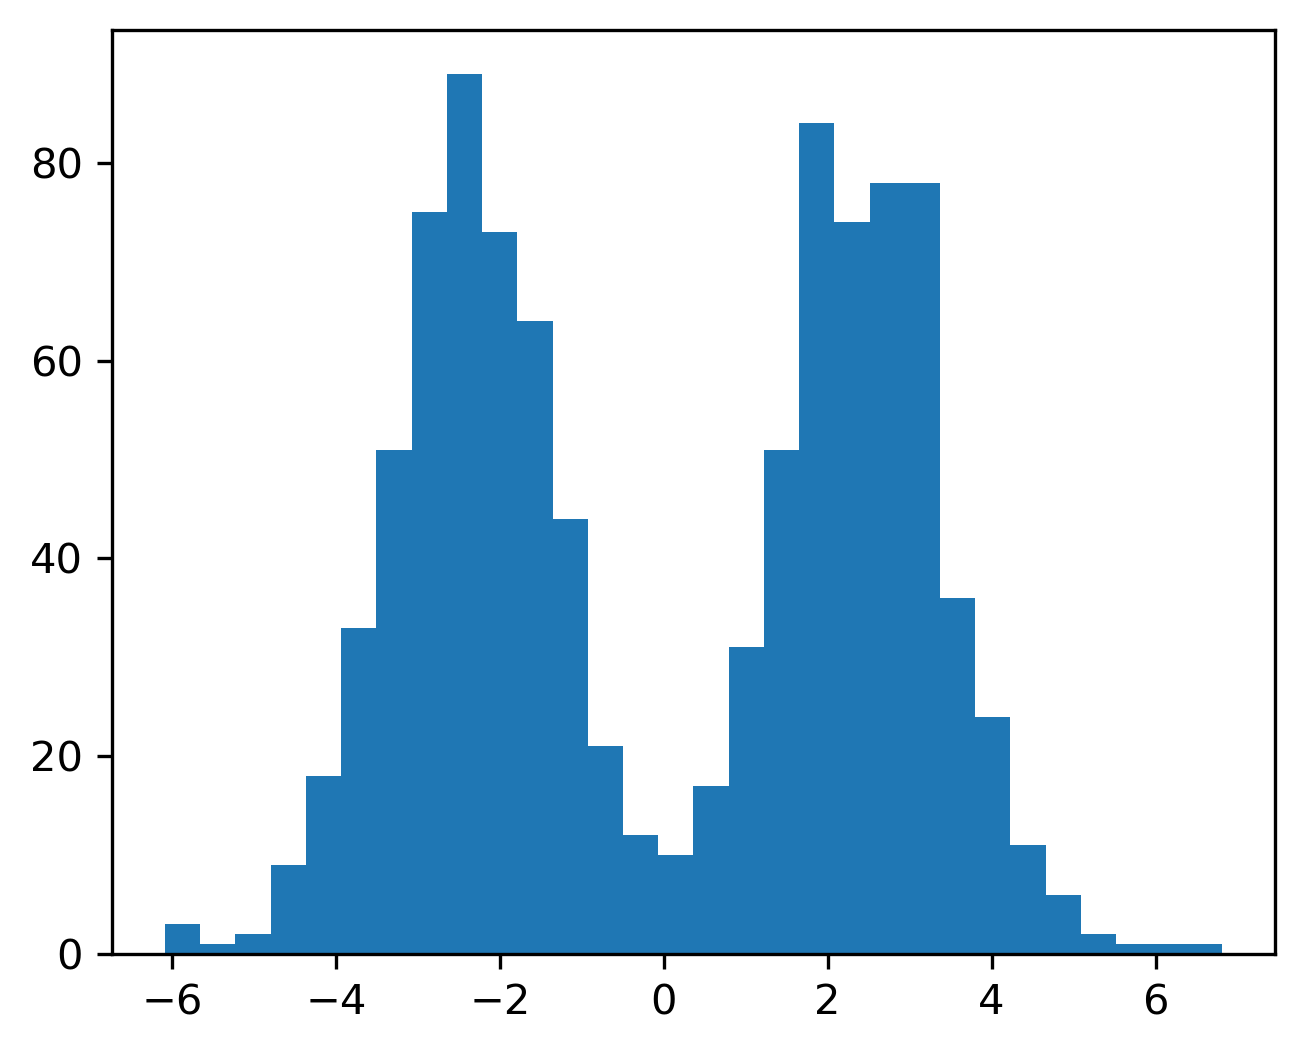
\includegraphics[width=0.48\linewidth]{images/2_cluster_hist_t_0.4.png}
                \caption{Распределение синтетического набора данных с параметром \(t = 0.4\).}
                \label{fig:synthetic:t:0.4}
            \end{figure}

            \begin{figure}[H]\centering
                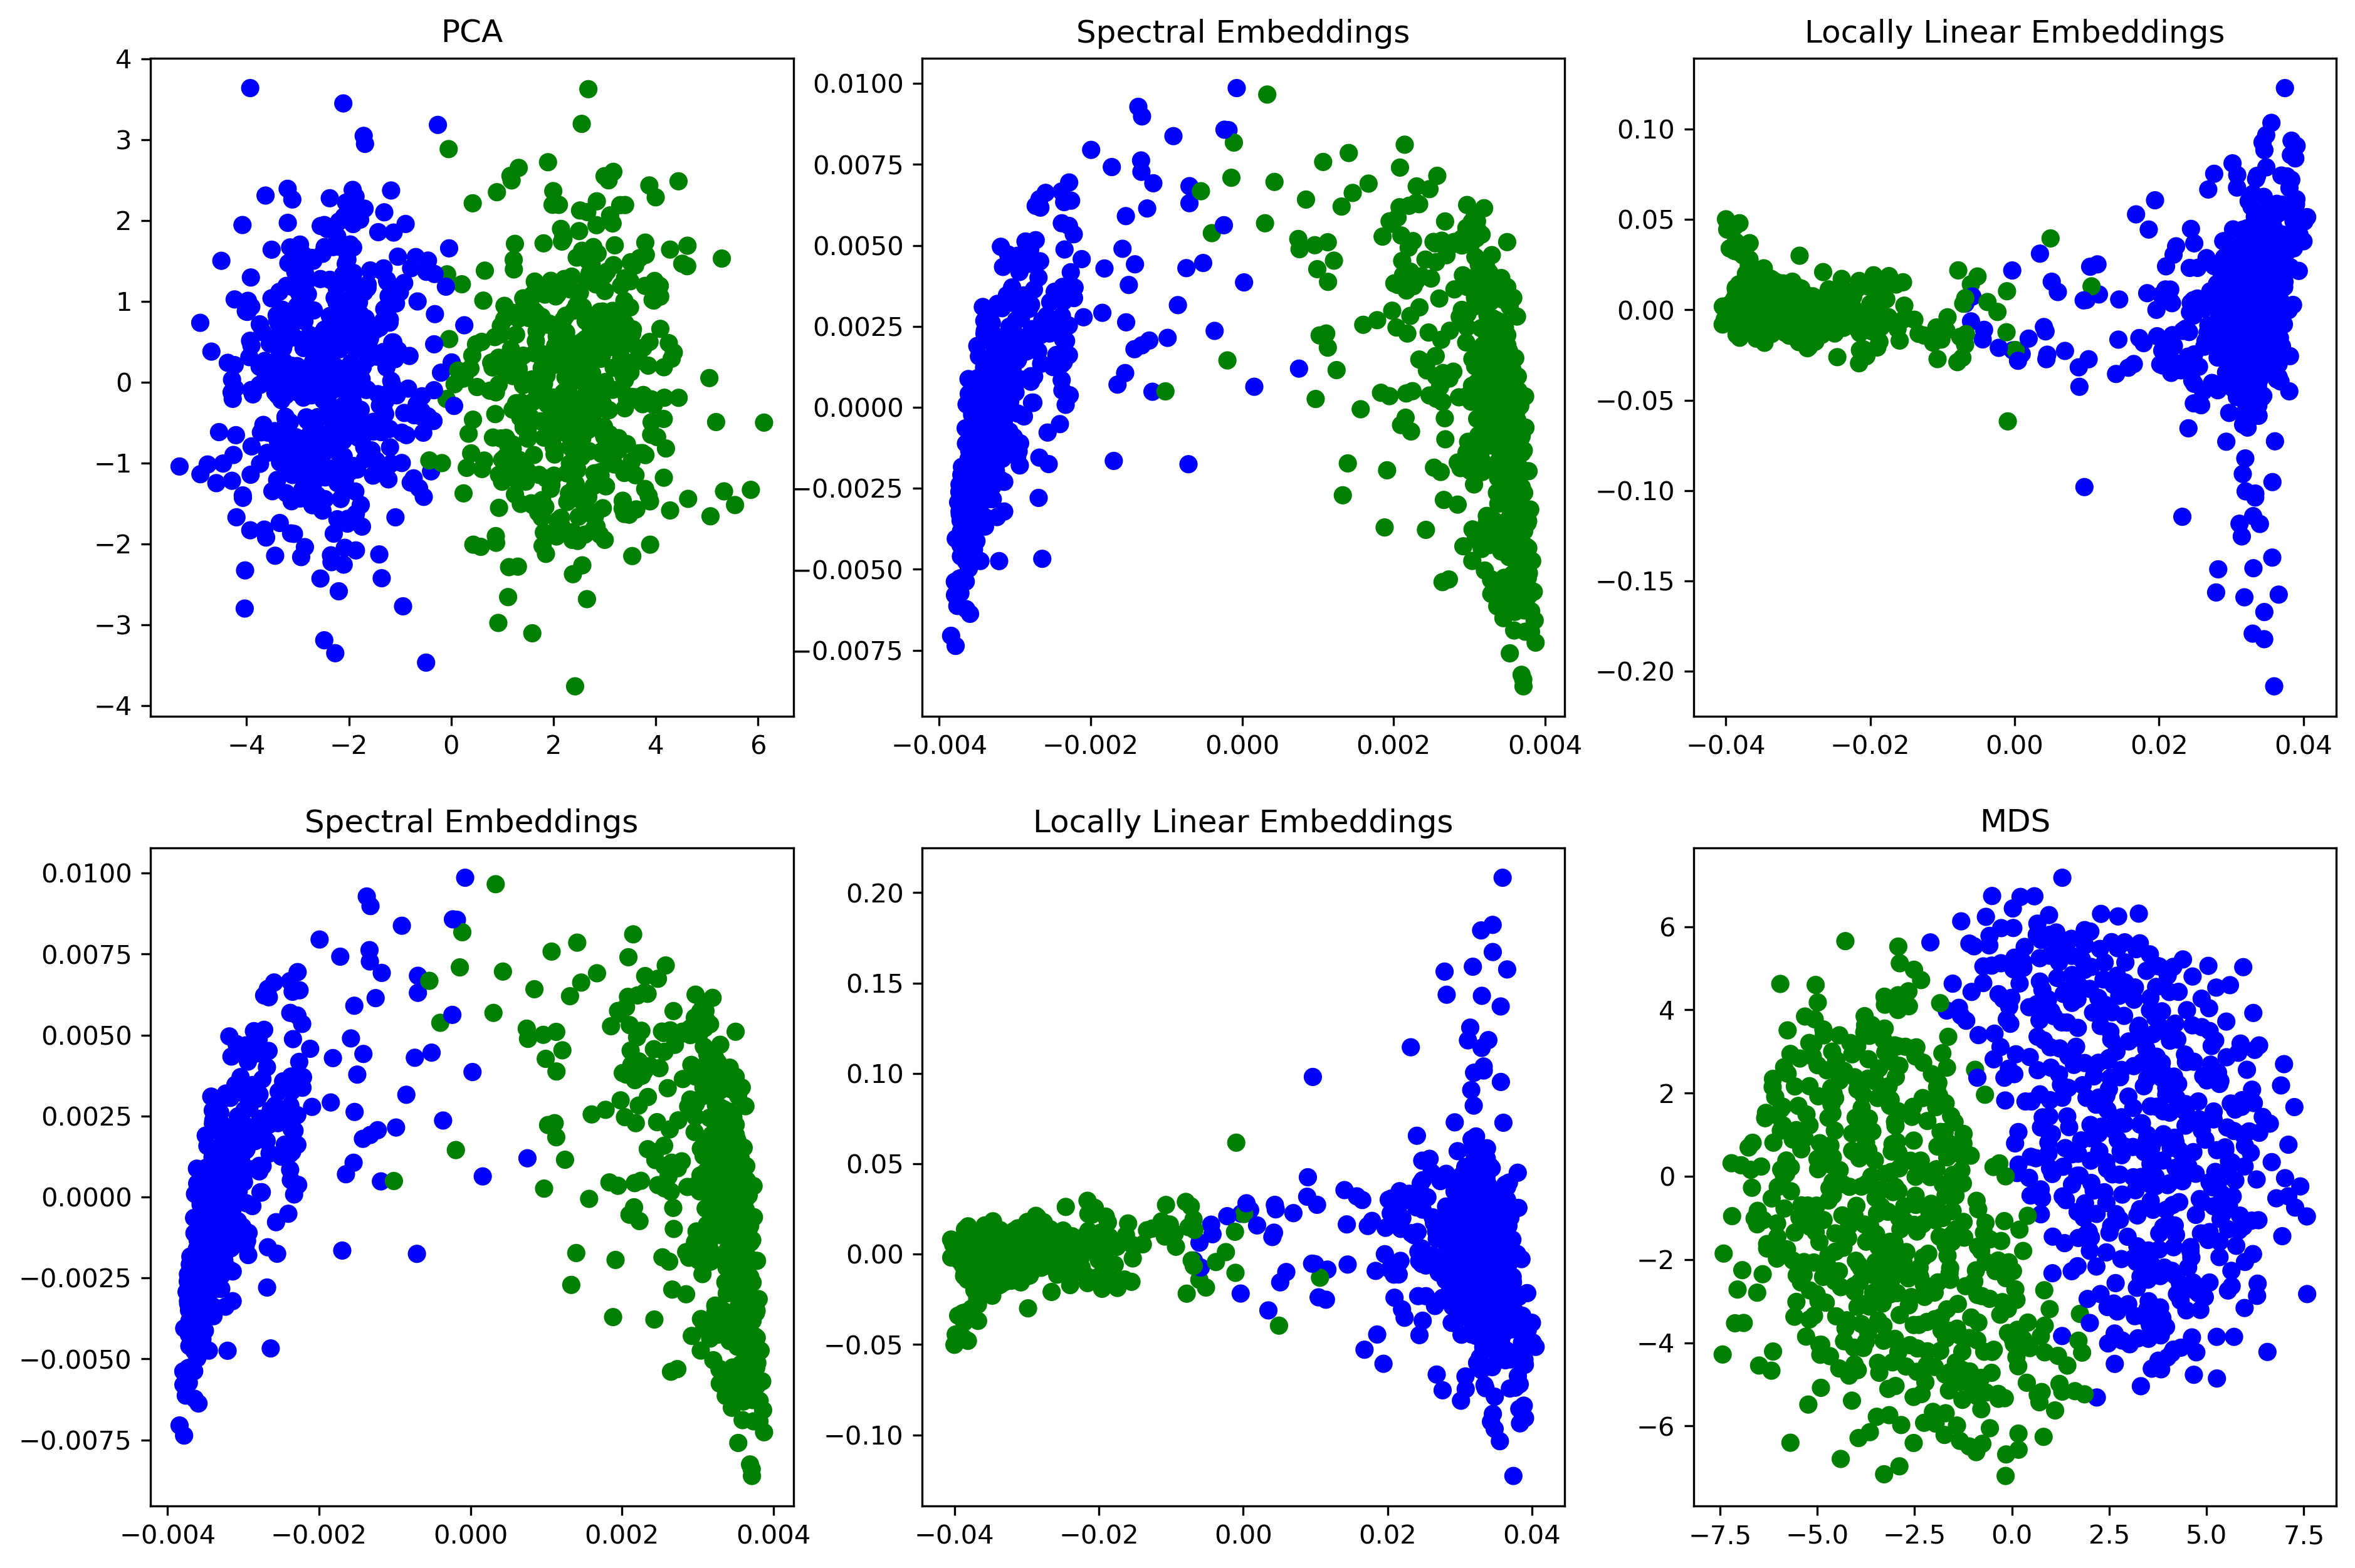
\includegraphics[width=0.99\linewidth]{images/decomposer/2_cluster_decomposer_analysis_t_0.4.png}
                \caption{Визуализация синтетических данных с параметром \(t = 0.4\) после снижения размерности с 20 до 2 с использованием PCA, Spectral Embeddings, Locally Linear Embeddings, MDS, ISOMAP, UMAP.}
                \label{fig:synthetic:t:0.4:example}
            \end{figure}

            Исходя из графиков, можно выделить явного лидера -- метод PCA, который стабильно показывает максимальные значения метрик (порядка 0.9 и выше) при любом количестве компонент. Это указывает на эффективное сохранение линейной структуры синтетических данных, особенно в случаях, когда кластеры умеренно разделены. MDS, а также ISOMAP и UMAP, дают сопоставимо высокие результаты, практически не зависящие от количества компонент, что говорит о слабой деградации качества даже при сильном снижении размерности данных. Locally Linear Embeddings и Spectral Embeddings, напротив, демонстрируют выраженную чувствительность к размерности. С уменьшением числа компонент качество кластеризации постепенно улучшается и достигает пика на размерности равной числу заложенных кластеров.

            \begin{figure}[H]\centering
                \subfigure[]{
                    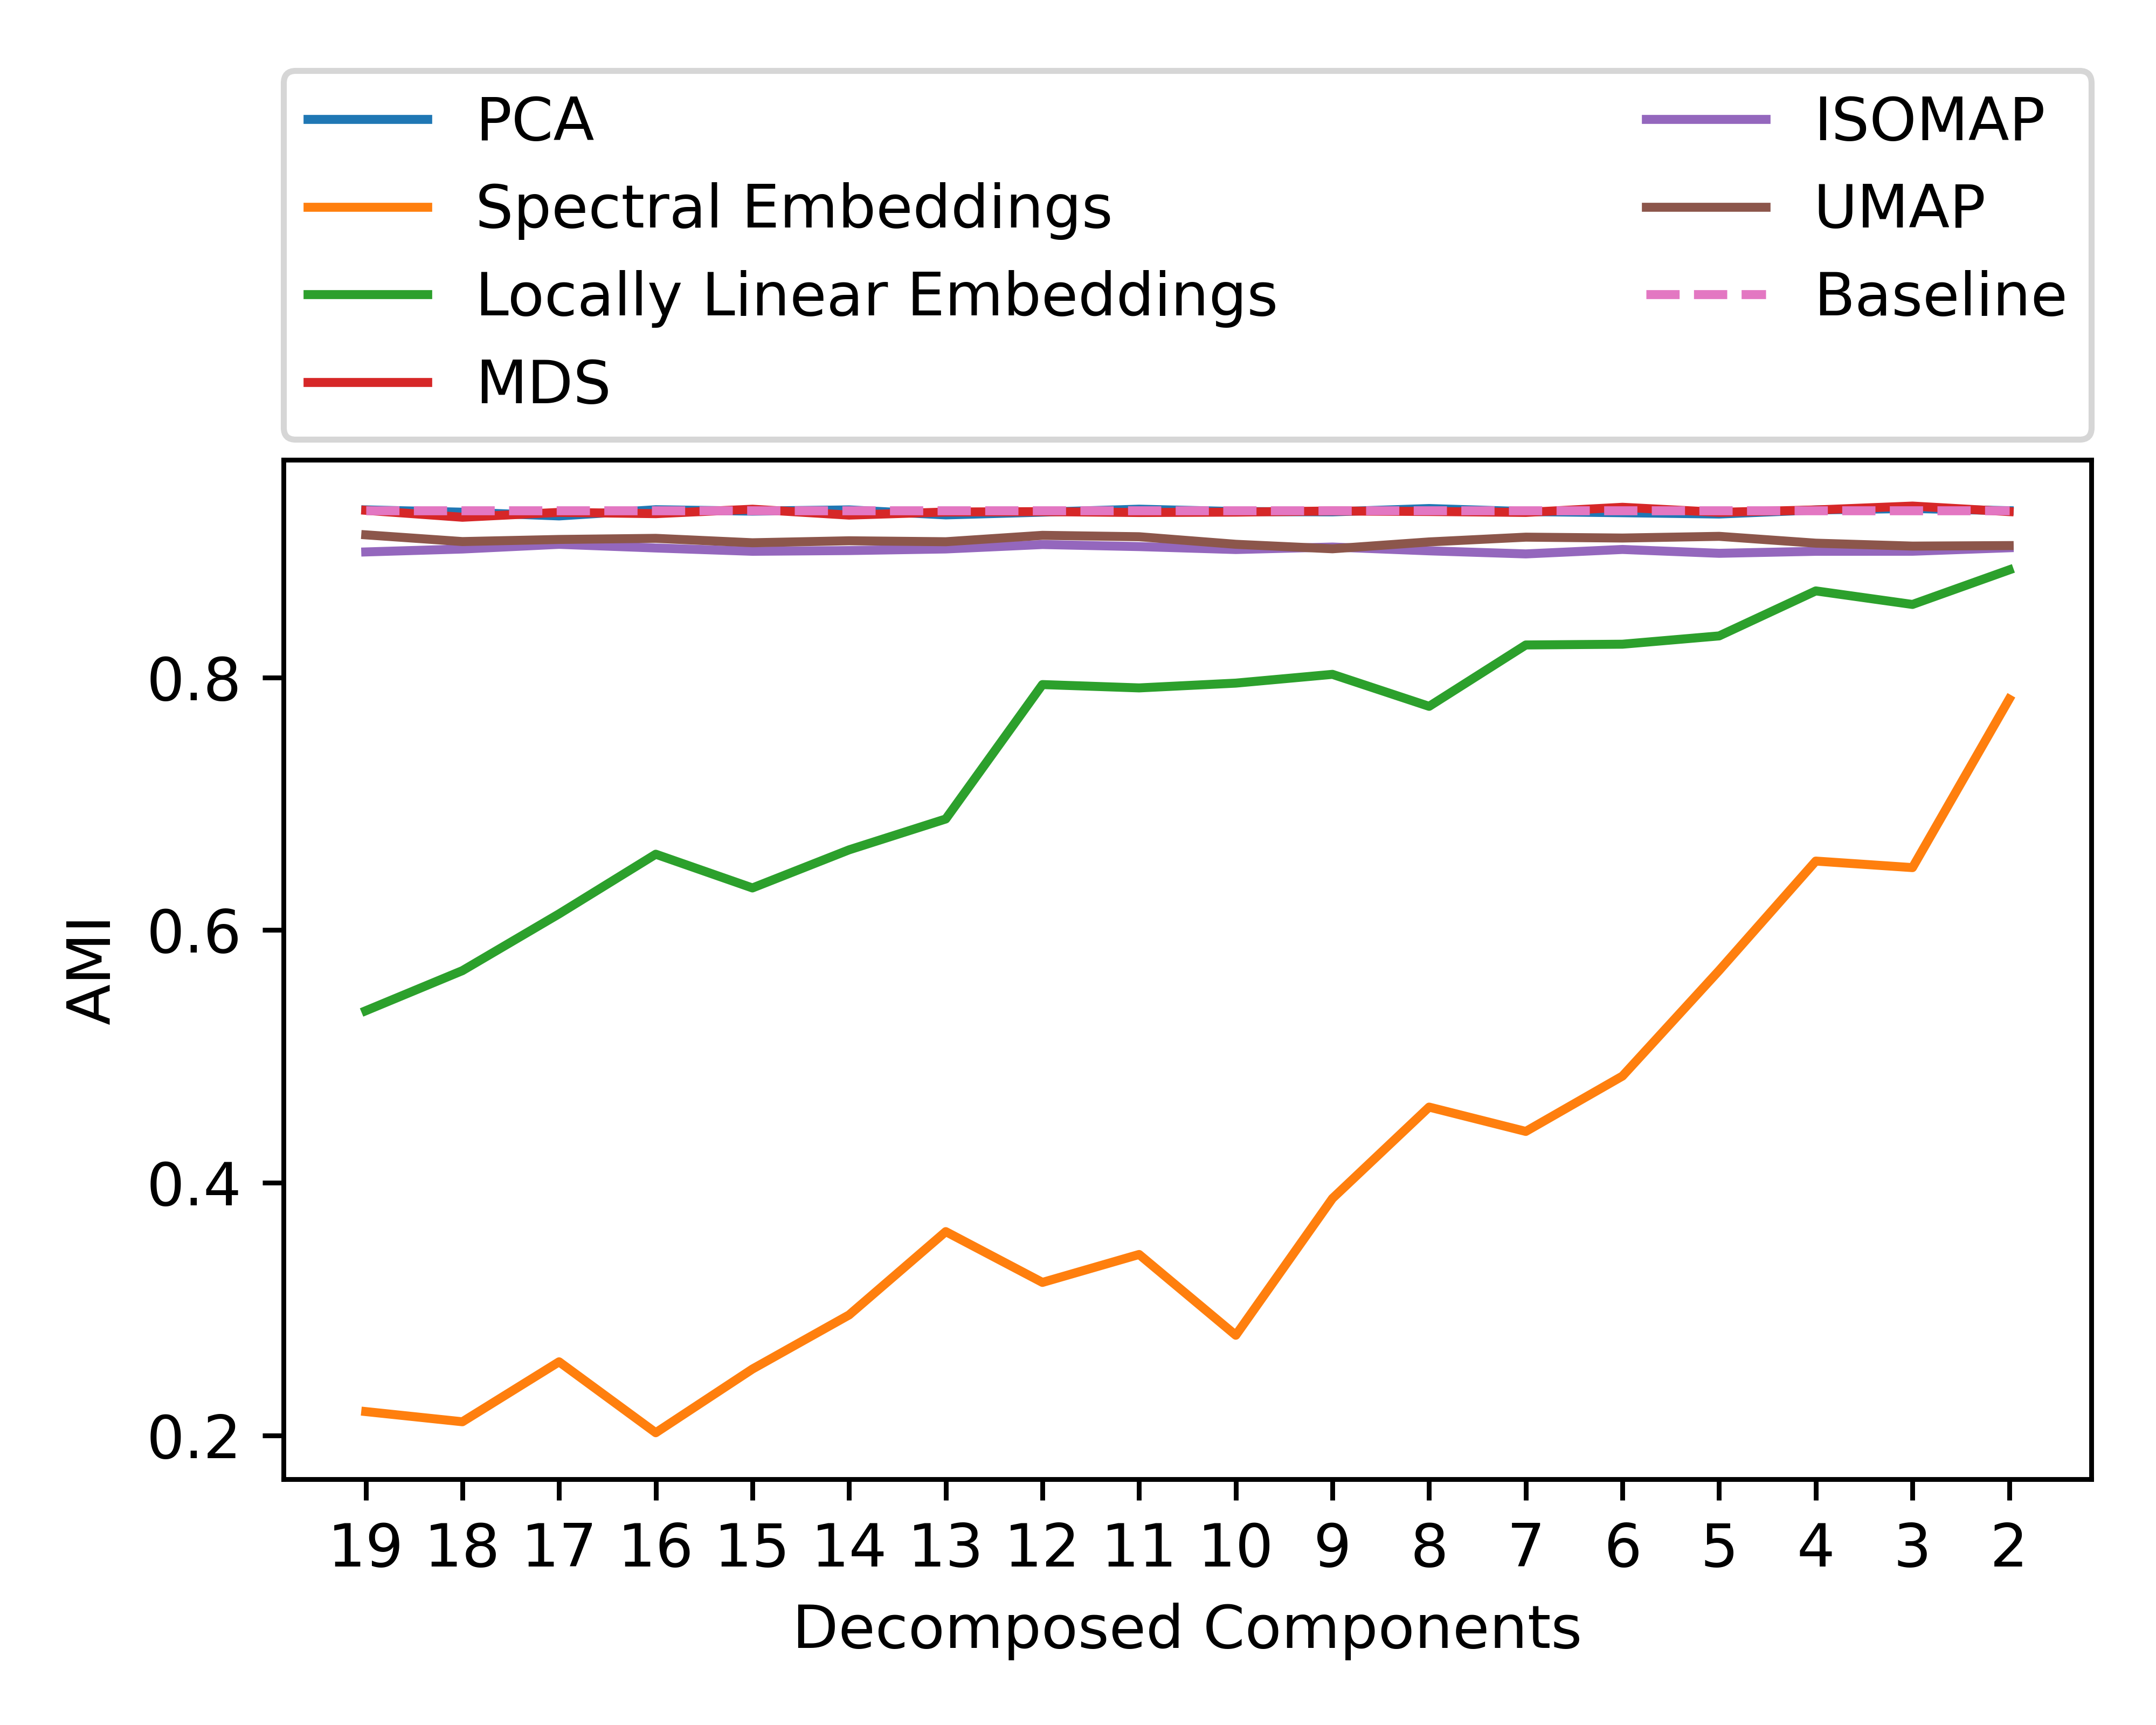
\includegraphics[width=0.48\linewidth]{images/charts/detailed_decomposition_metric_t_0.4_p_2_comparison_2_clusters_ami.png}
                    \label{subfig:synthetic:t_0.4:dim_influence:ami}
                }
                \subfigure[]{
                    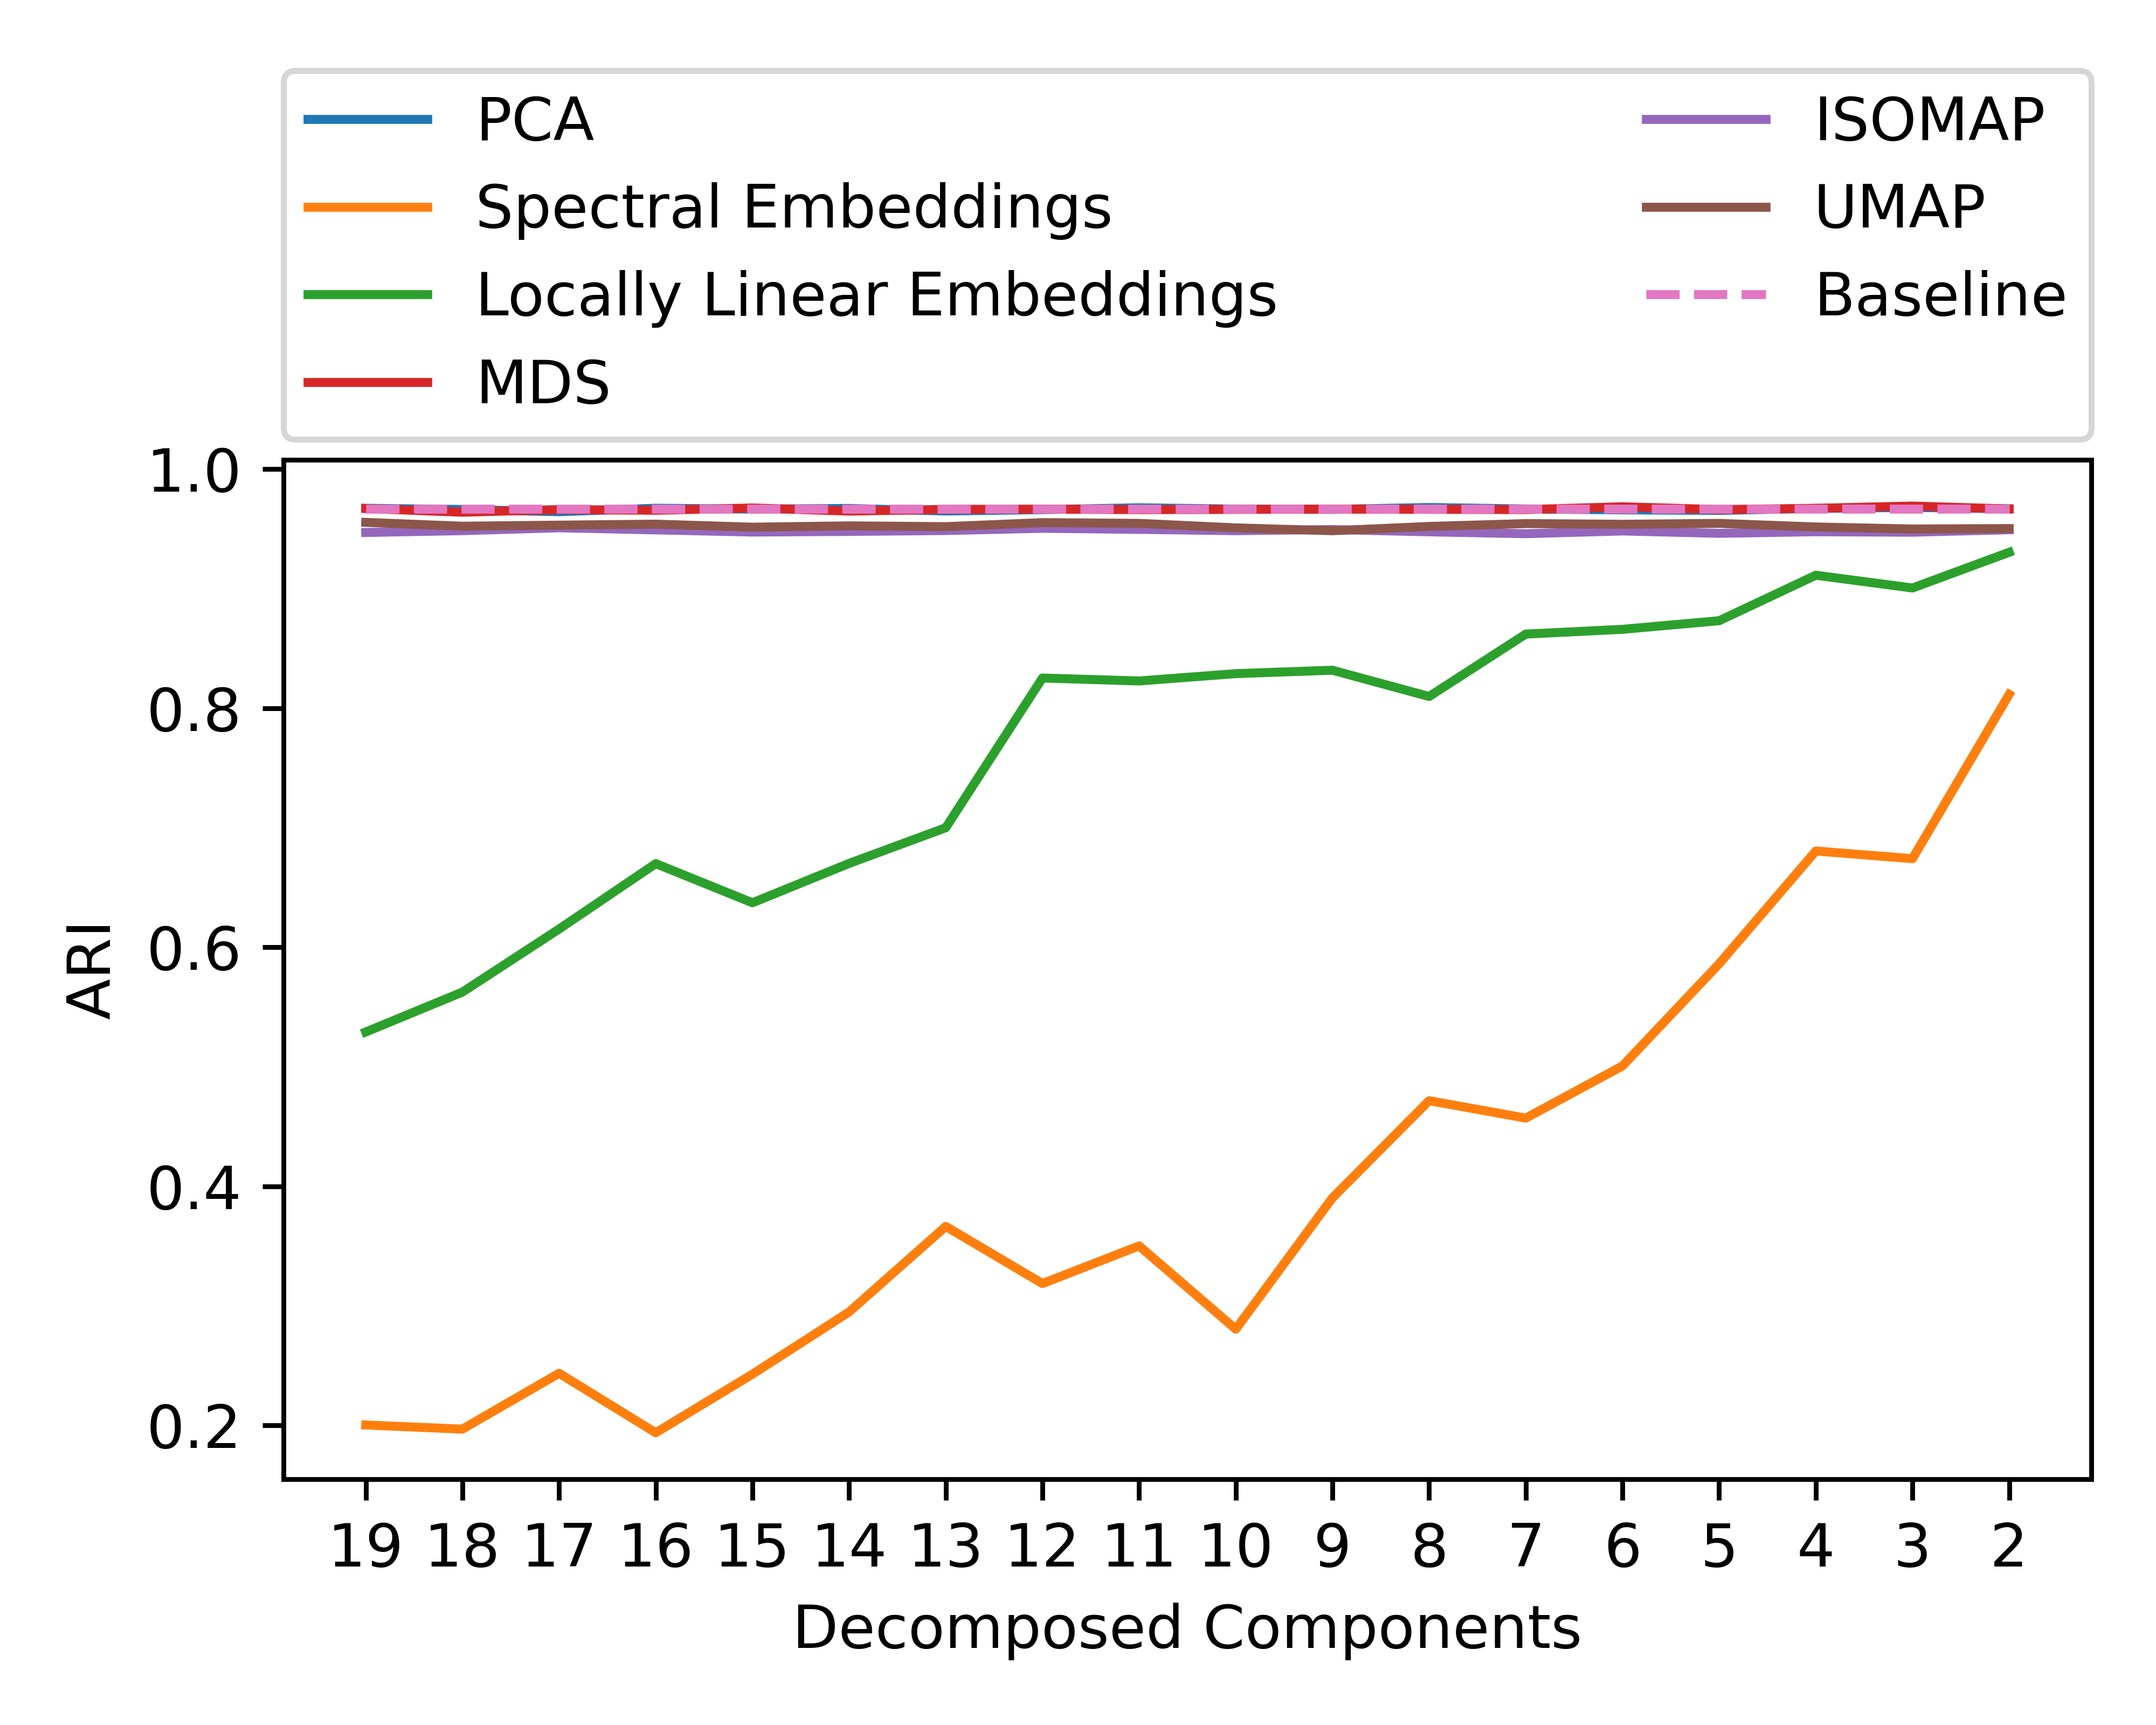
\includegraphics[width=0.48\linewidth]{images/charts/detailed_decomposition_metric_t_0.4_p_2_comparison_2_clusters_ari.png}
                    \label{subfig:synthetic:t_0.4:dim_influence:ari}
                }
                \subfigure[]{
                    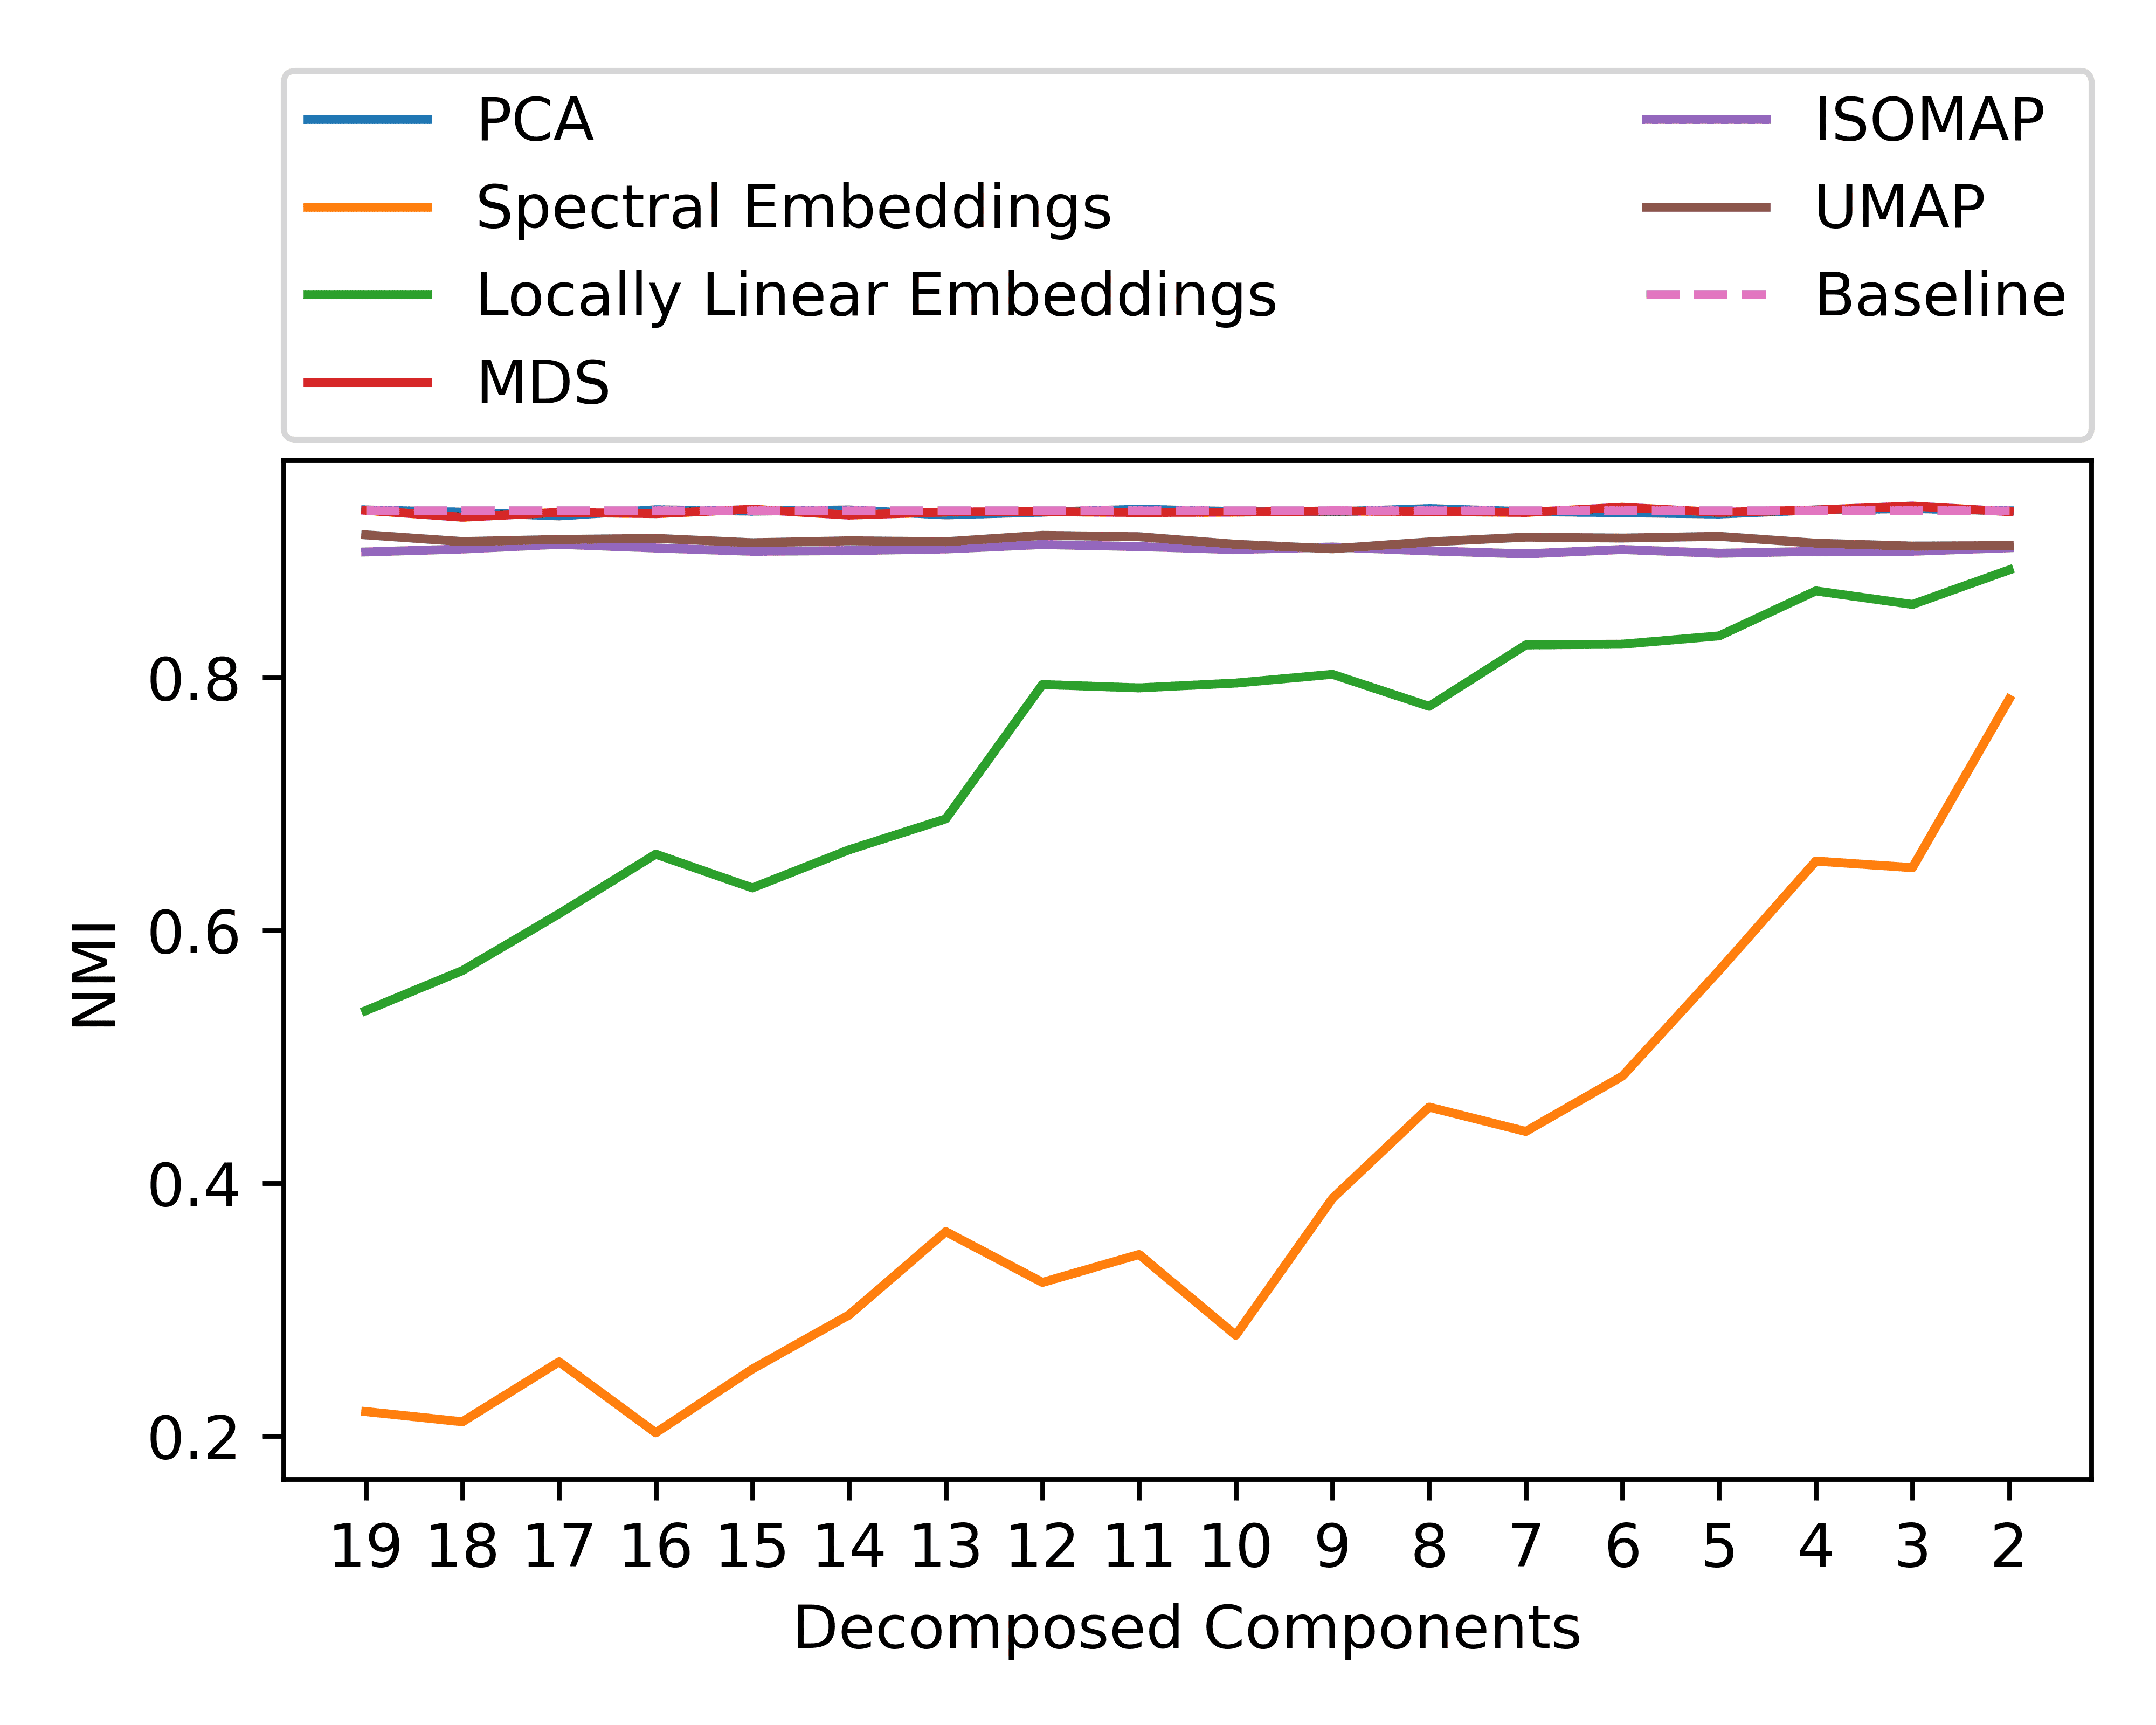
\includegraphics[width=0.48\linewidth]{images/charts/detailed_decomposition_metric_t_0.4_p_2_comparison_2_clusters_nmi.png}
                    \label{subfig:synthetic:t_0.4:dim_influence:nmi}
                }
                \subfigure[]{
                    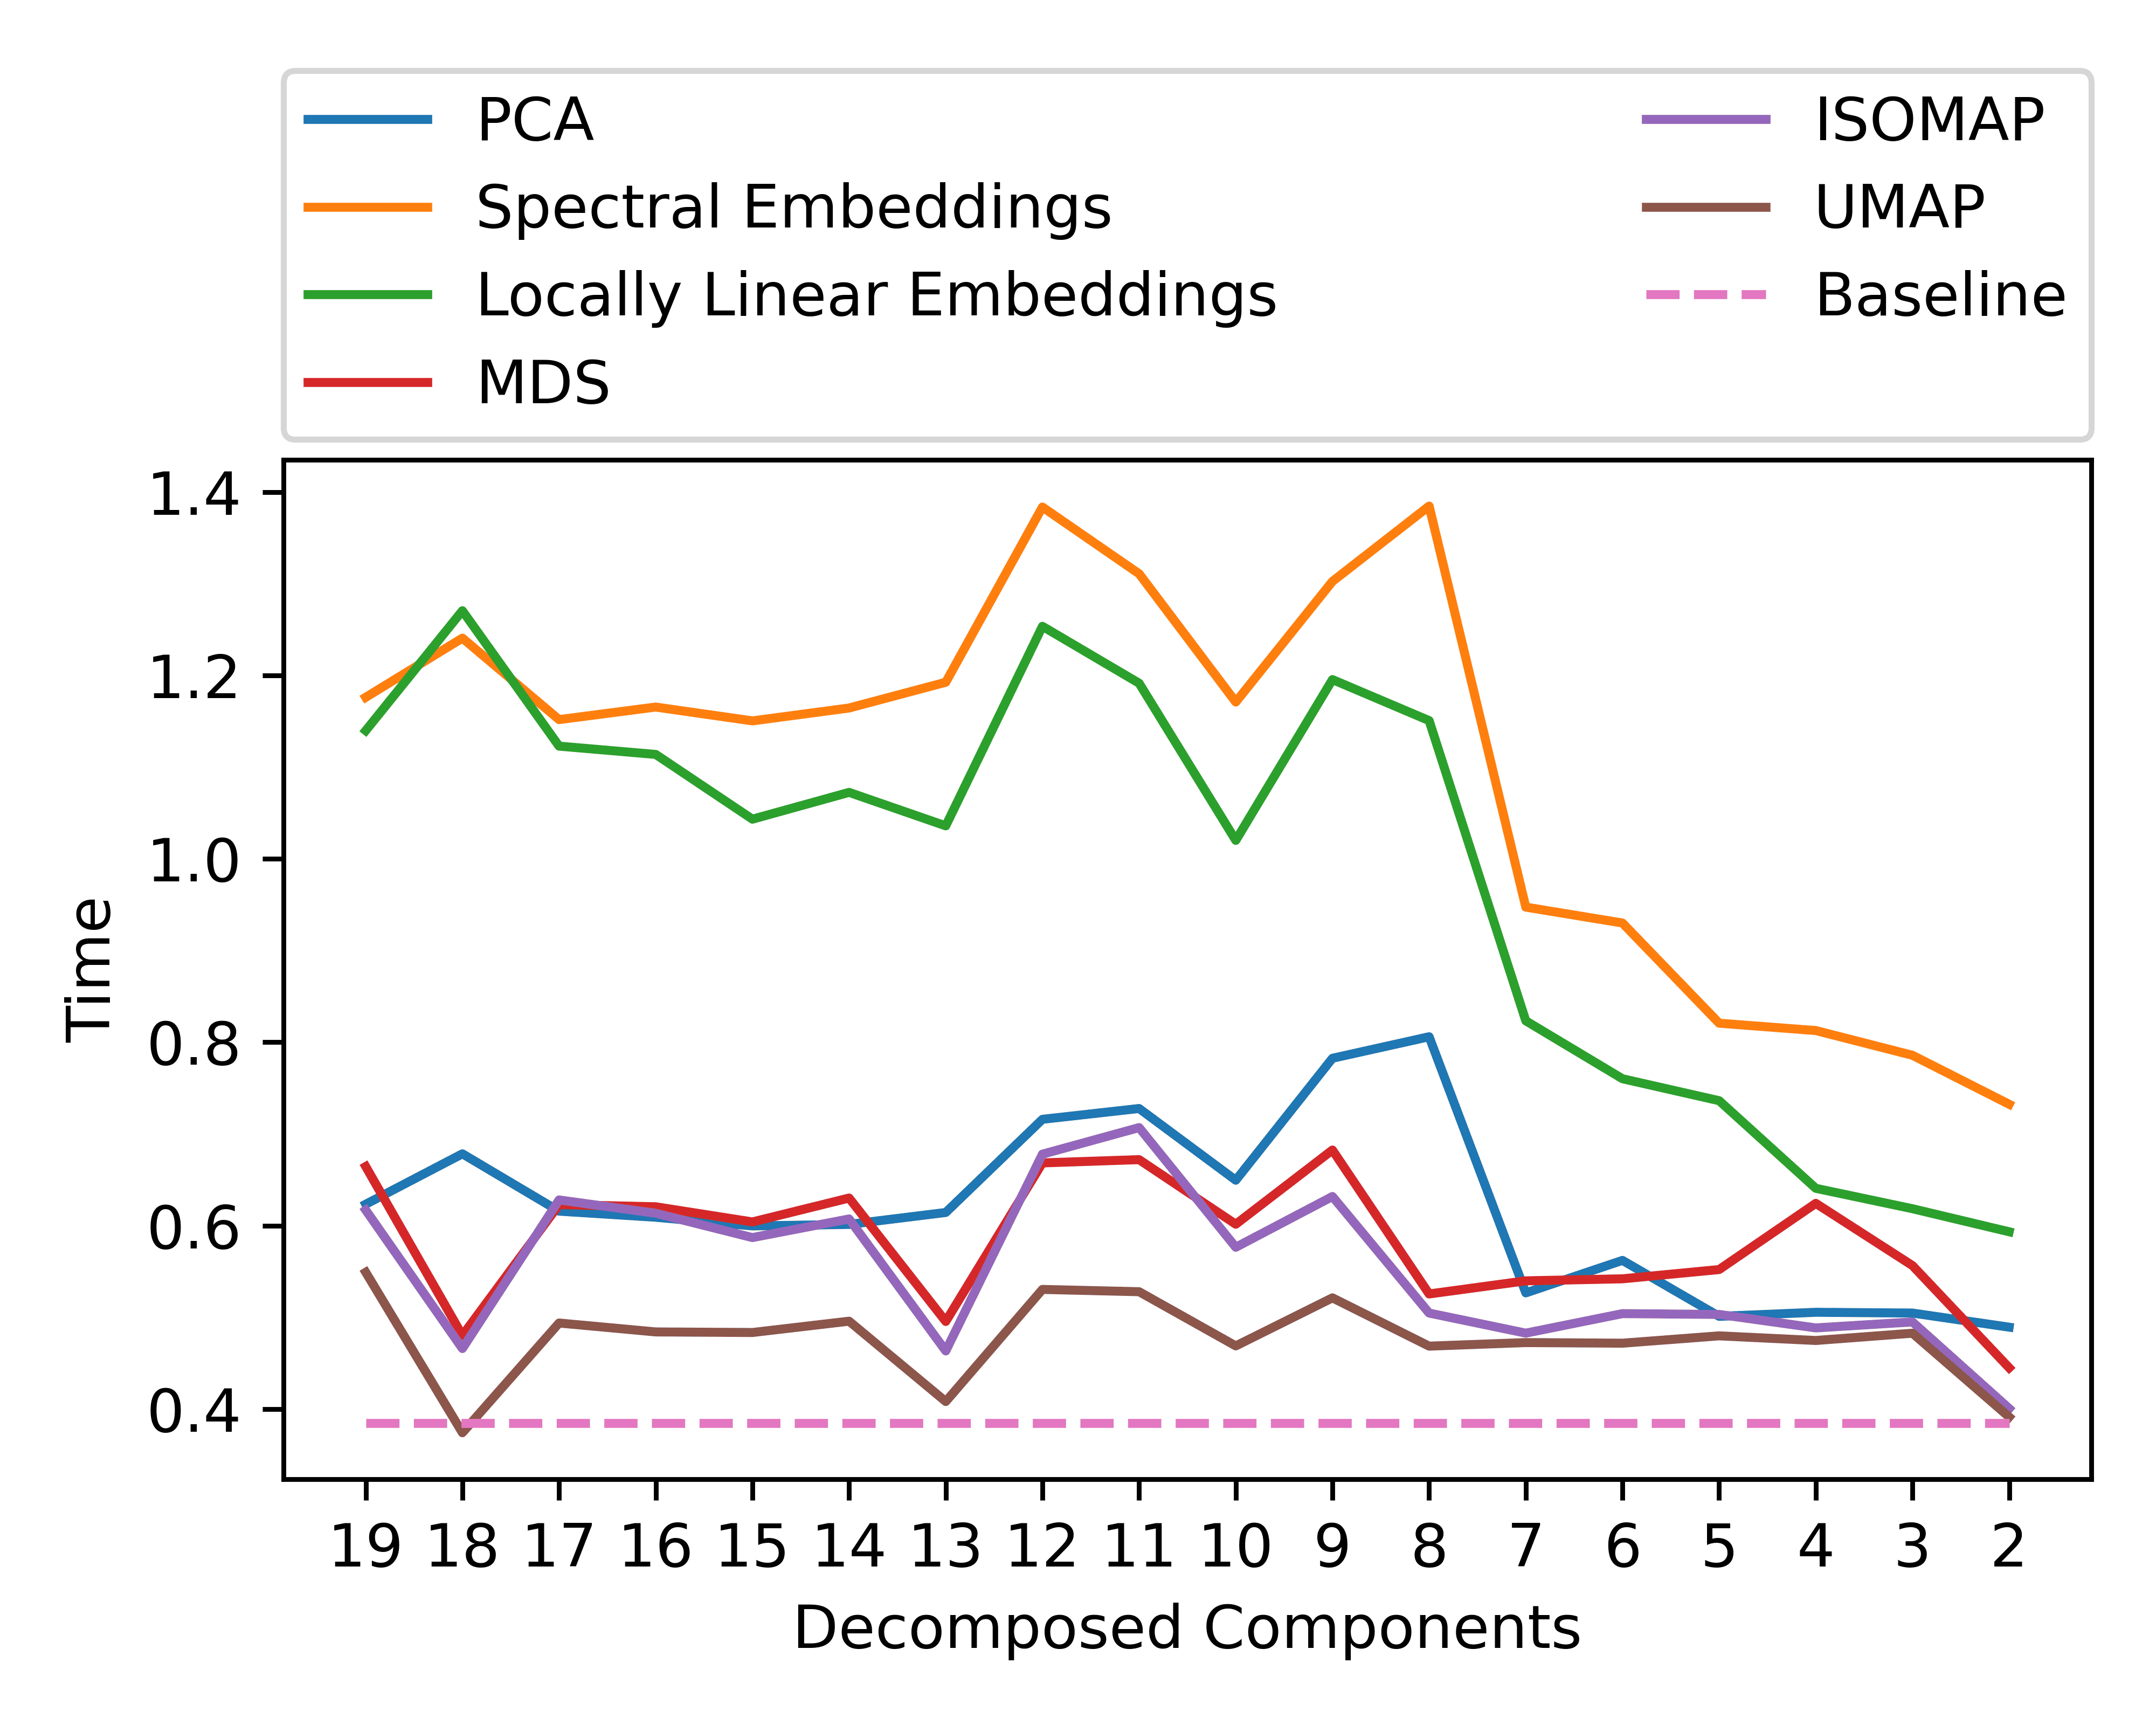
\includegraphics[width=0.48\linewidth]{images/charts/detailed_decomposition_metric_t_0.4_p_2_comparison_2_clusters_time.png}
                    \label{subfig:synthetic:t_0.4:dim_influence:time}
                }
                \caption{Анализ влияния размерности данных при различных методах снижения размерности на кластеризацию синтетического набора данных с параметром \(t = 0.4\). Линия Baseline -- результат работы алгоритма \kmeans{} без предварительного снижения размерности. Результаты для
                    \subref{subfig:synthetic:t_0.4:dim_influence:ami} AMI;
                    \subref{subfig:synthetic:t_0.4:dim_influence:ari} ARI;
                    \subref{subfig:synthetic:t_0.4:dim_influence:nmi} NMI, а также на время работы алгоритма \subref{subfig:synthetic:t_influence:time}.
                }
                \label{fig:synthetic:t_0.4:dim_influence}
            \end{figure}

            На рисунке \ref{fig:synthetic:t_0.8:dim_influence} представлен анализ влияния количества компонент, оставляемых после снижения размерности, на качество кластеризации при фиксированном значении параметра \(t = 0.8\), соответствующем сильному перекрытию кластеров (Рисунок \ref{fig:synthetic:t:0.8}). На этом уровне разделимость между группами минимальна, что делает задачу особенно чувствительной к качеству понижения размерности. Также, следует, что методы PCA демонстрирует наилучшую устойчивость и качество кластеризации вне зависимости от числа компонент. В противоположность, методы Locally Linear Embeddings и Spectral Embeddings показывают низкие и слабо возрастающие значения всех метрик при уменьшении количества компонент, что говорит о неэффективном представлении кластерной структуры в условиях высокой плотности и перекрытия. Рисунок \ref{fig:synthetic:t:0.8:example} отображает распределение точек в пространстве меньшей размерности после применения методов снижения размерности PCA, Spectral Embeddings, Locally Linear Embeddings, MDS, ISOMAP, UMAP.

            \begin{figure}[H]\centering
                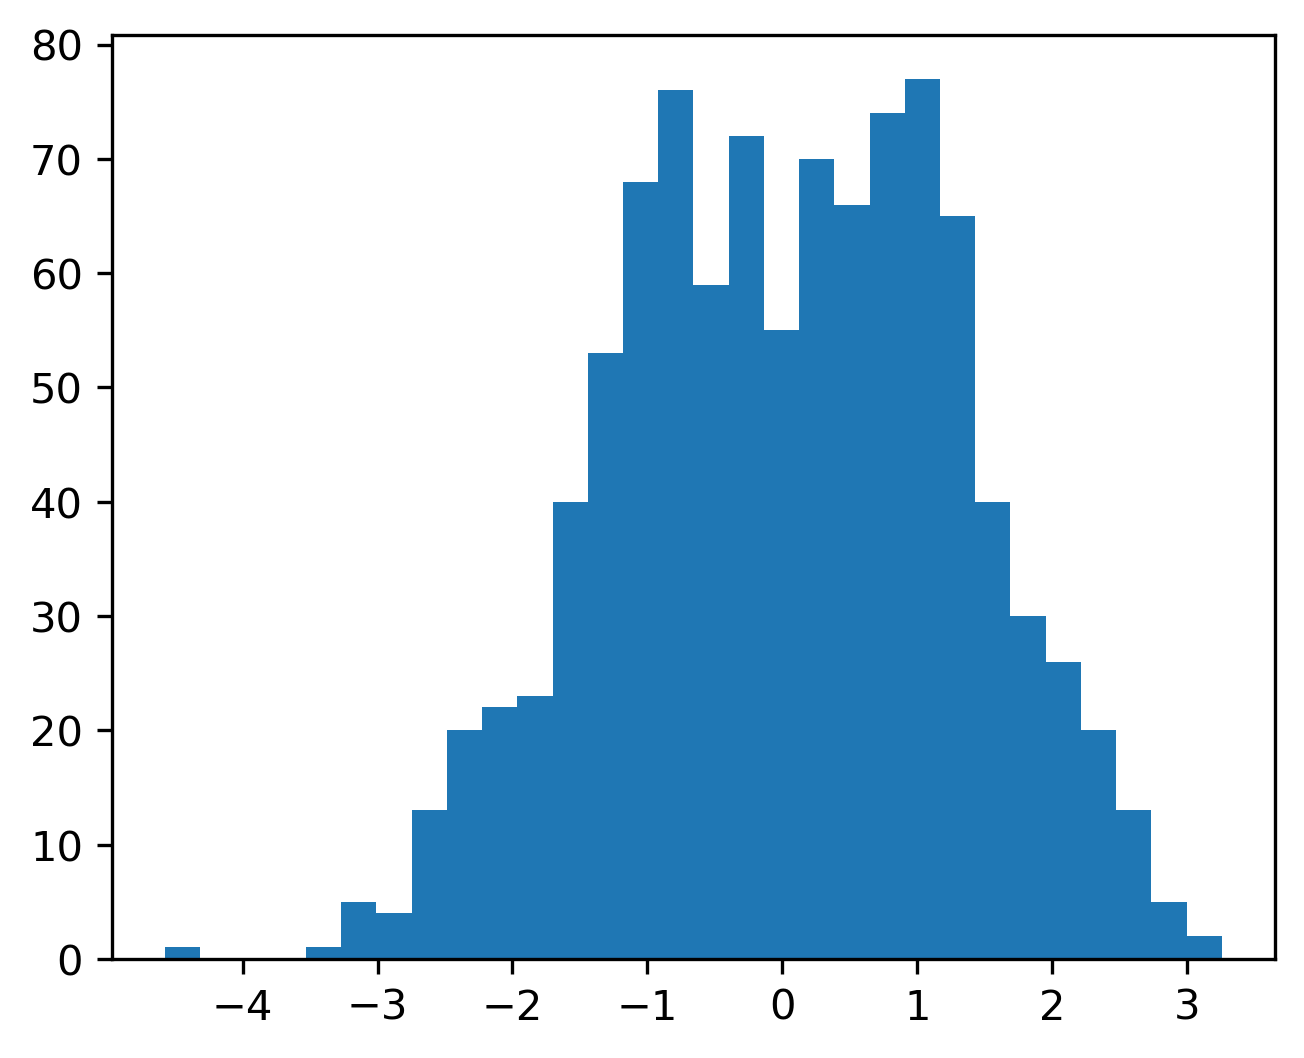
\includegraphics[width=0.48\linewidth]{images/2_cluster_hist_t_0.8.png}
                \caption{Распределение синтетического набора данных с параметром \(t = 0.8\).}
                \label{fig:synthetic:t:0.8}
            \end{figure}

            \begin{figure}[H]\centering
                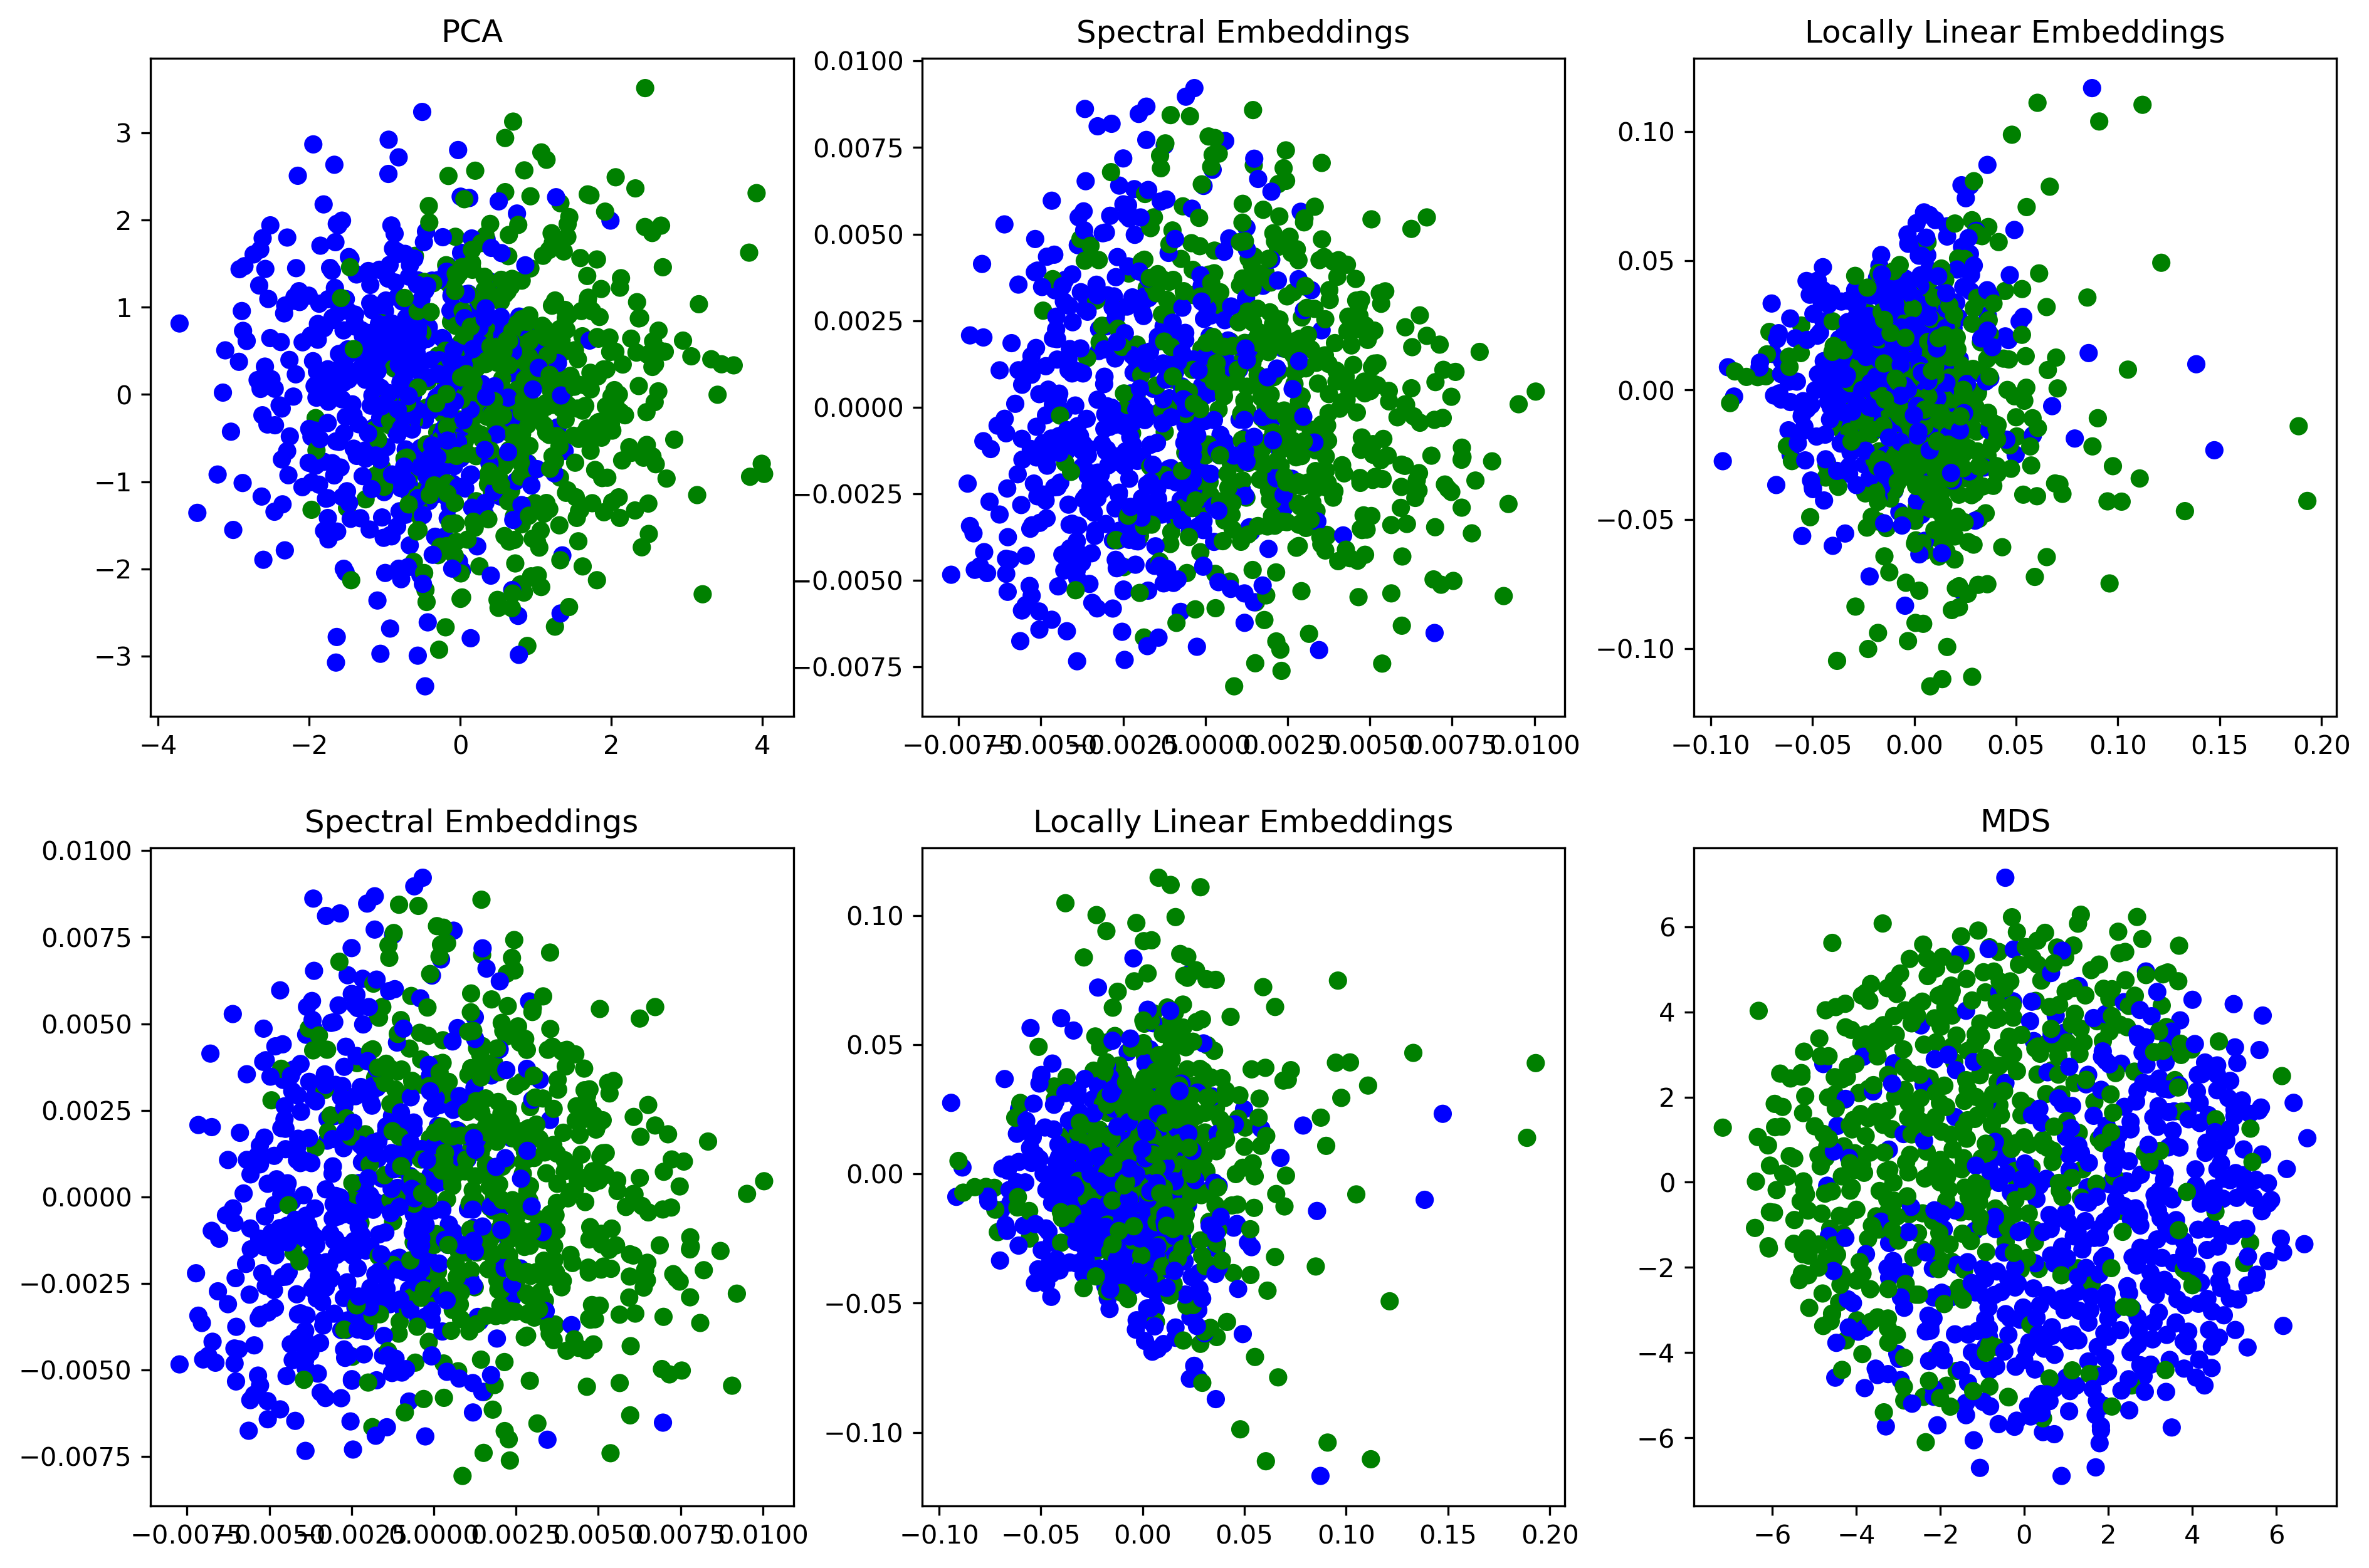
\includegraphics[width=0.99\linewidth]{images/decomposer/2_cluster_decomposer_analysis_t_0.8.png}
                \caption{Визуализация синтетических данных с параметром \(t = 0.8\) после снижения размерности с 20 до 2 с использованием PCA, Spectral Embeddings, Locally Linear Embeddings, MDS, ISOMAP, UMAP.}
                \label{fig:synthetic:t:0.8:example}
            \end{figure}

            Таким образом, при высоком уровне наложения кластеров (большое t) и варьируемом числе компонент, наиболее стабильные и надежные результаты обеспечивают методы PCA и MDS. Остальные методы, особенно LLE и Spectral, оказываются крайне чувствительными к размерности и не рекомендованы к применению в таких условиях.

            \begin{figure}[H]\centering
                \subfigure[]{
                    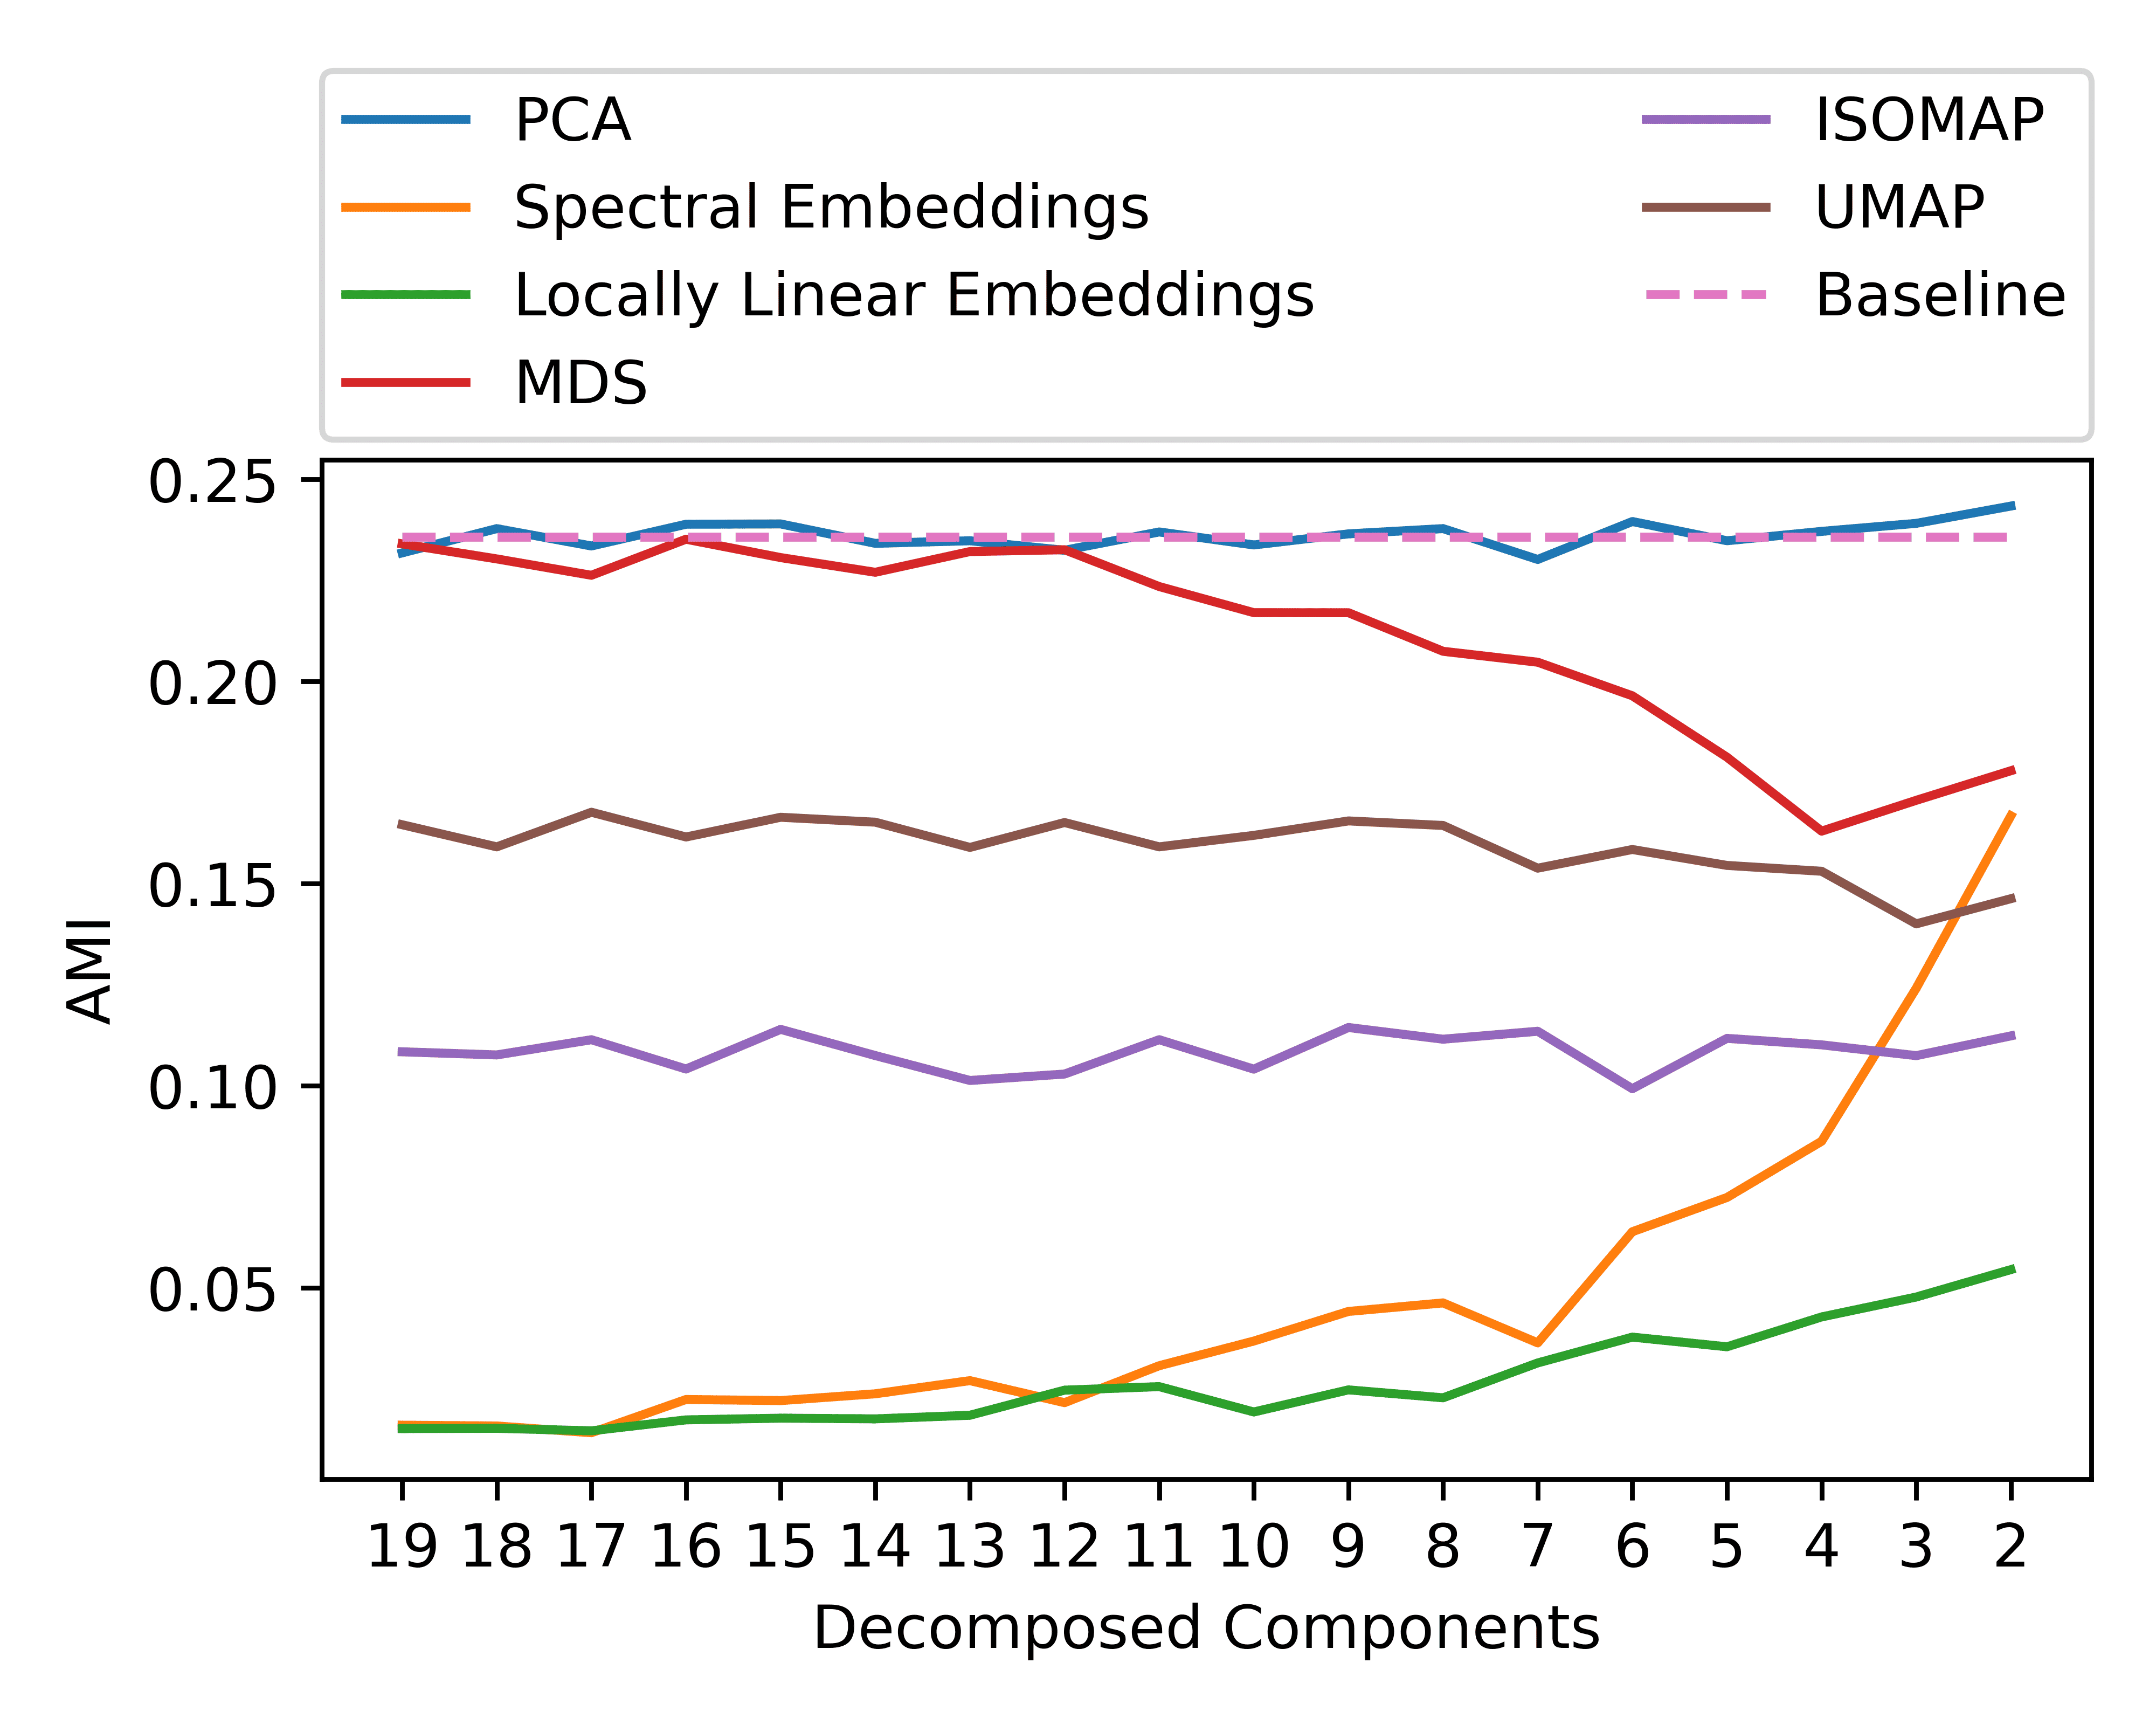
\includegraphics[width=0.48\linewidth]{images/charts/detailed_decomposition_metric_t_0.8_p_2_comparison_2_clusters_ami.png}
                    \label{subfig:synthetic:t_0.8:dim_influence:ami}
                }
                \subfigure[]{
                    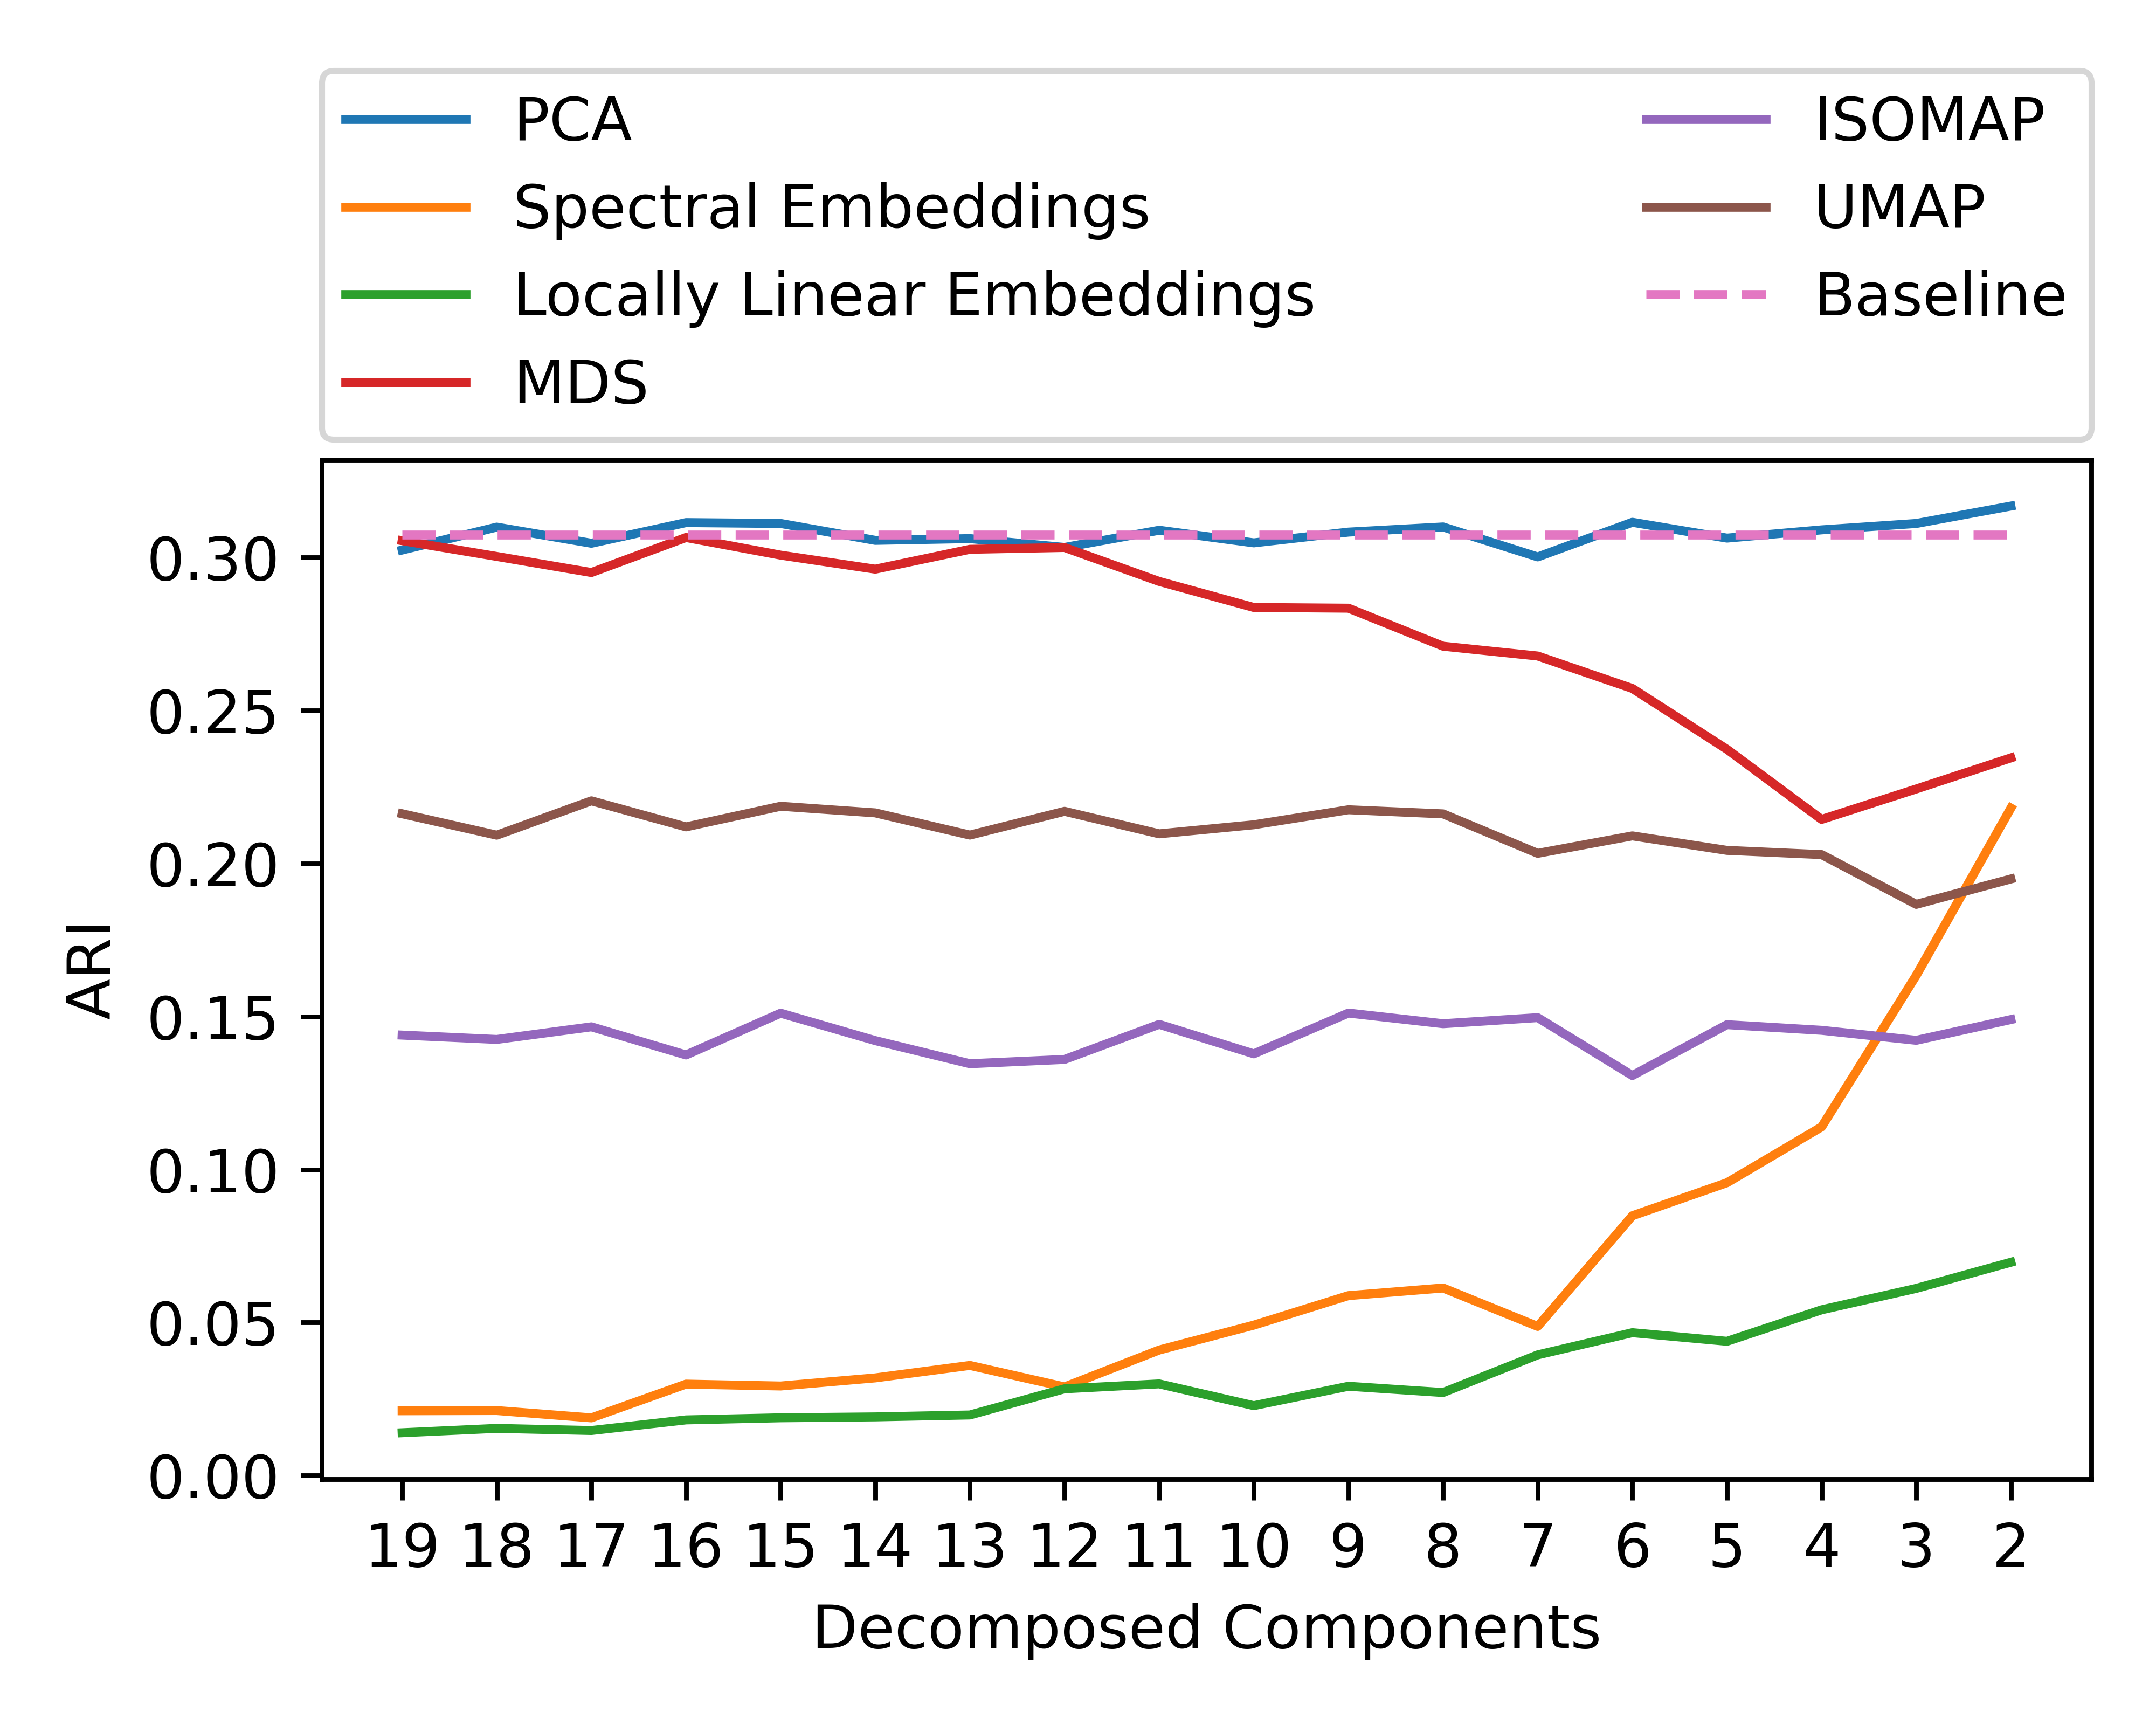
\includegraphics[width=0.48\linewidth]{images/charts/detailed_decomposition_metric_t_0.8_p_2_comparison_2_clusters_ari.png}
                    \label{subfig:synthetic:t_0.8:dim_influence:ari}
                }
                \subfigure[]{
                    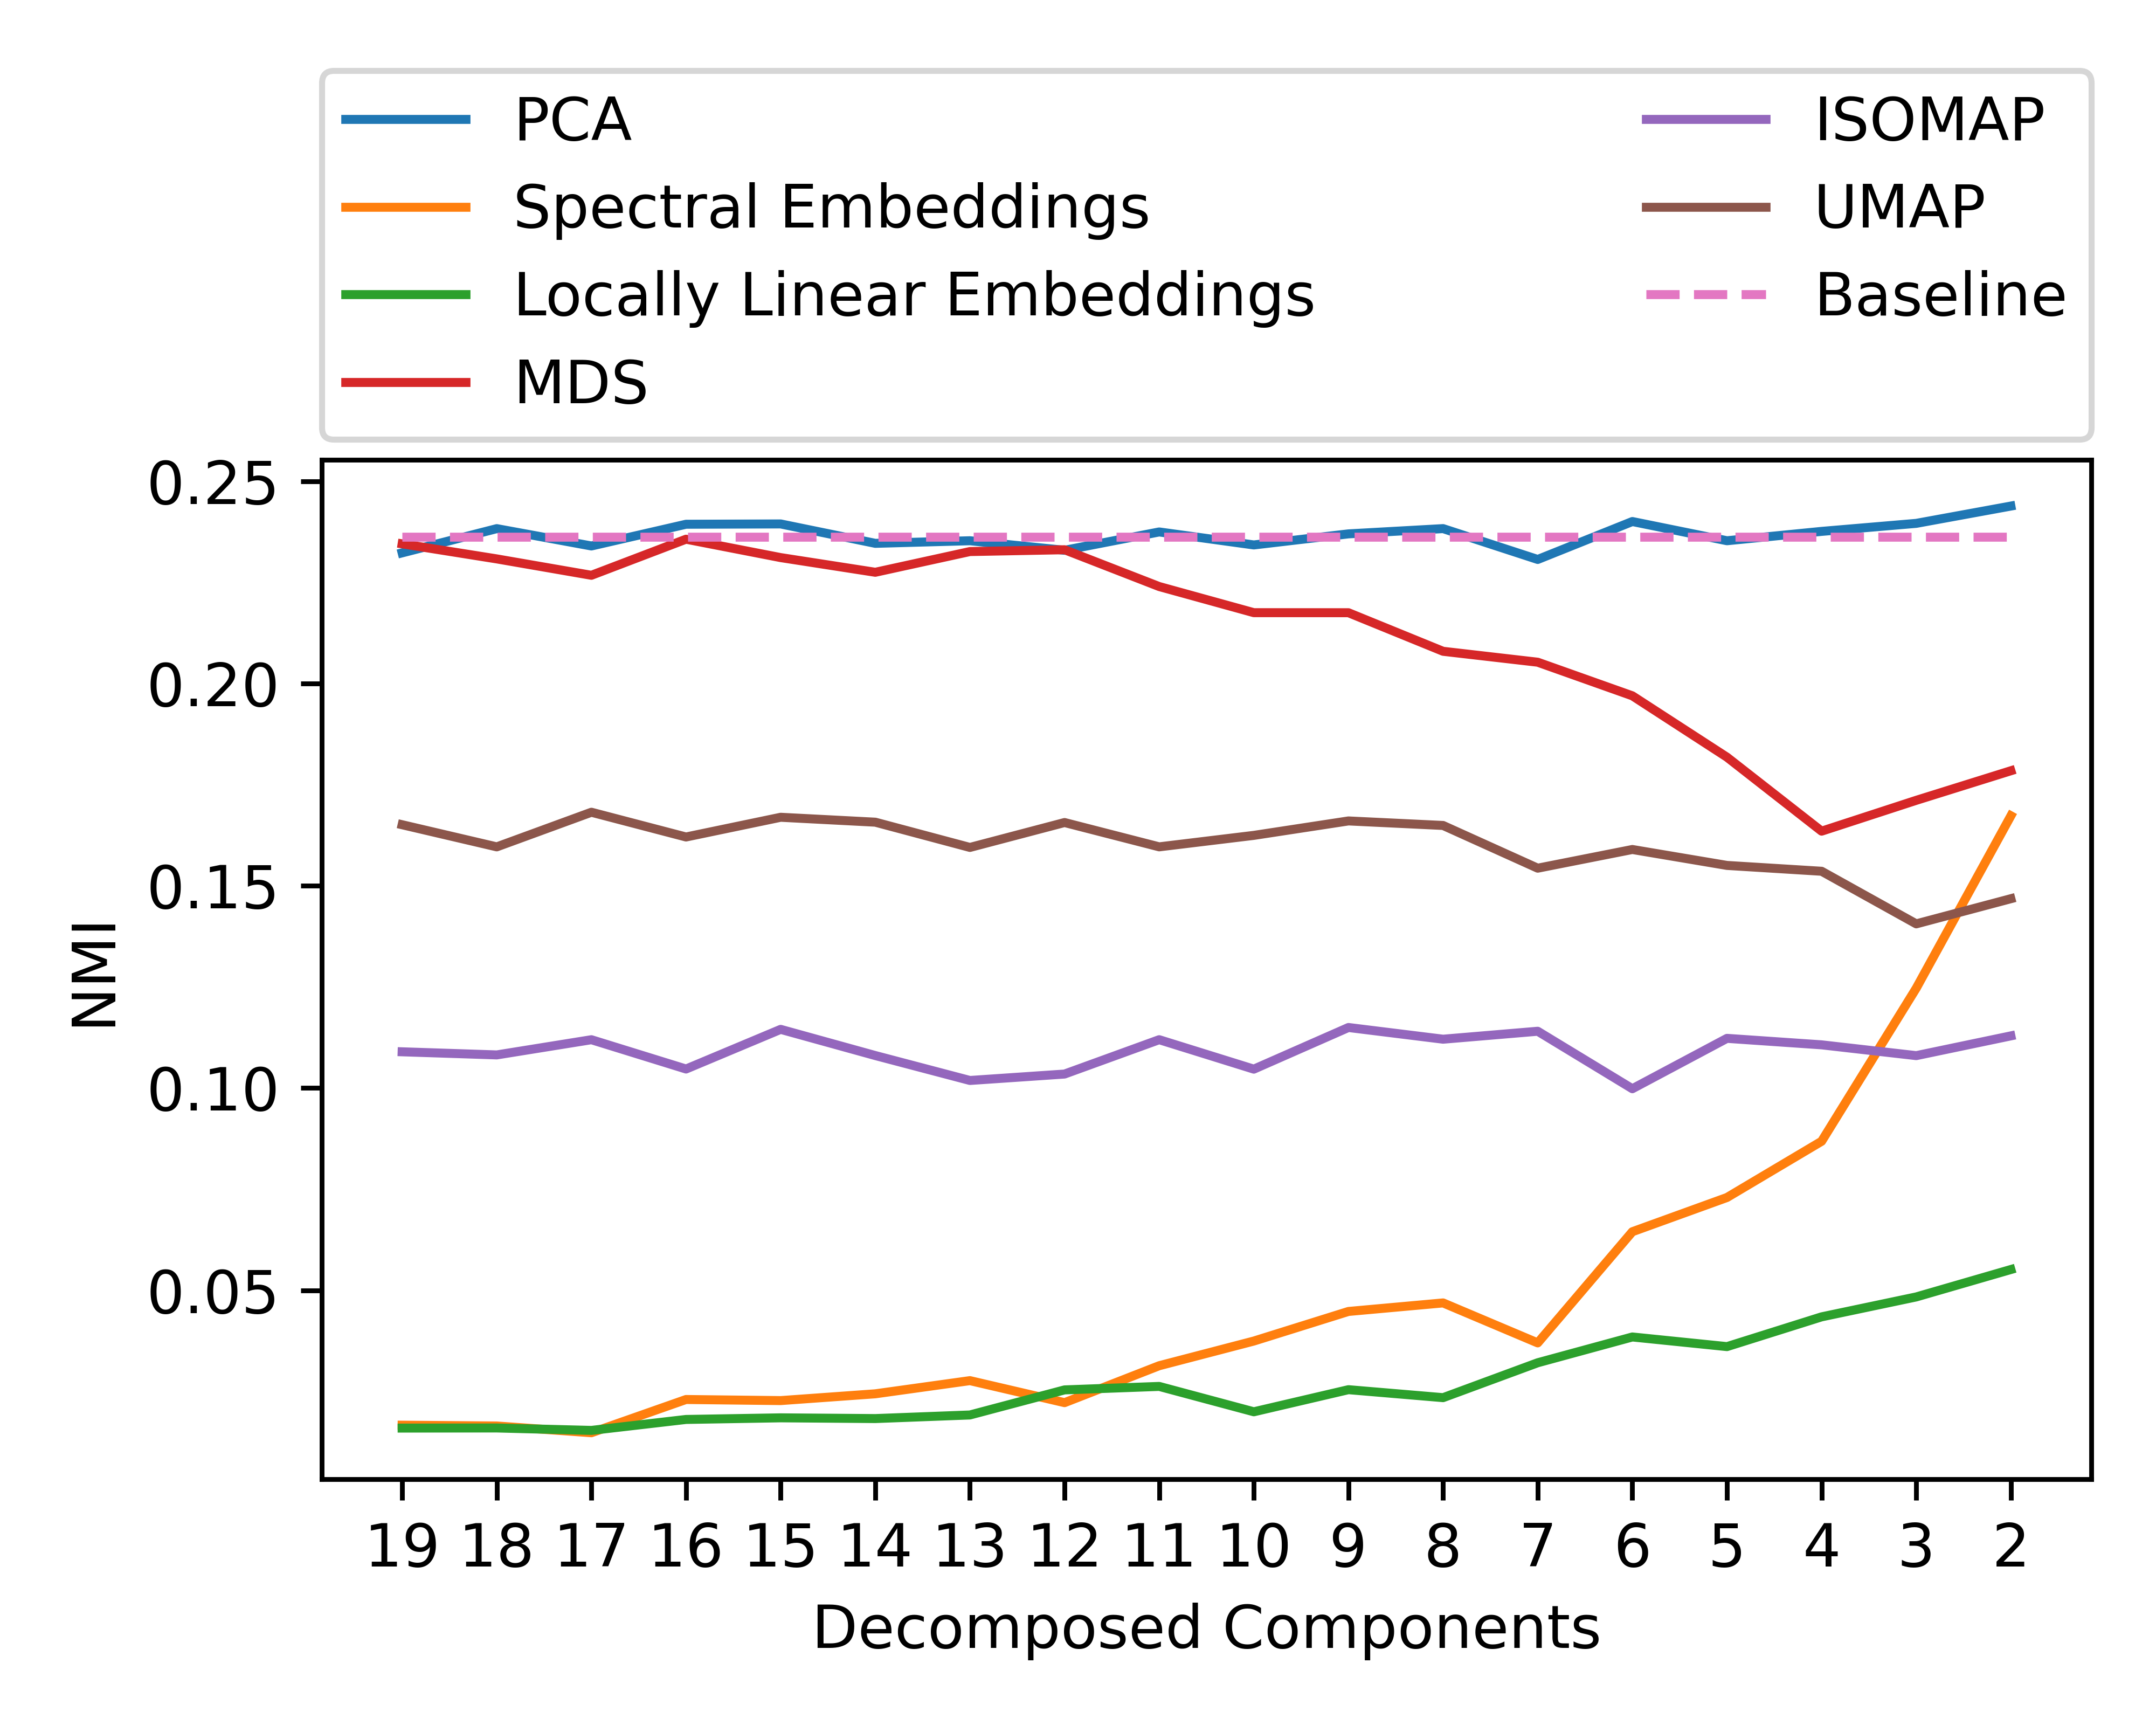
\includegraphics[width=0.48\linewidth]{images/charts/detailed_decomposition_metric_t_0.8_p_2_comparison_2_clusters_nmi.png}
                    \label{subfig:synthetic:t_0.8:dim_influence:nmi}
                }
                \subfigure[]{
                    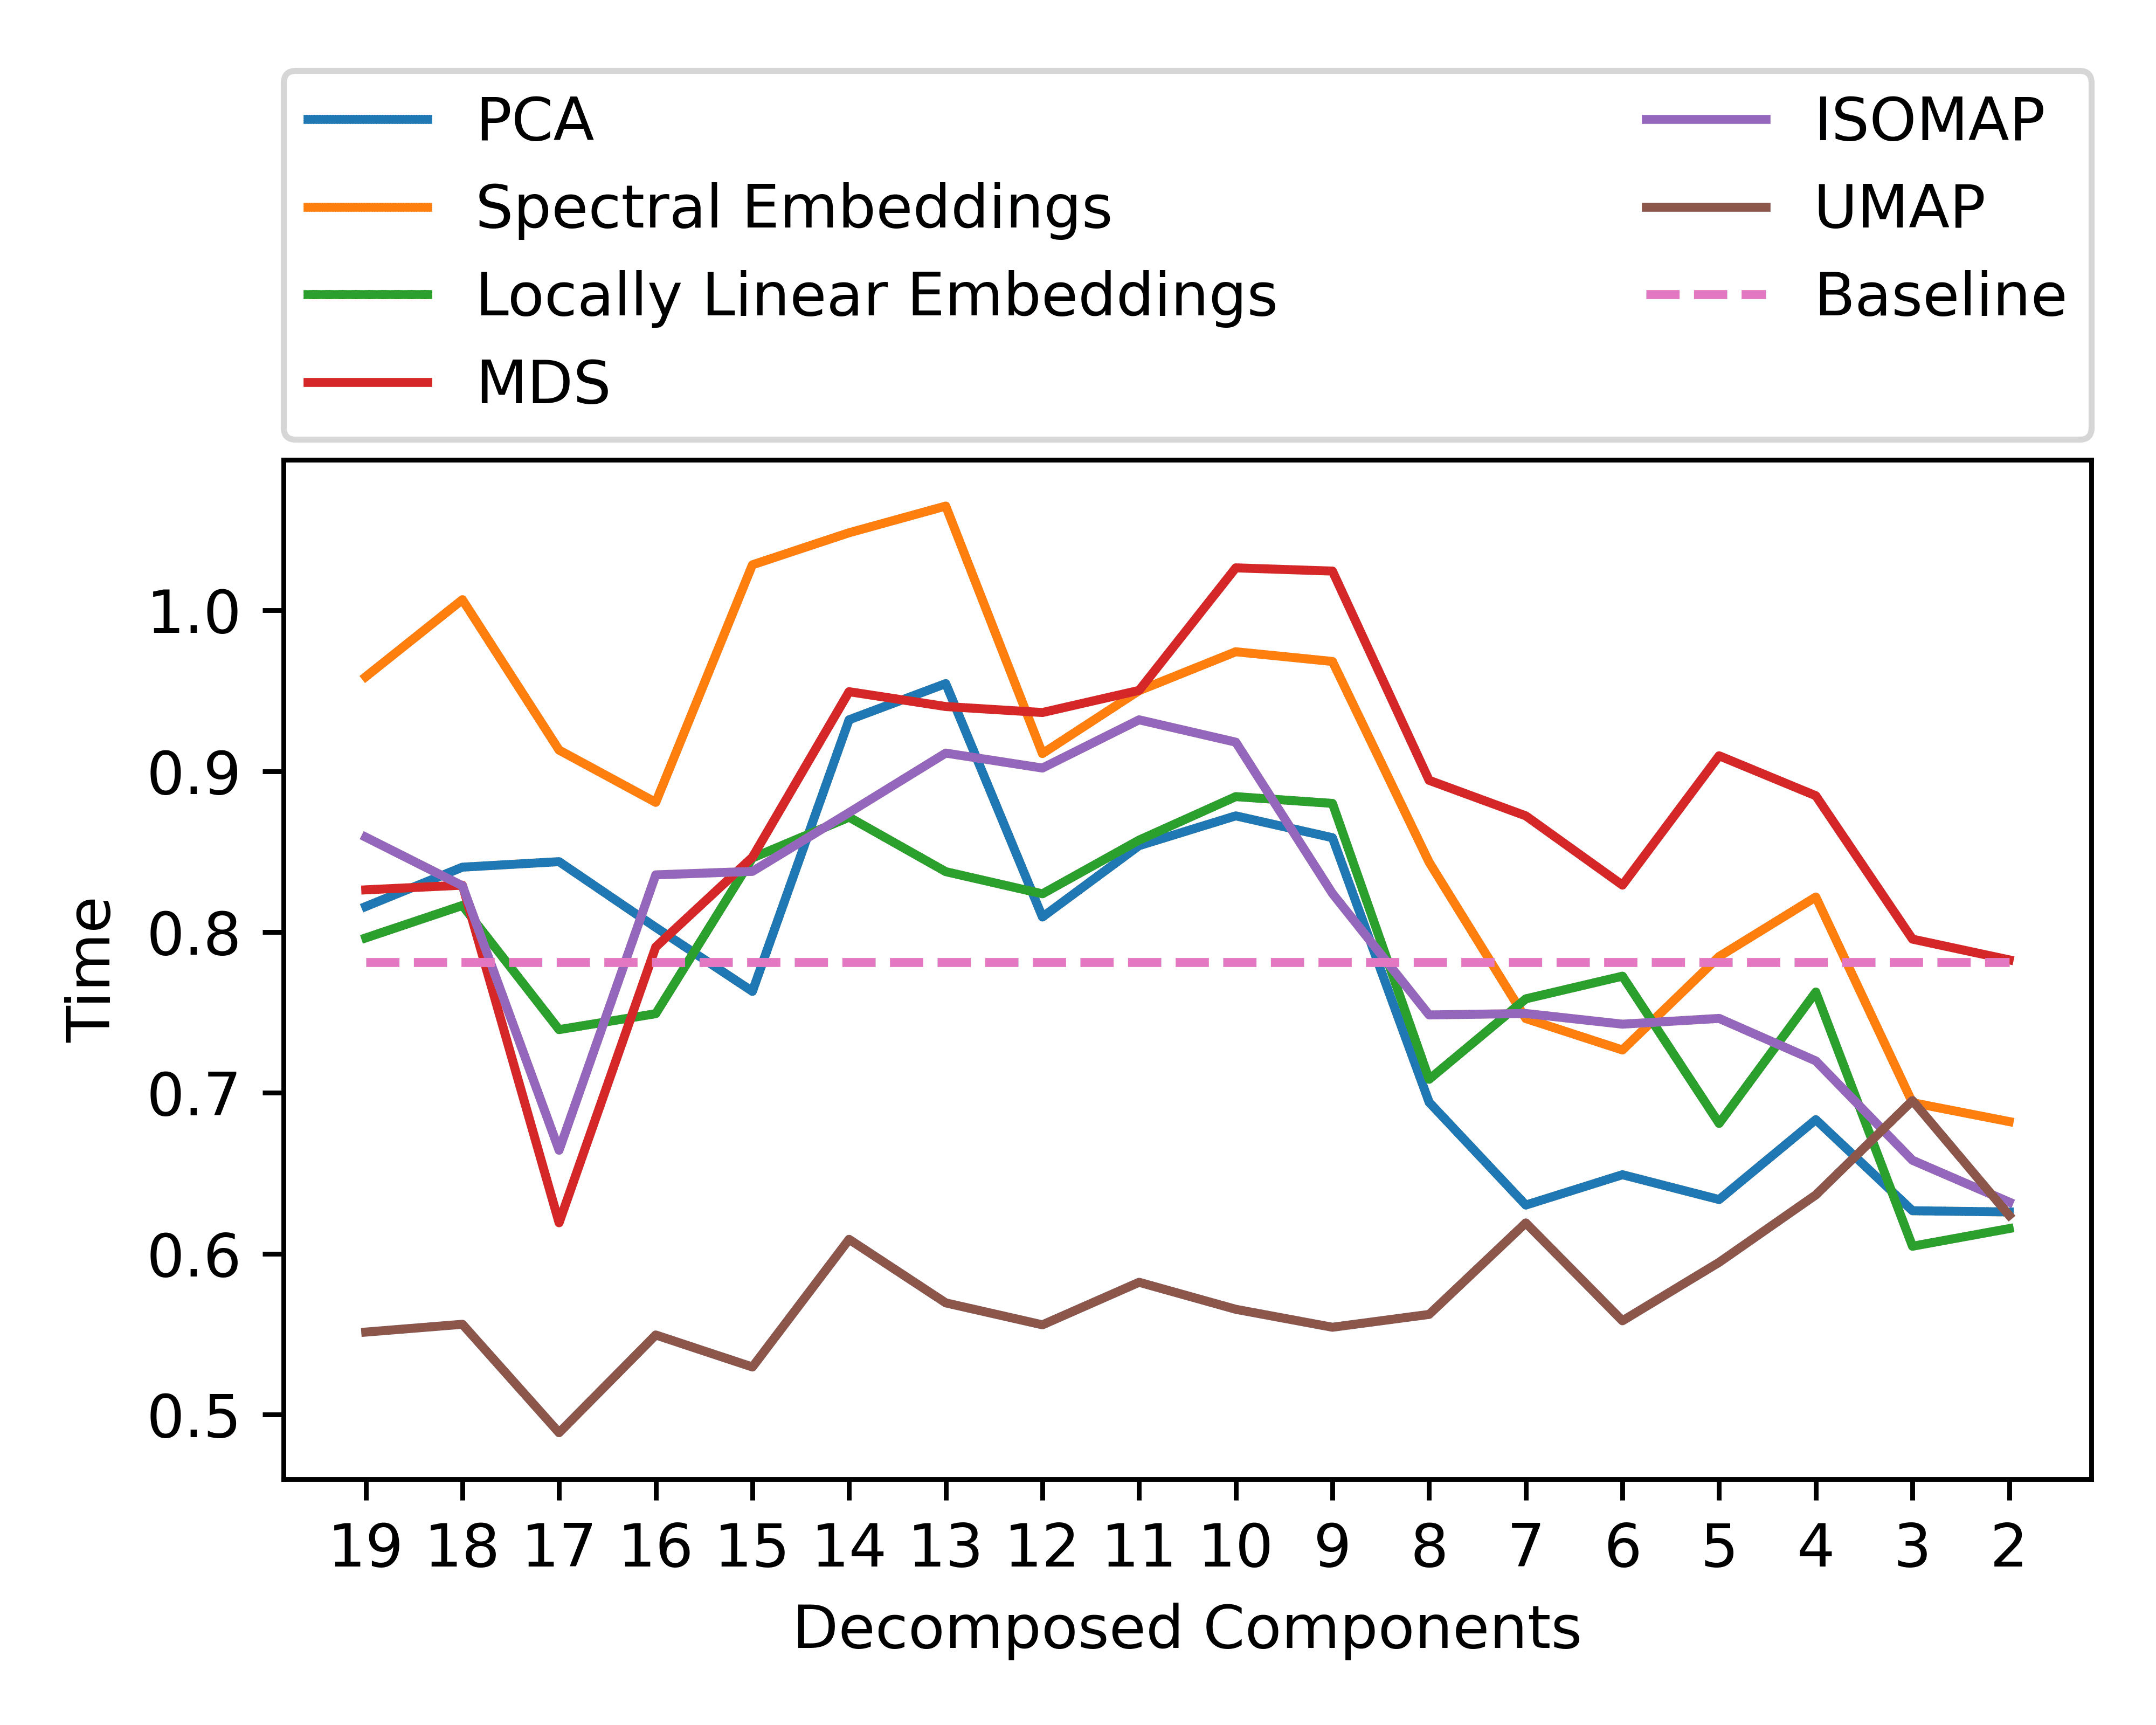
\includegraphics[width=0.48\linewidth]{images/charts/detailed_decomposition_metric_t_0.8_p_2_comparison_2_clusters_time.png}
                    \label{subfig:synthetic:t_0.8:dim_influence:time}
                }
                \caption{Анализ влияния размерности данных при различных методах снижения размерности на кластеризацию синтетического набора данных с параметром \(t = 0.8\). Линия Baseline -- результат работы алгоритма \kmeans{} без предварительного снижения размерности. Результаты для
                    \subref{subfig:synthetic:t_0.8:dim_influence:ami} AMI;
                    \subref{subfig:synthetic:t_0.8:dim_influence:ari} ARI;
                    \subref{subfig:synthetic:t_0.8:dim_influence:nmi} NMI, а также на время работы алгоритма \subref{subfig:synthetic:t_influence:time}.
                }
                \label{fig:synthetic:t_0.8:dim_influence}
            \end{figure}

            Таким образом, эксперимент подтвердил, что даже в условиях идеальной геометрии кластеров агрессивное снижение размерности способно существенно нарушить пространственную структуру, необходимую для корректной работы \kmeans{}. Наиболее устойчивыми к снижению размерности оказались методы PCA и MDS. Это подчеркивает важность выбора метода снижения размерности в зависимости от допустимой степени искажения данных при сохранении кластерной структуры.

        \subsubsection{Анализ поведения методов снижения кластеризации при сближении кластеров}
            В данной части экспериментов особое внимание уделяется анализу устойчивости и адаптивности различных методов снижения размерности в условиях, когда кластеры в данных становятся все менее различимыми -- то есть постепенно сближаются в пространстве признаков. Синтетическая модель, построенная как смесь нормальных распределений с контролируемым расстоянием между центрами кластеров, позволяет формализованно варьировать степень перекрытия кластеров с помощью параметра \(t\), не изменяя другие характеристики выборки.

            В условиях, когда \(t < 0\), центры кластеров максимально удаляются друг от друга без пересечений, что соответствует идеальному случаю для алгоритма \kmeans{}. По мере увеличения значения \(t\) до \(1\) центры притягиваются к общему центру масс, и границы между кластерами становятся все менее четкими, что моделирует реальные сценарии, в которых классы могут частично перекрываться. Такой подход позволяет объективно оценить, насколько методы понижения размерности сохраняют или теряют разделимость между группами при убывающем межкластерном расстоянии.

            Результаты экспериментов продемонстрированы на рисунке \ref{fig:synthetic:t_influence}, и показали высокую степень чувствительности к росту перекрытия кластеров.

            При анализе показателей AMI, ARI и NMI можно наблюдать устойчивое превосходство методов MDS, ISOMAP и UMAP на всех значениях параметра \(t\), особенно в областях, где кластеры хорошо разделены (\(t < 0.4\)). Эти методы демонстрируют почти идеальное восстановление кластерной структуры при низких значениях \(t\), что соответствует высокой степени отделенности кластеров. С увеличением \(t\) все методы, за исключением Spectral Embeddings и Locally Linear Embeddings (LLE), относительно стабильно теряют качество, однако сохраняют приемлемый уровень информативности вплоть до \(t \approx 0.6\). В то же время, методы Spectral и LLE показывают значительно худшие показатели на всех интервалах \(t\), демонстрируя явную нестабильность и уязвимость к изменению межкластерного расстояния.

            Особенно интересным является пик значений метрик (в районе \(t = 0.4\)) для Spectral и LLE, что может быть обусловлено локальным улучшением связности графов при частичном сближении кластеров. Однако после этого значения происходит резкое падение метрик, особенно AMI и NMI, указывающее на неспособность этих методов сохранять глобальную структуру данных при сильном перекрытии.

            С точки зрения времени выполнения, наименее ресурсоемким методом оказался UMAP, продемонстрировавший значительное снижение времени работы алгоритма кластеризации в пространстве меньшей размерности. Методы PCA, Spectral Embeddings, Locally Linear Embeddings, MDS, ISOMAP, напротив, показали увеличение времени работы при переходе в пространство меньше размерности (до 8 компонент), однако в пространствах размерности меньше 8, методы PCA, Locally Linear Embeddings, ISOMAP, продемонстрировали снижение времени работы алгоритма кластеризации, что делает их особенно предпочтительными для задач, требующих баланса между точностью и скоростью.

            Таким образом, в условиях постепенно сближающихся кластеров методы PCA, MDS и UMAP оказываются наиболее надежными как по качеству кластеризации, так и по вычислительным затратам. Методы Spectral Embeddings и Locally Linear Embeddings, напротив, показали нестабильное поведение и склонность к деградации качества при увеличении параметра \(t\).

            \begin{figure}[H]\centering
                \subfigure[]{
                    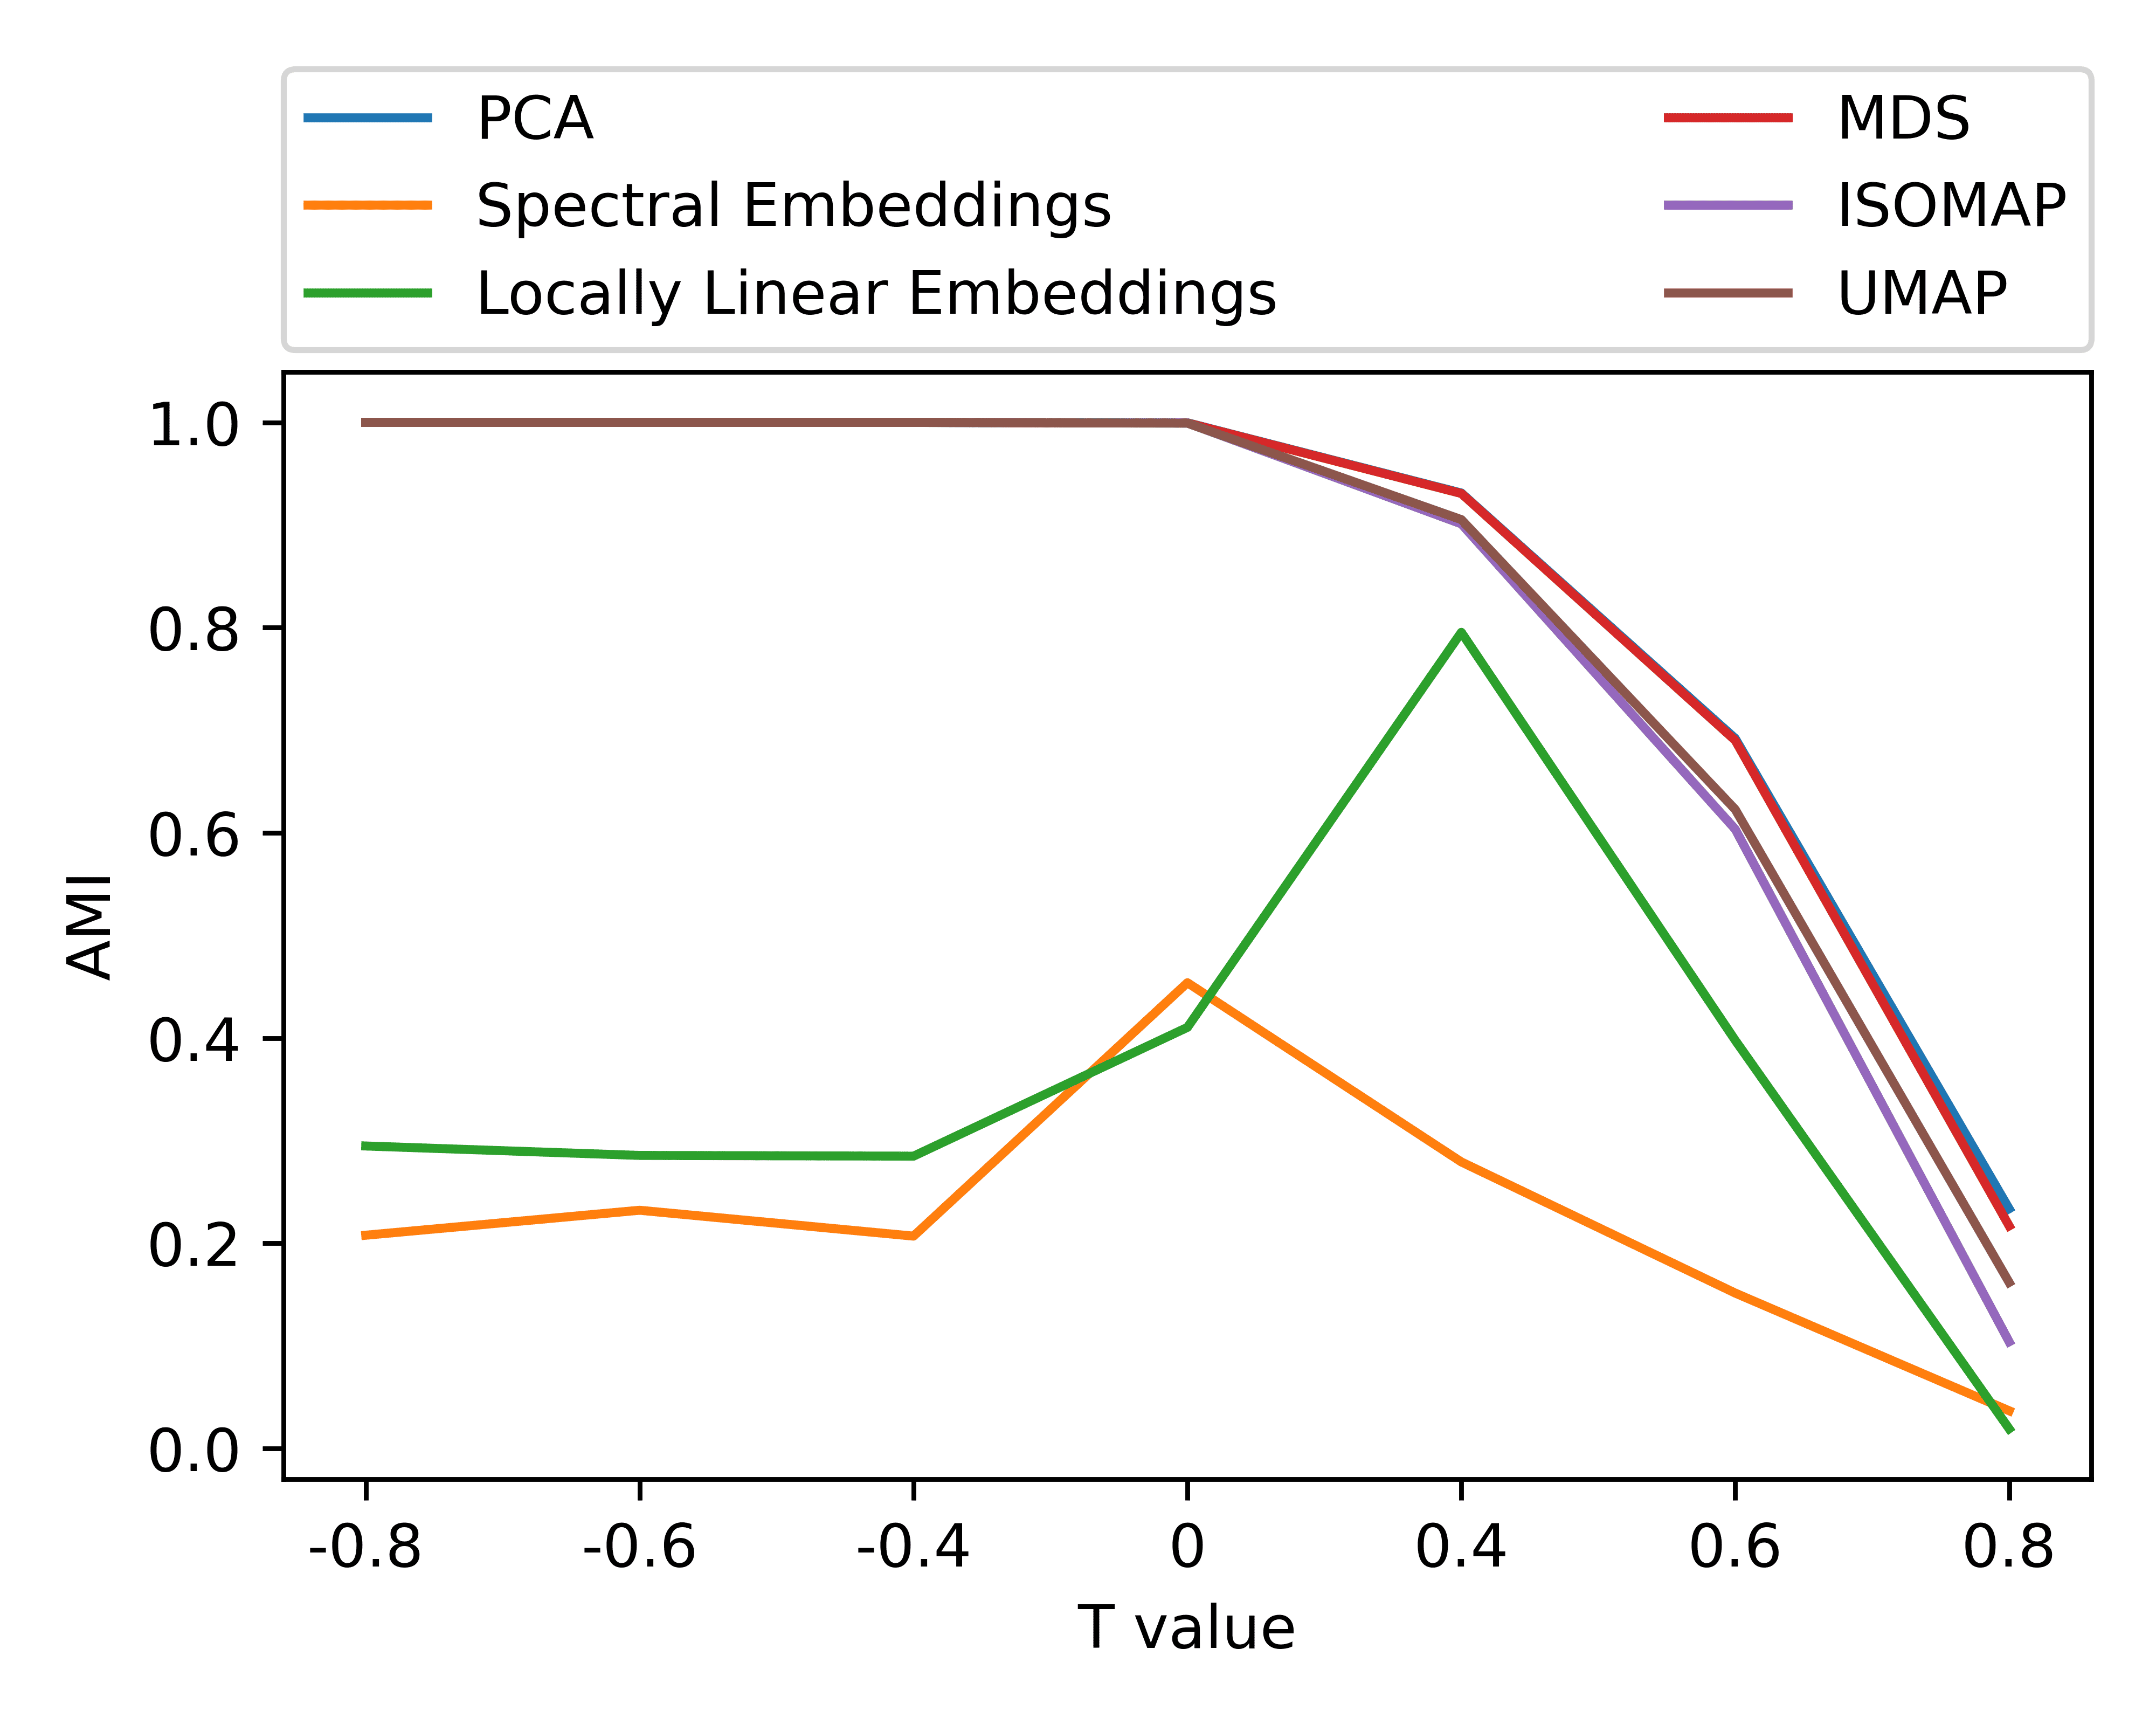
\includegraphics[width=0.48\linewidth]{images/charts/t_comparison_decomposition_20_p_2_comparison_2_clusters_ami.png}
                    \label{subfig:synthetic:t_influence:ami}
                }
                \subfigure[]{
                    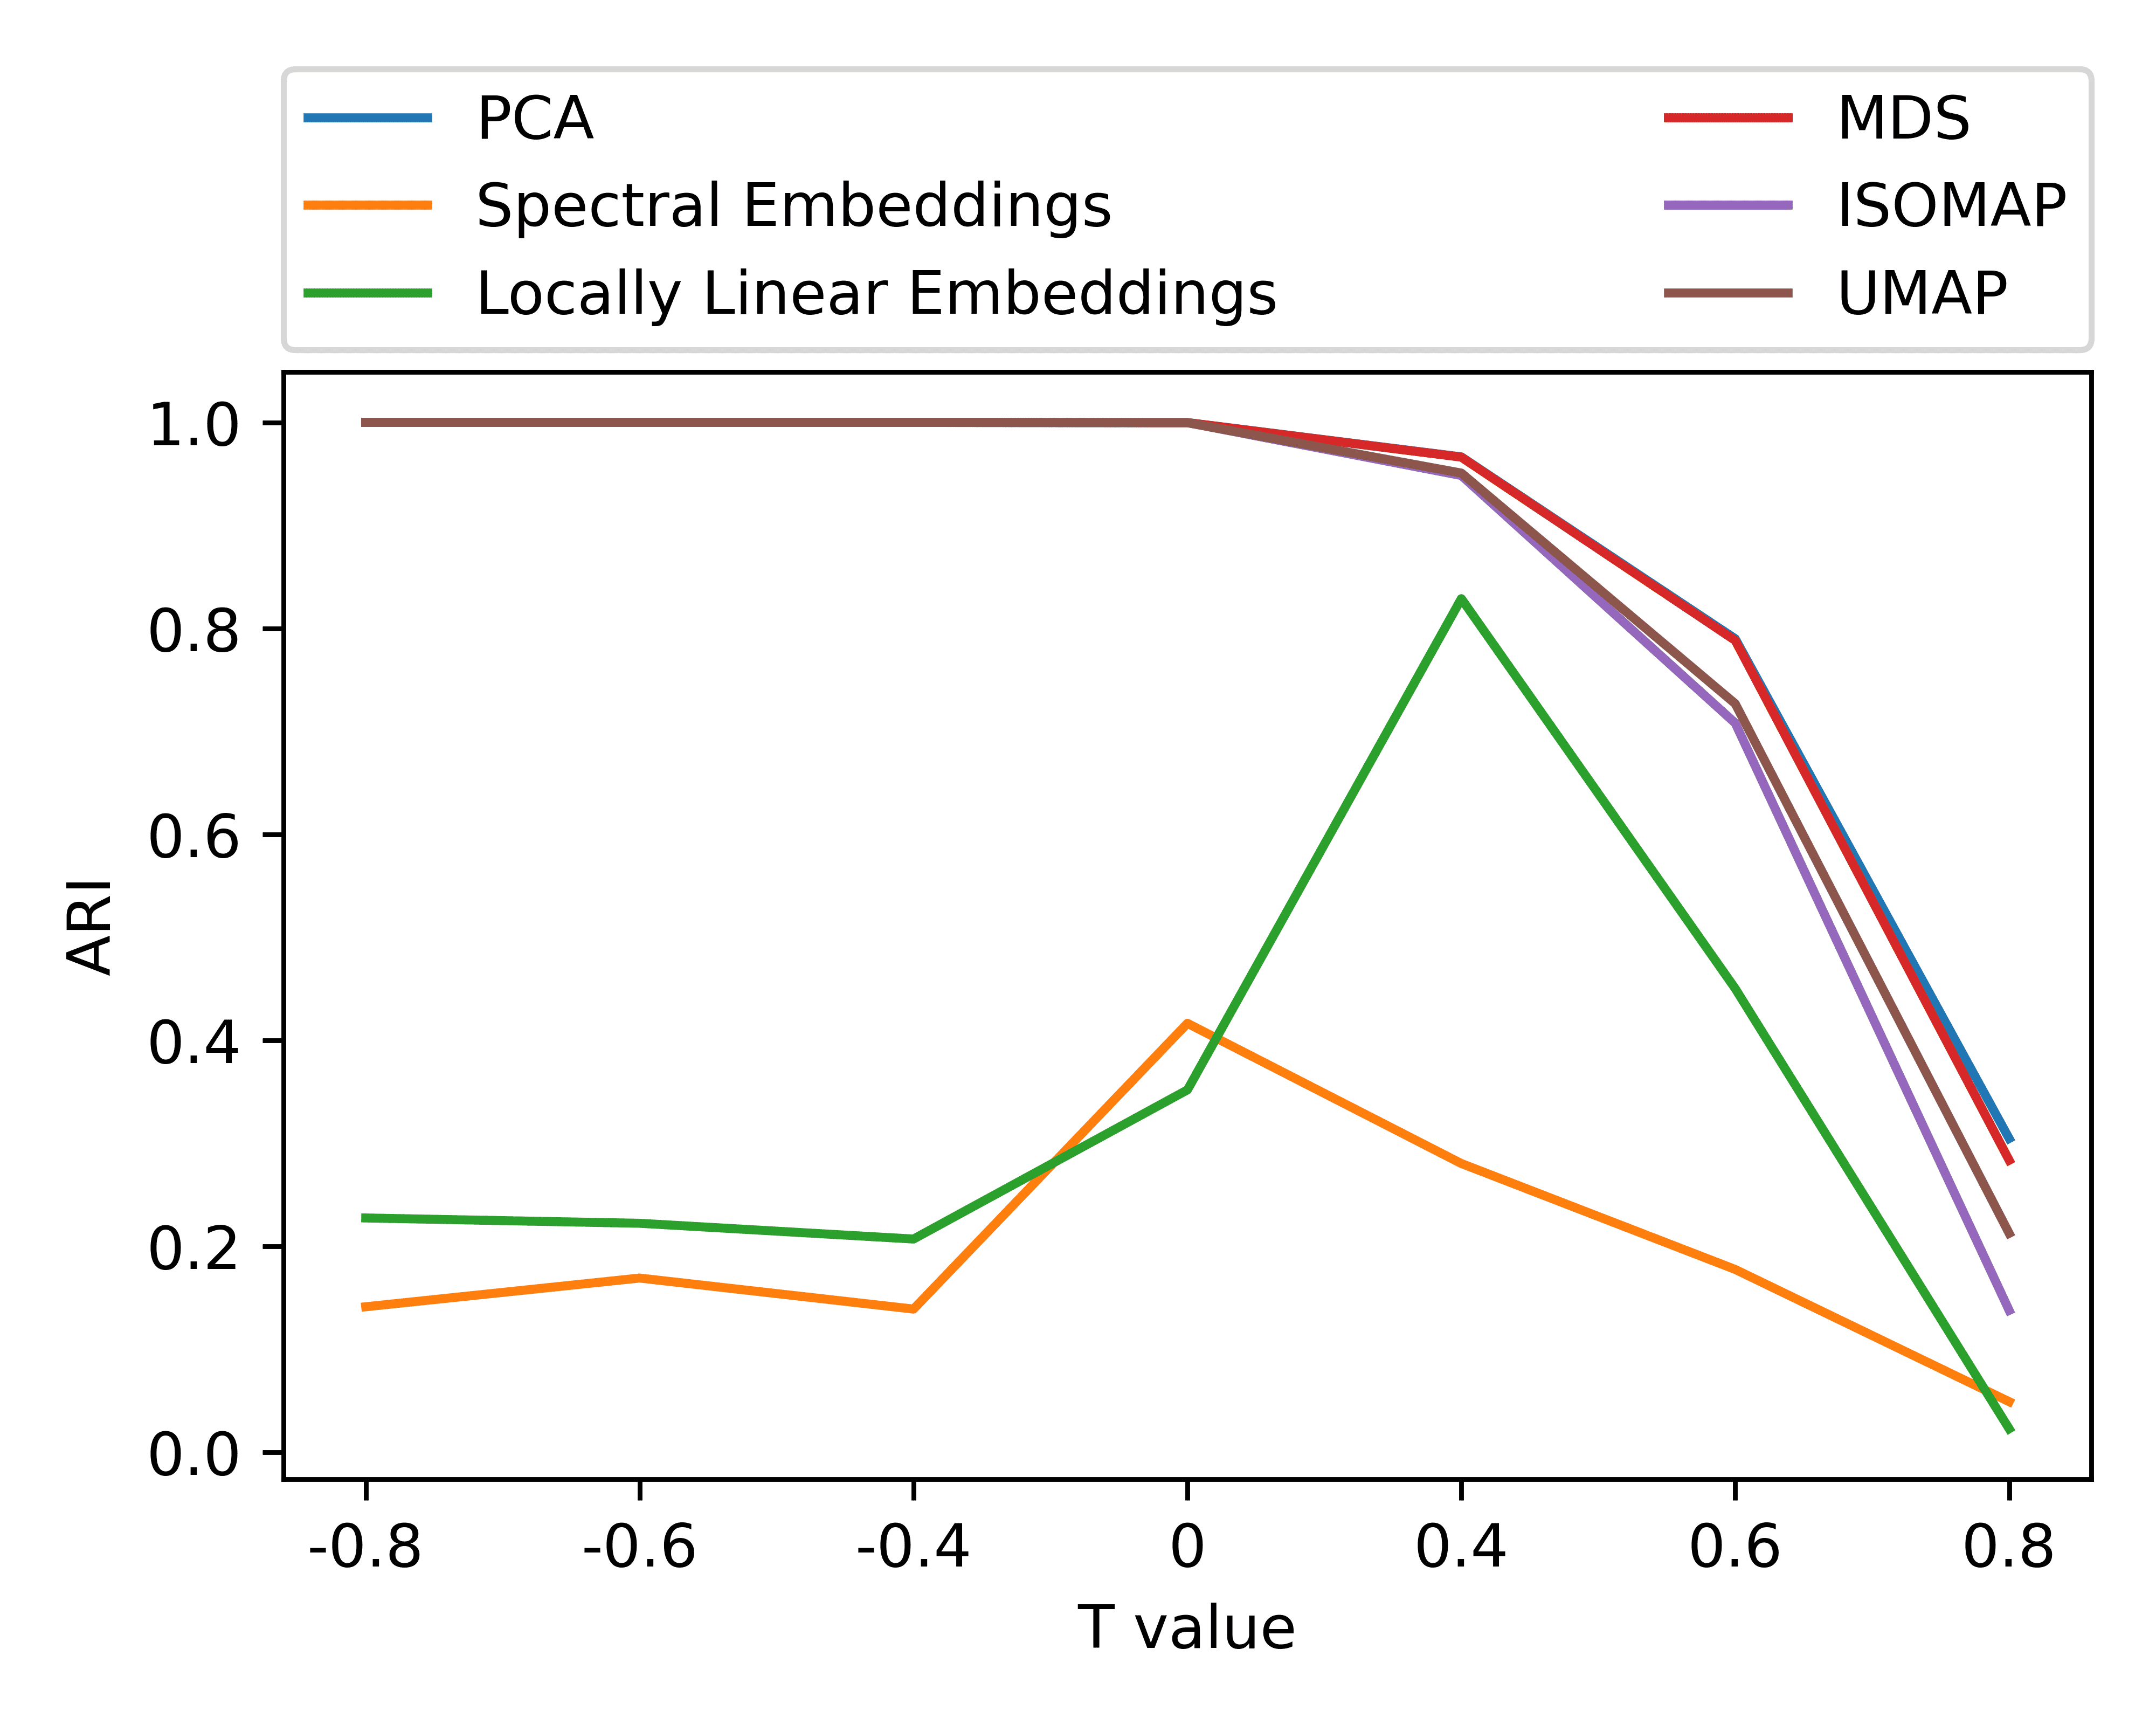
\includegraphics[width=0.48\linewidth]{images/charts/t_comparison_decomposition_20_p_2_comparison_2_clusters_ari.png}
                    \label{subfig:synthetic:t_influence:ari}
                }
                \subfigure[]{
                    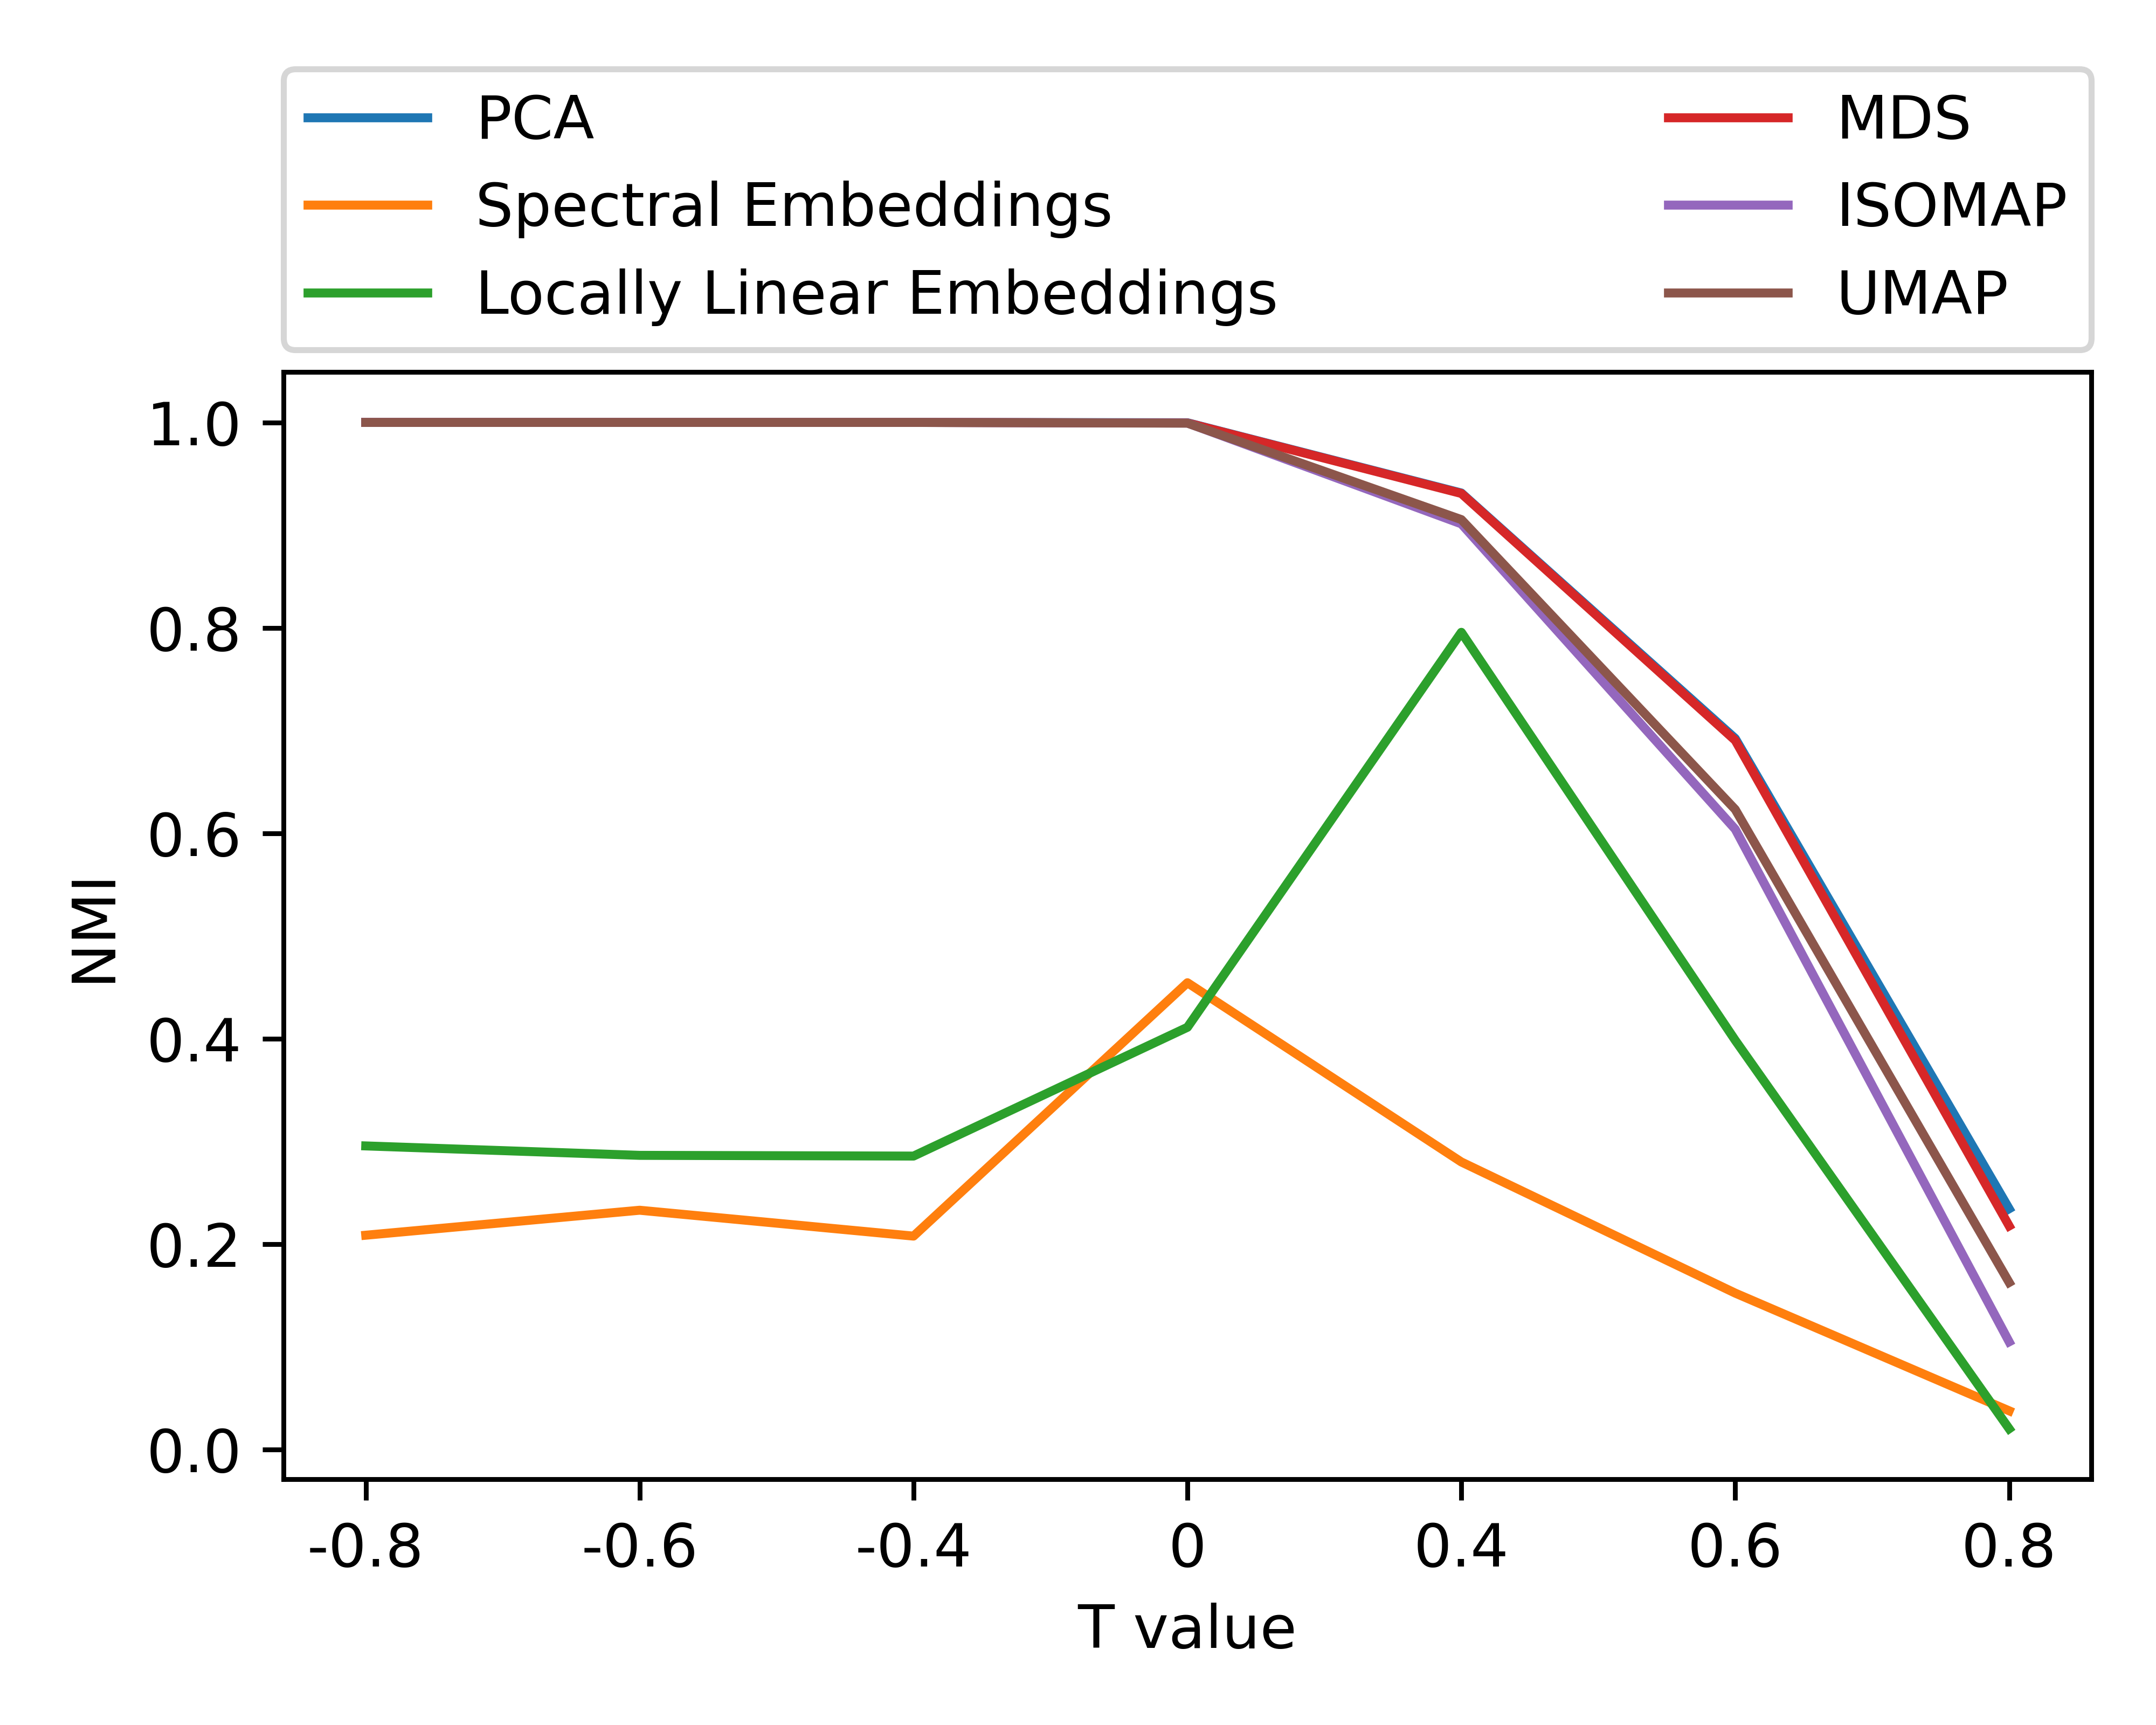
\includegraphics[width=0.48\linewidth]{images/charts/t_comparison_decomposition_20_p_2_comparison_2_clusters_nmi.png}
                    \label{subfig:synthetic:t_influence:nmi}
                }
                \subfigure[]{
                    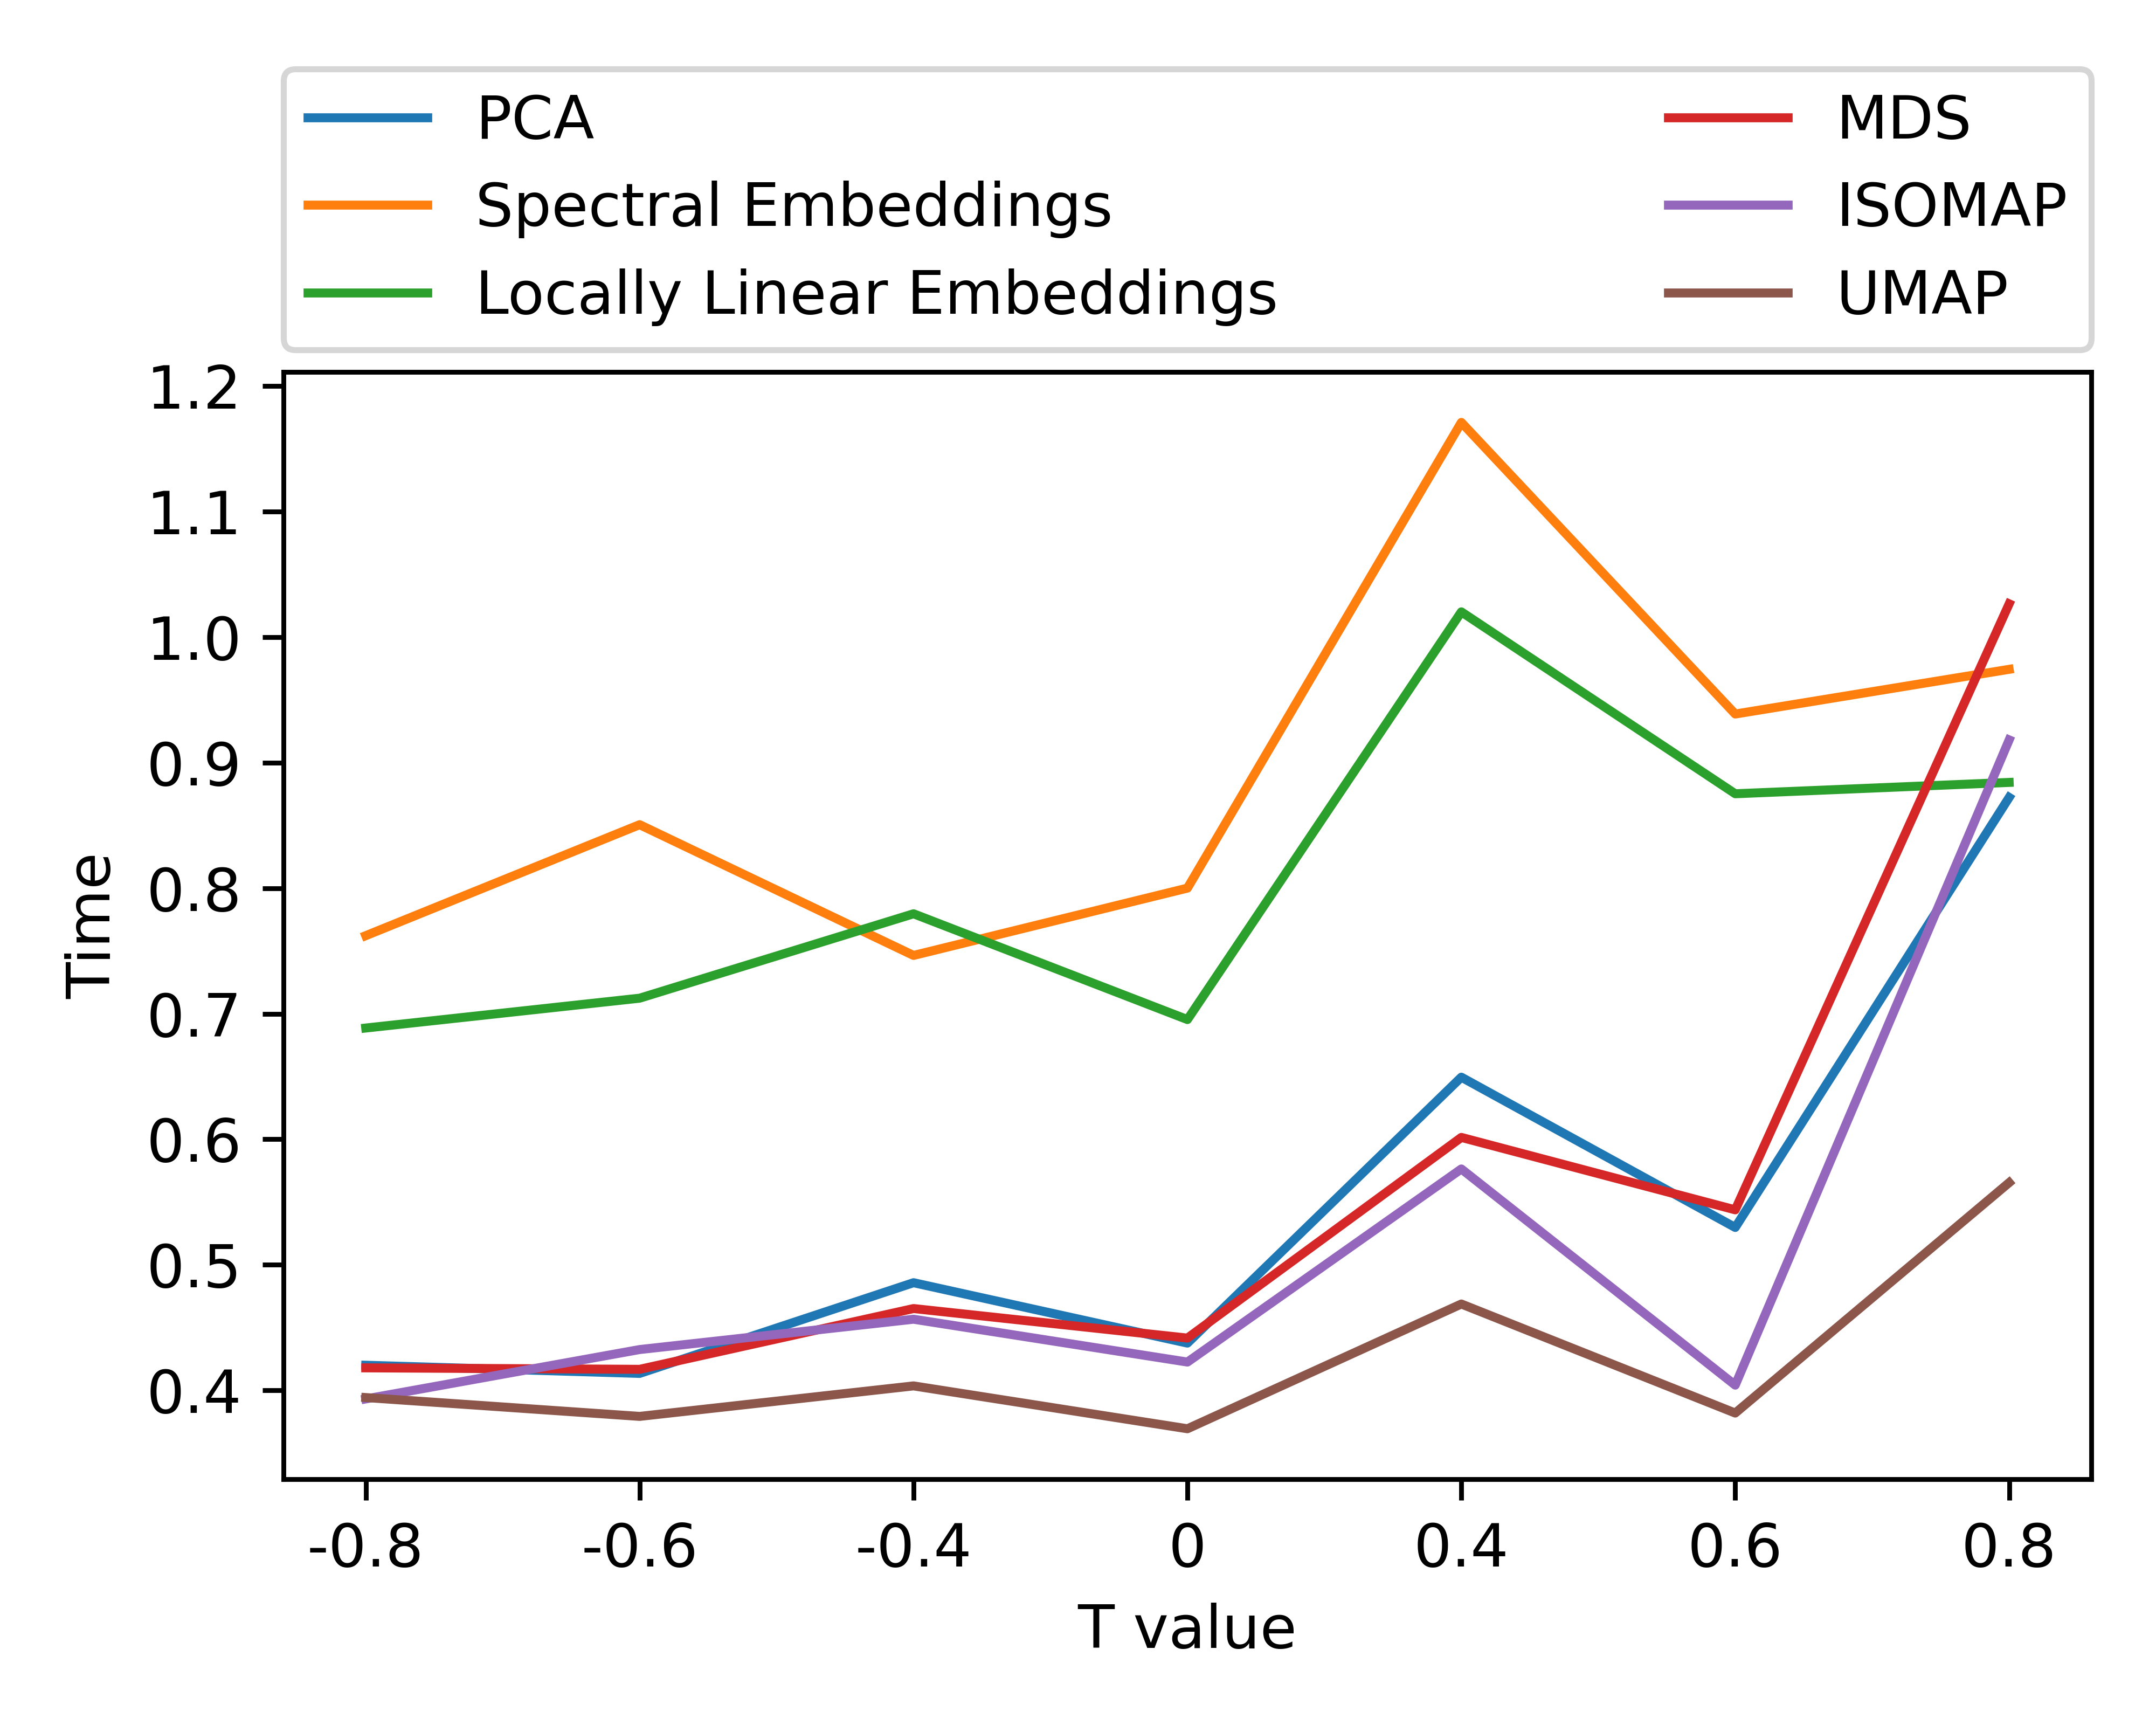
\includegraphics[width=0.48\linewidth]{images/charts/t_comparison_decomposition_20_p_2_comparison_2_clusters_time.png}
                    \label{subfig:synthetic:t_influence:time}
                }
                \caption{Анализ влияния различных методов снижения размерности данных на кластеризацию синтетического набора данных при сближении и отдалении центров кластеров. Результаты для
                    \subref{subfig:synthetic:t_influence:ami} AMI;
                    \subref{subfig:synthetic:t_influence:ari} ARI;
                    \subref{subfig:synthetic:t_influence:nmi} NMI, а также на время работы алгоритма \subref{subfig:synthetic:t_influence:time}.
                }
                \label{fig:synthetic:t_influence}
            \end{figure}

            Таким образом, анализ на синтетических данных подтвердил, что эффективность методов снижения размерности сильно зависит от геометрии и плотности кластеров. Это подчеркивает необходимость адаптивного выбора метода снижения размерности в зависимости от ожидаемой сложности кластерной структуры в данных.

    \subsection{Эксперименты на реальных данных}

        Также предложенный подход был исследован на реальных данных. Для этого было решено использовать несколько стандартных наборов данных:

        \begin{itemize}
            \item Breast Cancer \cite{dataset:breastcancer},
            \item Digits \cite{dataset:digits},
            \item Wine \cite{dataset:wine}.
        \end{itemize}

        \subsubsection{Результаты алгоритма на наборе данных Breast Cancer}
            Breast Cancer -- это стандартный набор данных для бинарной классификации, часто используемый в задачах медицинской диагностики. Данные содержат результаты измерений опухолей молочной железы, полученные при помощи тонкоигольной аспирационной биопсии (FNA). Каждая запись включает характеристики клеточных ядер, такие как радиус, текстура, периметр и другие морфологические признаки.

            \begin{table}[H]
                \centering
                \caption{Характеристики набора данных Breast Cancer.}
                \begin{tabular}{ccc}
                    \toprule
                    Число классов & Число объектов & Размерность пространства \\
                    \midrule
                    2 & 569 & 30 \\
                    \bottomrule
                \end{tabular}
            \end{table}

            Набор данных Breast Cancer представляет собой матрицу размерностью 569x30, где каждая строка соответствует отдельному образцу опухоли, а каждый столбец содержит числовое значение одного из диагностических признаков. Целевая переменная указывает на доброкачественность (benign) или злокачественность (malignant) новообразования. Данные часто используются для обучения моделей машинного обучения, направленных на автоматизацию диагностики рака молочной железы.

            \begin{figure}[H]\centering
                \subfigure[]{
                    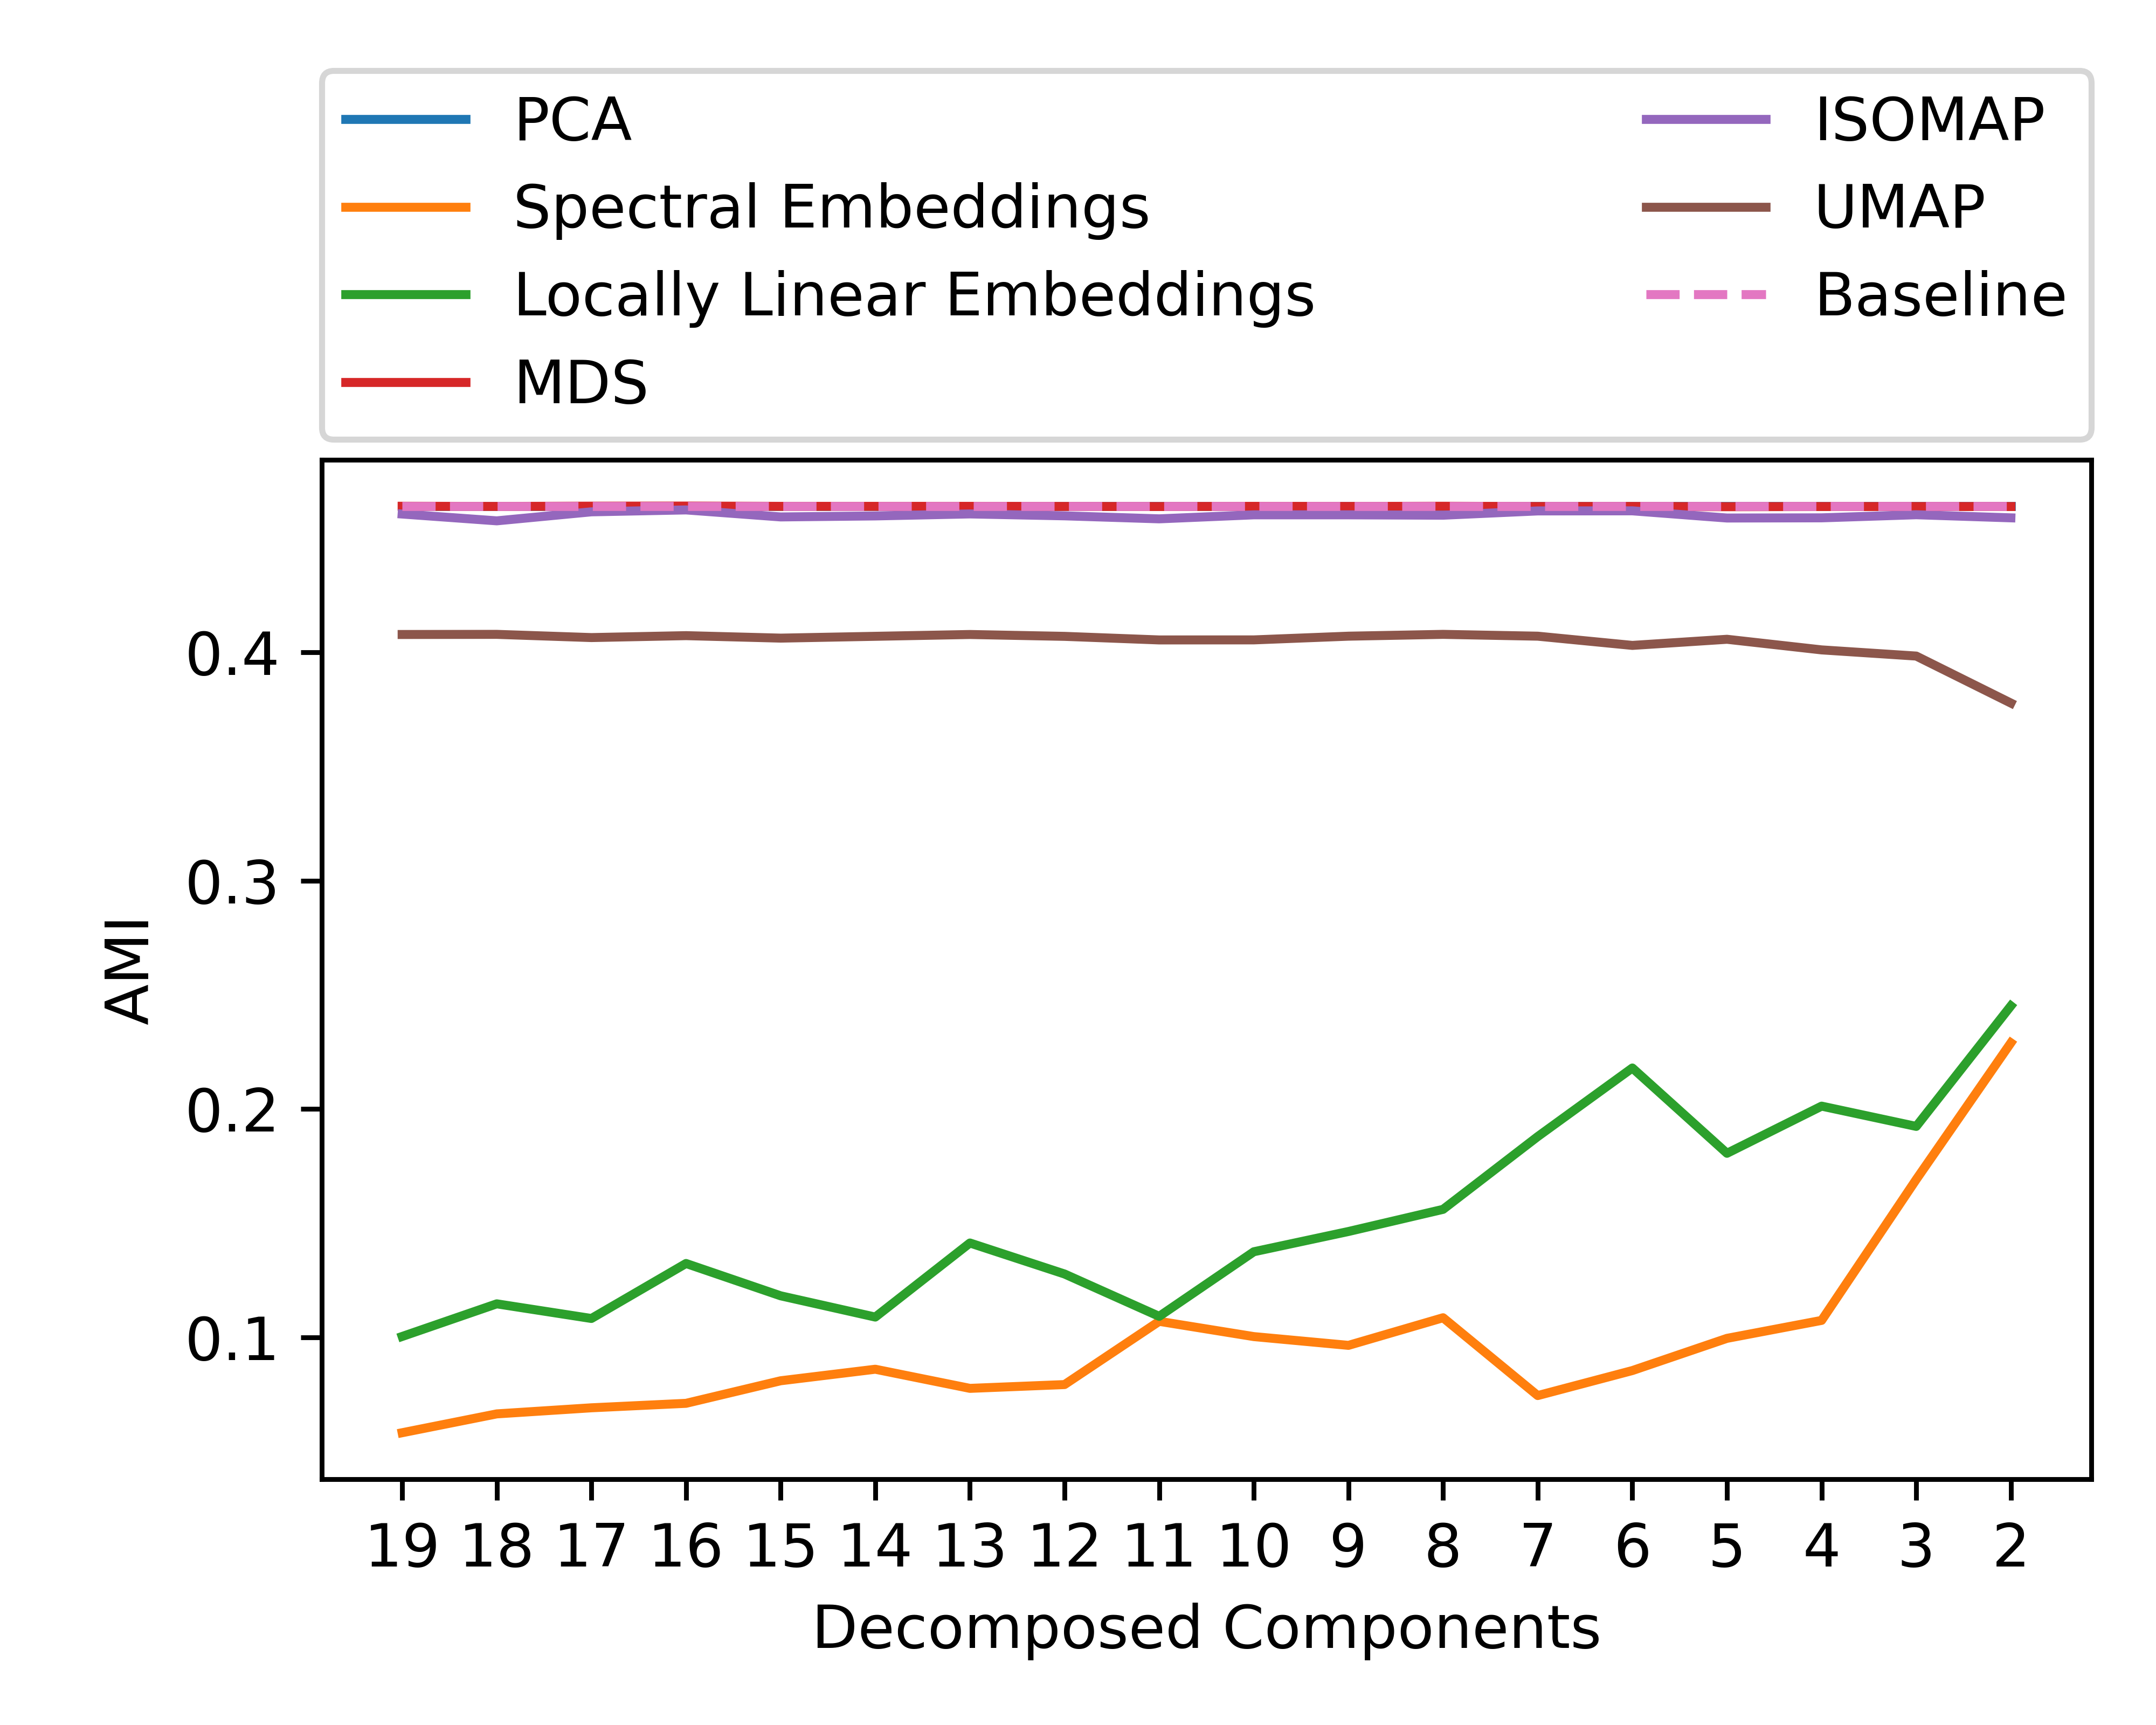
\includegraphics[width=0.48\linewidth]{images/charts_real/real_data_breast_cancer_ami.png}
                    \label{subfig:breast_cancer:ami}
                }
                \subfigure[]{
                    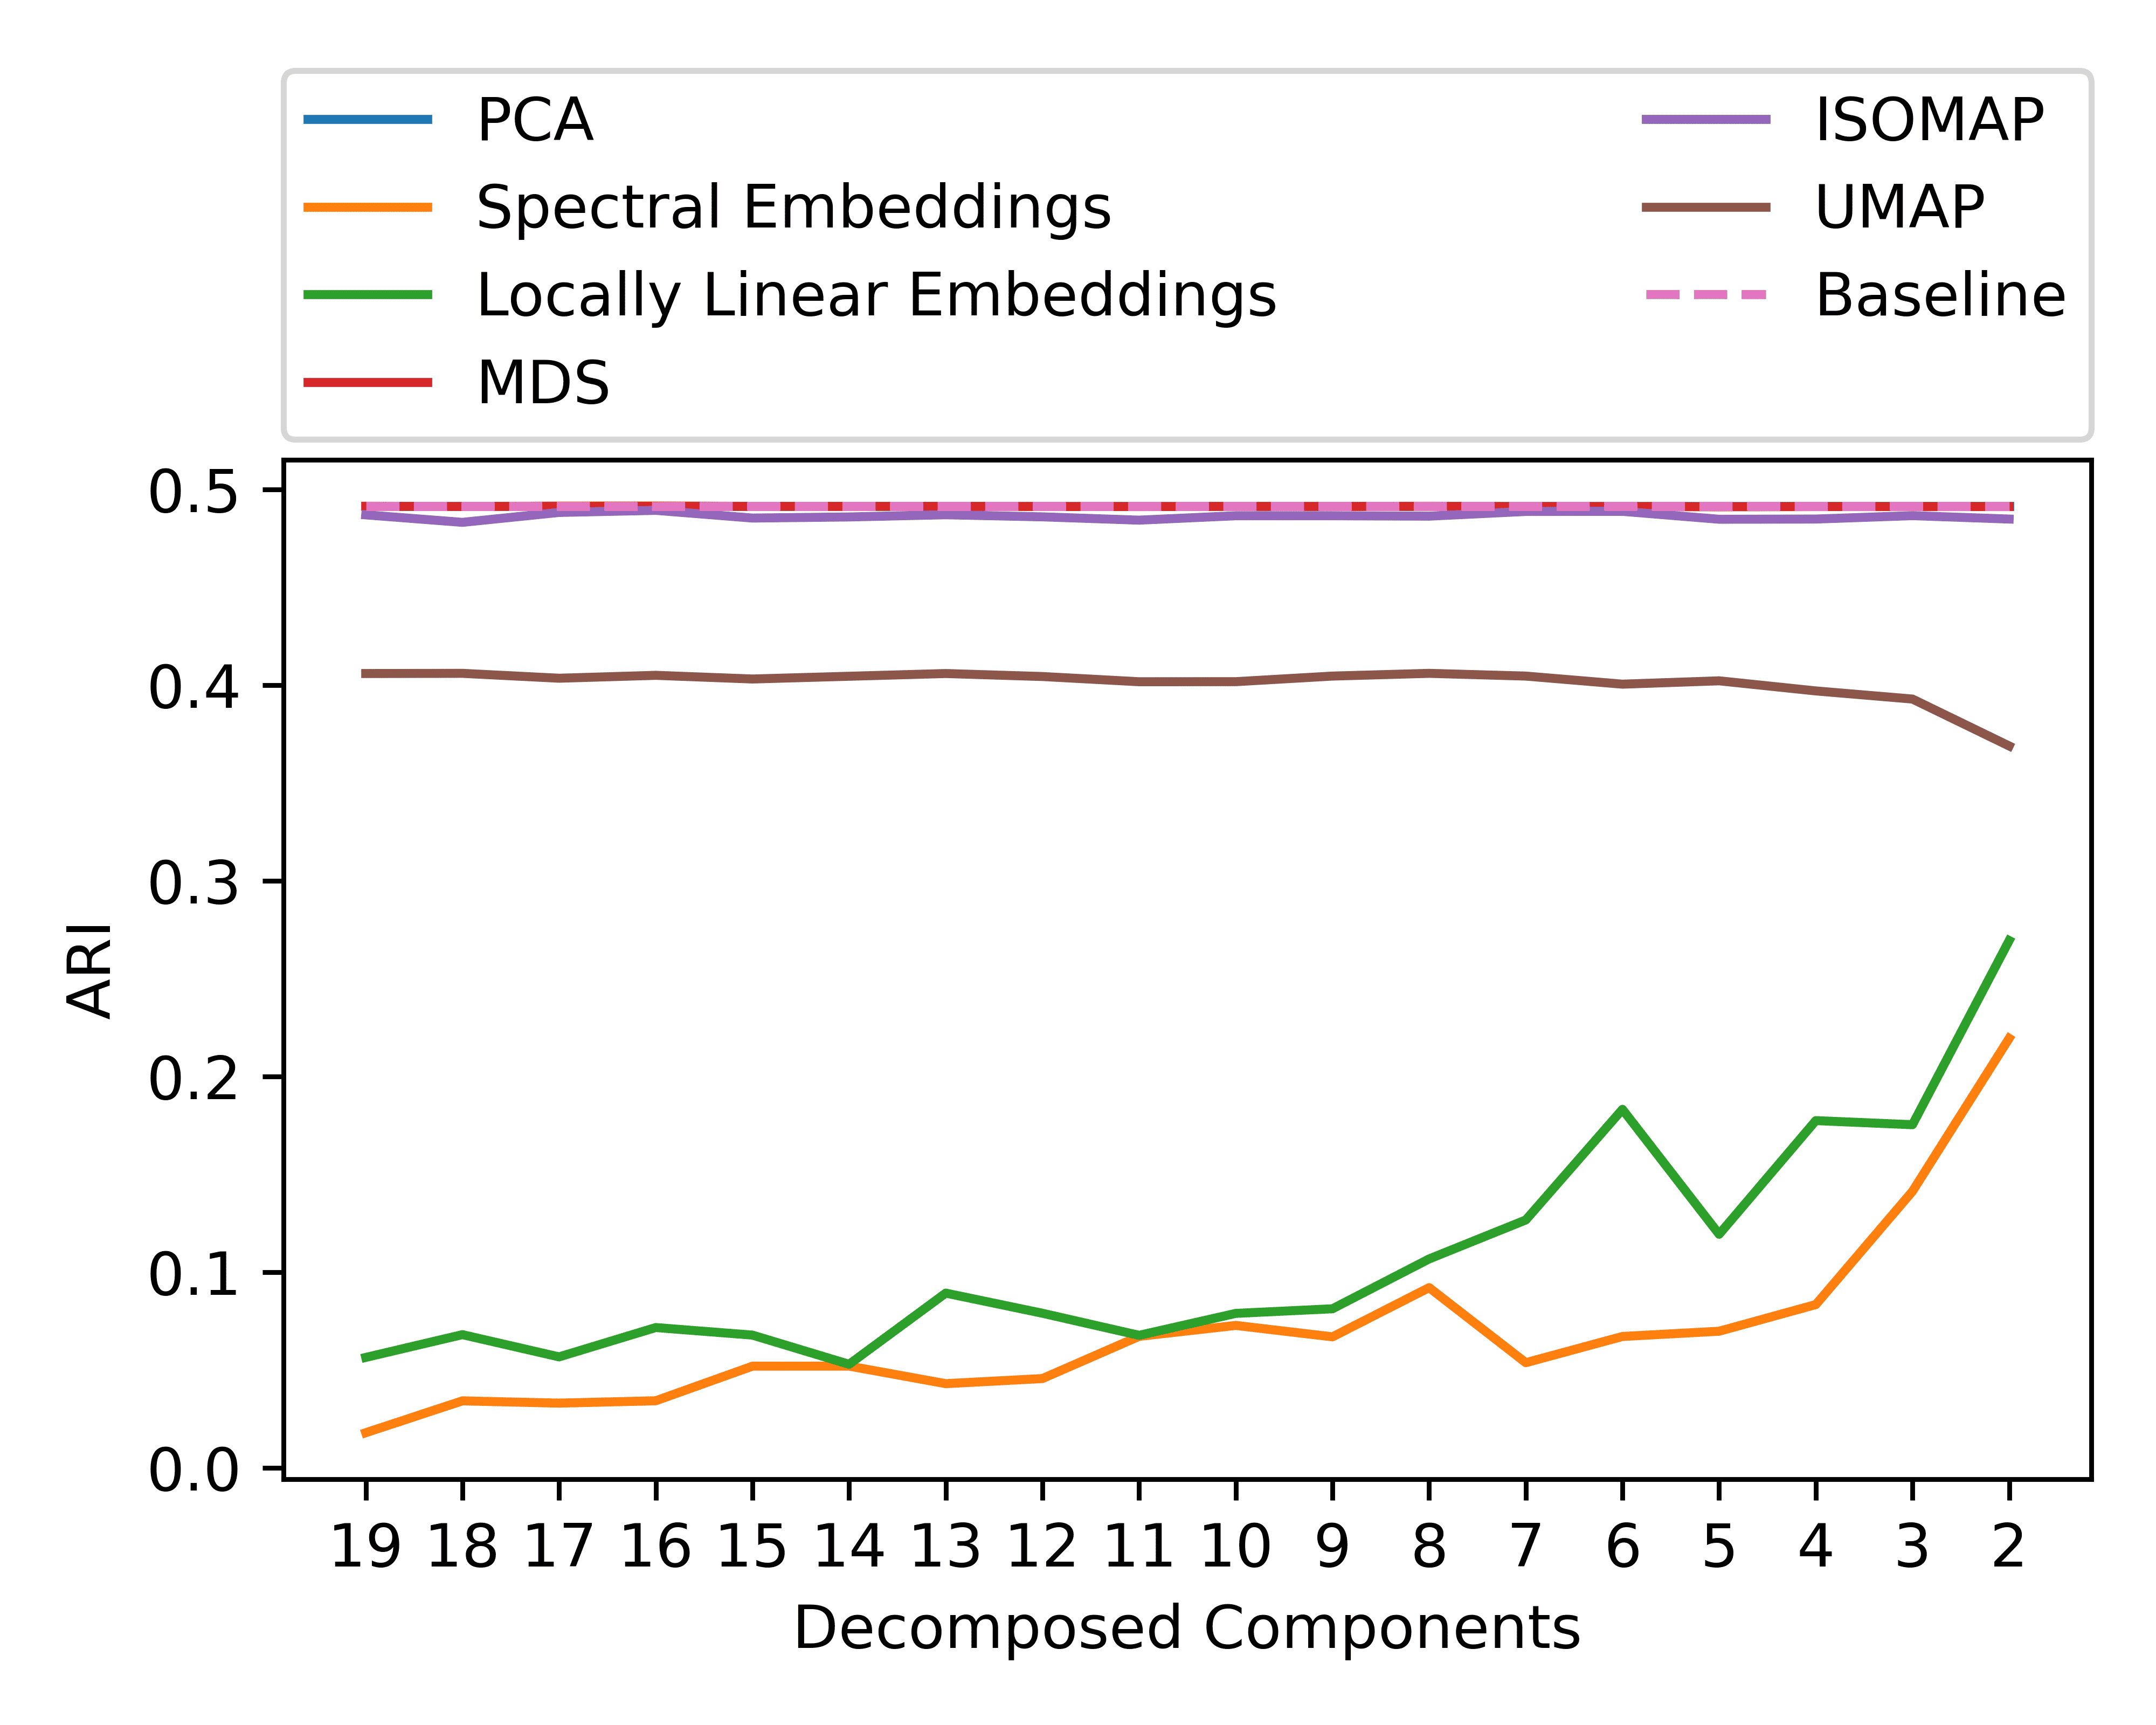
\includegraphics[width=0.48\linewidth]{images/charts_real/real_data_breast_cancer_ari.png}
                    \label{subfig:breast_cancer:ari}
                }
                \subfigure[]{
                    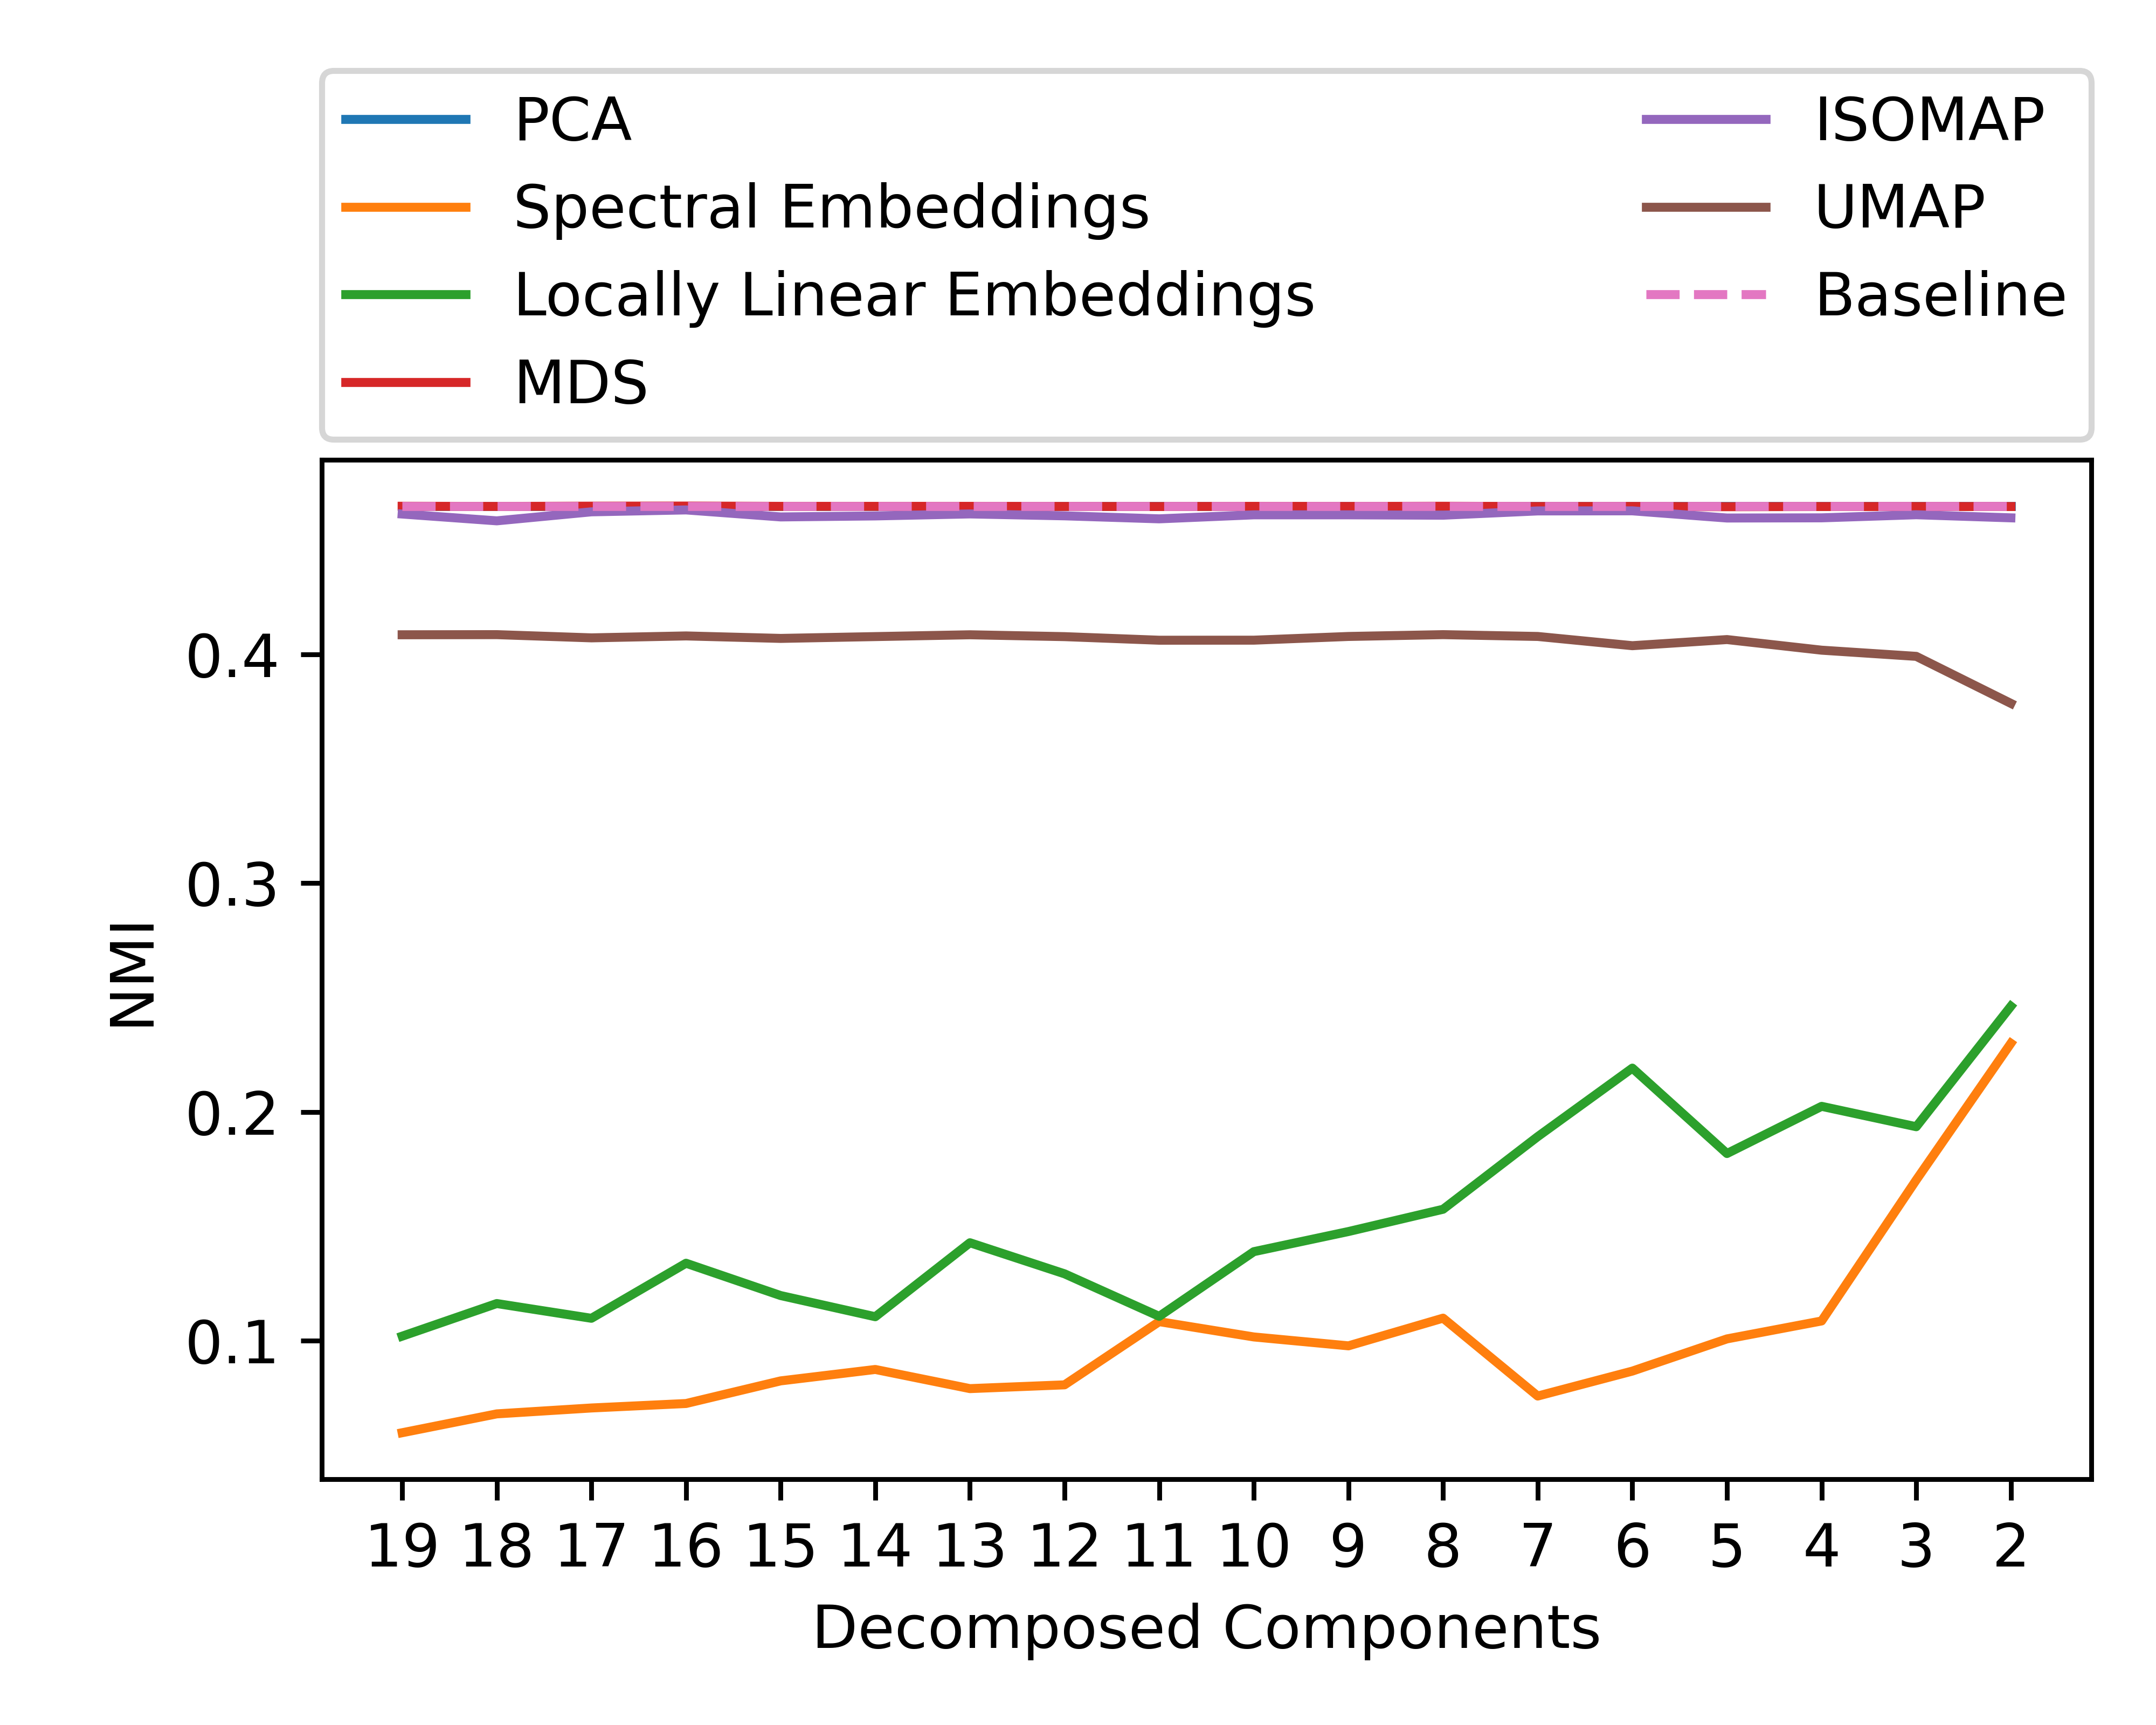
\includegraphics[width=0.48\linewidth]{images/charts_real/real_data_breast_cancer_nmi.png}
                    \label{subfig:breast_cancer:nmi}
                }
                \subfigure[]{
                    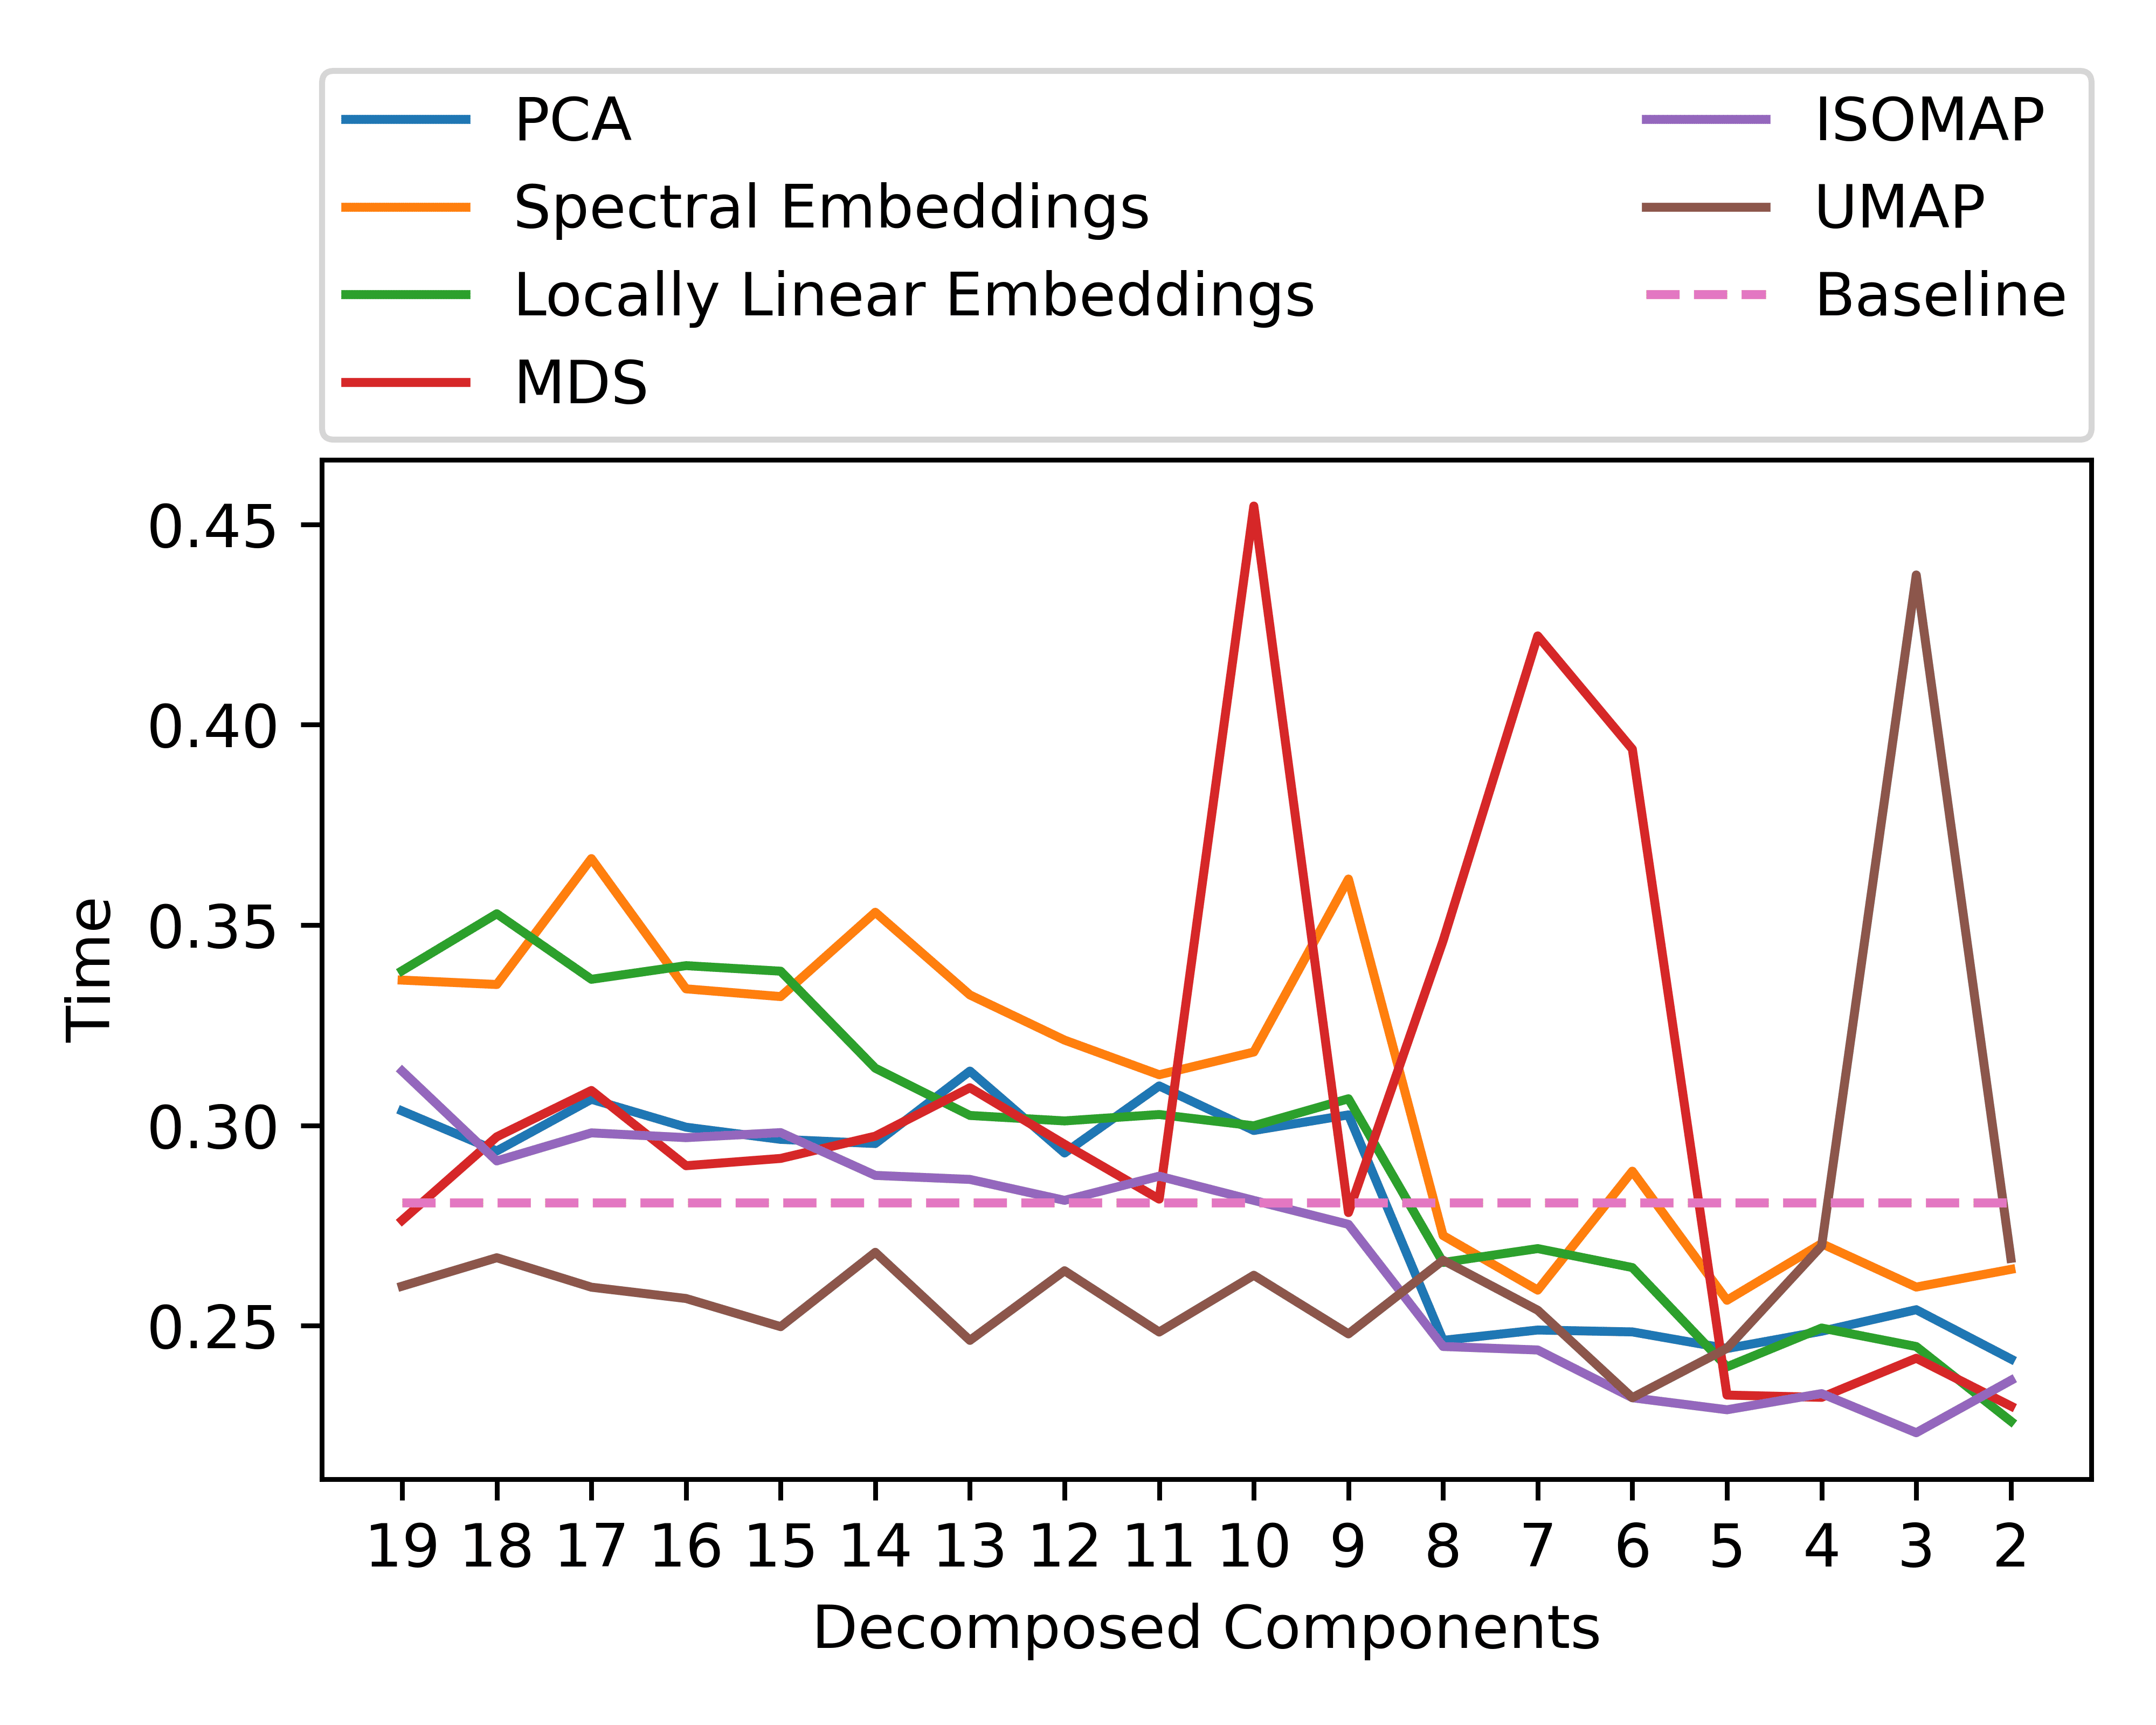
\includegraphics[width=0.48\linewidth]{images/charts_real/real_data_breast_cancer_time.png}
                    \label{subfig:breast_cancer:time}
                }
                \caption{Анализ влияния различных методов снижения размерности данных на кластеризацию набора данных Breast Cancer. Линия Baseline -- результат работы алгоритма \kmeans{} без предварительного снижения размерности. Результаты для
                    \subref{subfig:breast_cancer:ami} AMI;
                    \subref{subfig:breast_cancer:ari} ARI;
                    \subref{subfig:breast_cancer:nmi} NMI, а также на время работы алгоритма \subref{subfig:breast_cancer:time}.
                }
                \label{fig:breast_cancer}
            \end{figure}

            \begin{figure}[H]\centering
                \includegraphics[width=0.99\linewidth]{images/decomposer/breast_cancer_decomposer_analysis.png}
                \caption{Визуализация набора данных Breast Cancer после снижения размерности до 2 с использованием PCA, Spectral Embeddings, Locally Linear Embeddings, MDS, ISOMAP, UMAP.}
                \label{fig:breast_cancer:example}
            \end{figure}

            На рисунке \ref{fig:breast_cancer} представлены результаты применения различных методов снижения размерности перед кластеризацией K-Means на наборе данных Breast Cancer. Наиболее заметную положительную динамику продемонстрировали методы Locally Linear Embeddings (LLE) и Spectral Embeddings -- при уменьшении размерности до 10 и ниже наблюдается последовательный рост метрик кластеризации: AMI, ARI и NMI. Пиковые значения достигаются в точке, где число компонент совпадает с числом кластеров в выборке, что может свидетельствовать о более точной структурной декомпозиции, когда размерность пространства отражает истинное количество скрытых групп. В то же время алгоритмы PCA и MDS демонстрируют стабильные показатели качества, близкие к базовому сценарию кластеризации без предварительного снижения размерности. Это указывает на то, что оба метода хорошо сохраняют глобальную структуру данных, которая является ключевой для работы алгоритма K-Means. Особенно стоит отметить MDS, который обеспечивает не только стабильность качества, но и высокую воспроизводимость результатов на всем диапазоне размерностей. Такое поведение подтверждает различия в подходах: методы LLE и Spectral Embeddings склонны акцентировать внимание на локальных взаимосвязях между точками, что делает их полезными при сильной редукции, в то время как PCA и MDS сохраняют глобальную топологию, важную для более устойчивой кластеризации.

        \subsubsection{Результаты алгоритма на наборе данных Digits}
            Digits -- это стандартный набор данных для многоклассовой классификации, часто используемый в задачах распознавания образов. Данные представляют собой рукописные цифры от 0 до 9, оцифрованные в виде изображений 8x8 пикселей. Каждое изображение преобразовано в матрицу чисел, отражающих интенсивность оттенков серого.

            \begin{table}[H]
                \centering
                \caption{Характеристики набора данных Digits.}
                \begin{tabular}{ccc}
                    \toprule
                    Число классов & Число объектов & Размерность пространства \\
                    \midrule
                    10 & 1797 & 64 \\
                    \bottomrule
                \end{tabular}
            \end{table}

            Набор данных Digits представляет собой матрицу размерностью 1797x64, где каждая строка соответствует одному изображению цифры, а каждый столбец содержит значение яркости пикселя (от 0 до 16). Исходные изображения были нормализованы для уменьшения влияния вариаций наклона и толщины линий.

            \begin{figure}[H]\centering
                \subfigure[]{
                    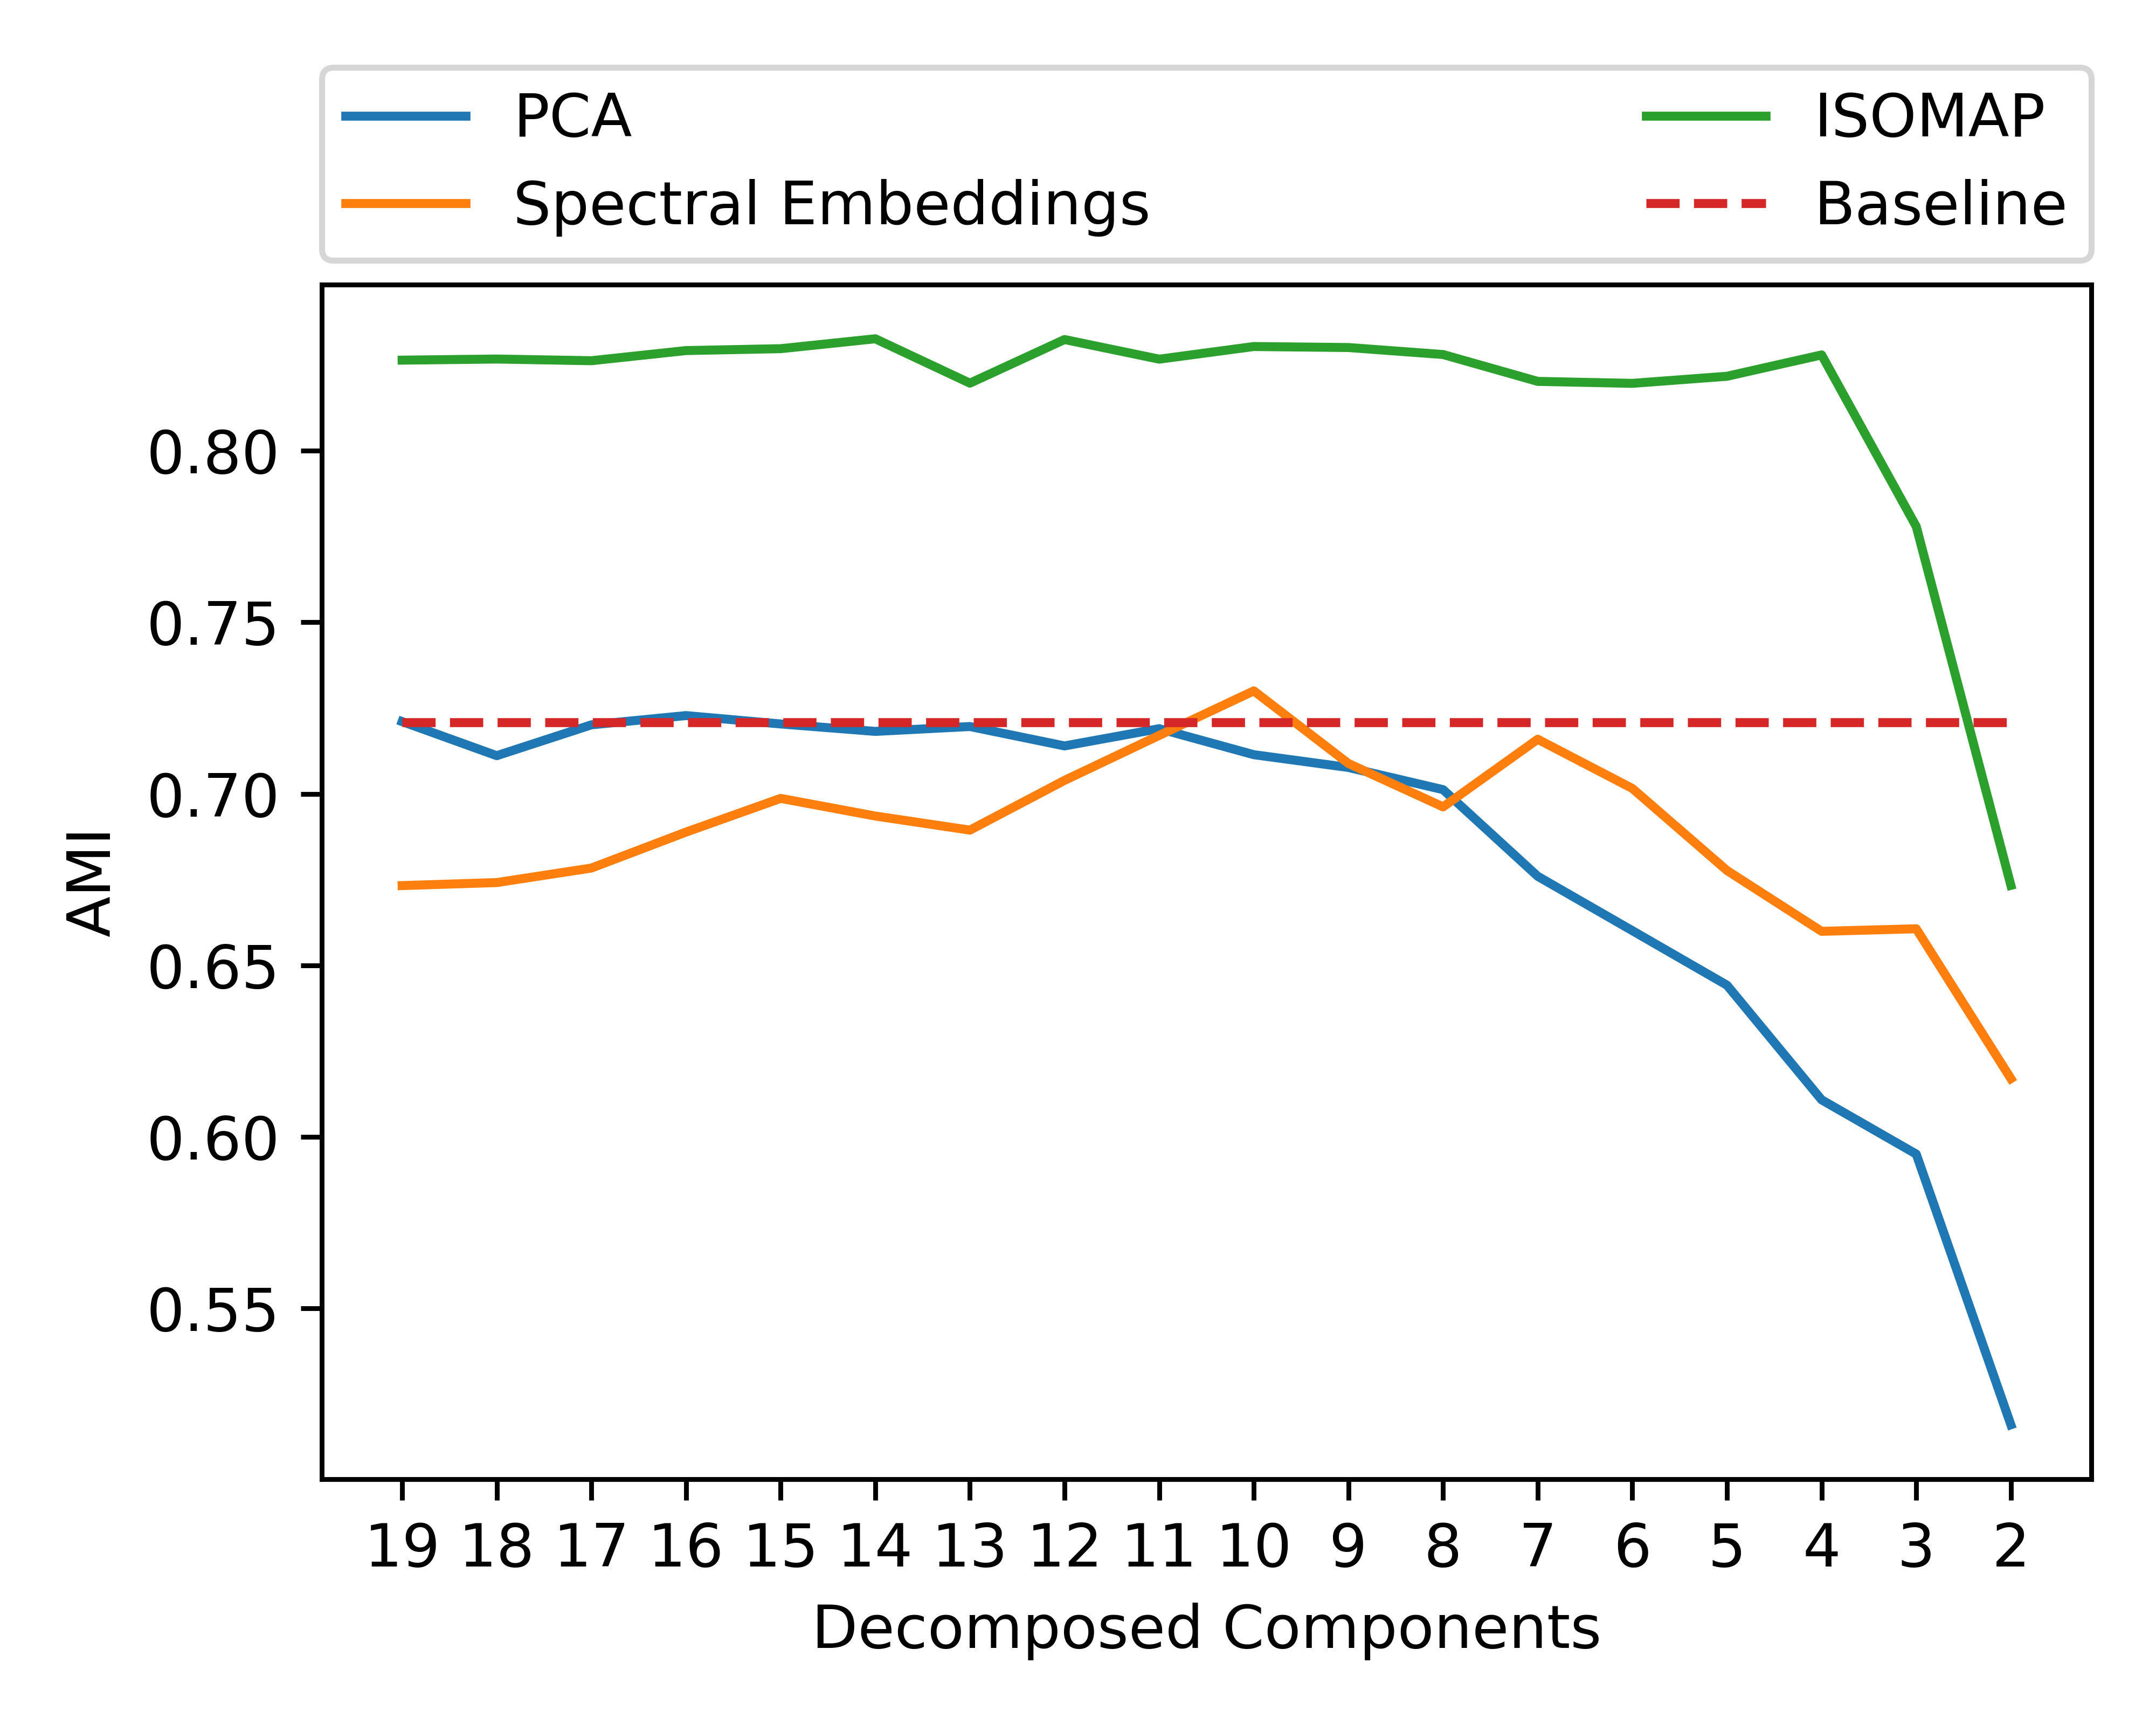
\includegraphics[width=0.48\linewidth]{images/charts_real/real_data_digits_ami.png}
                    \label{subfig:digits:ami}
                }
                \subfigure[]{
                    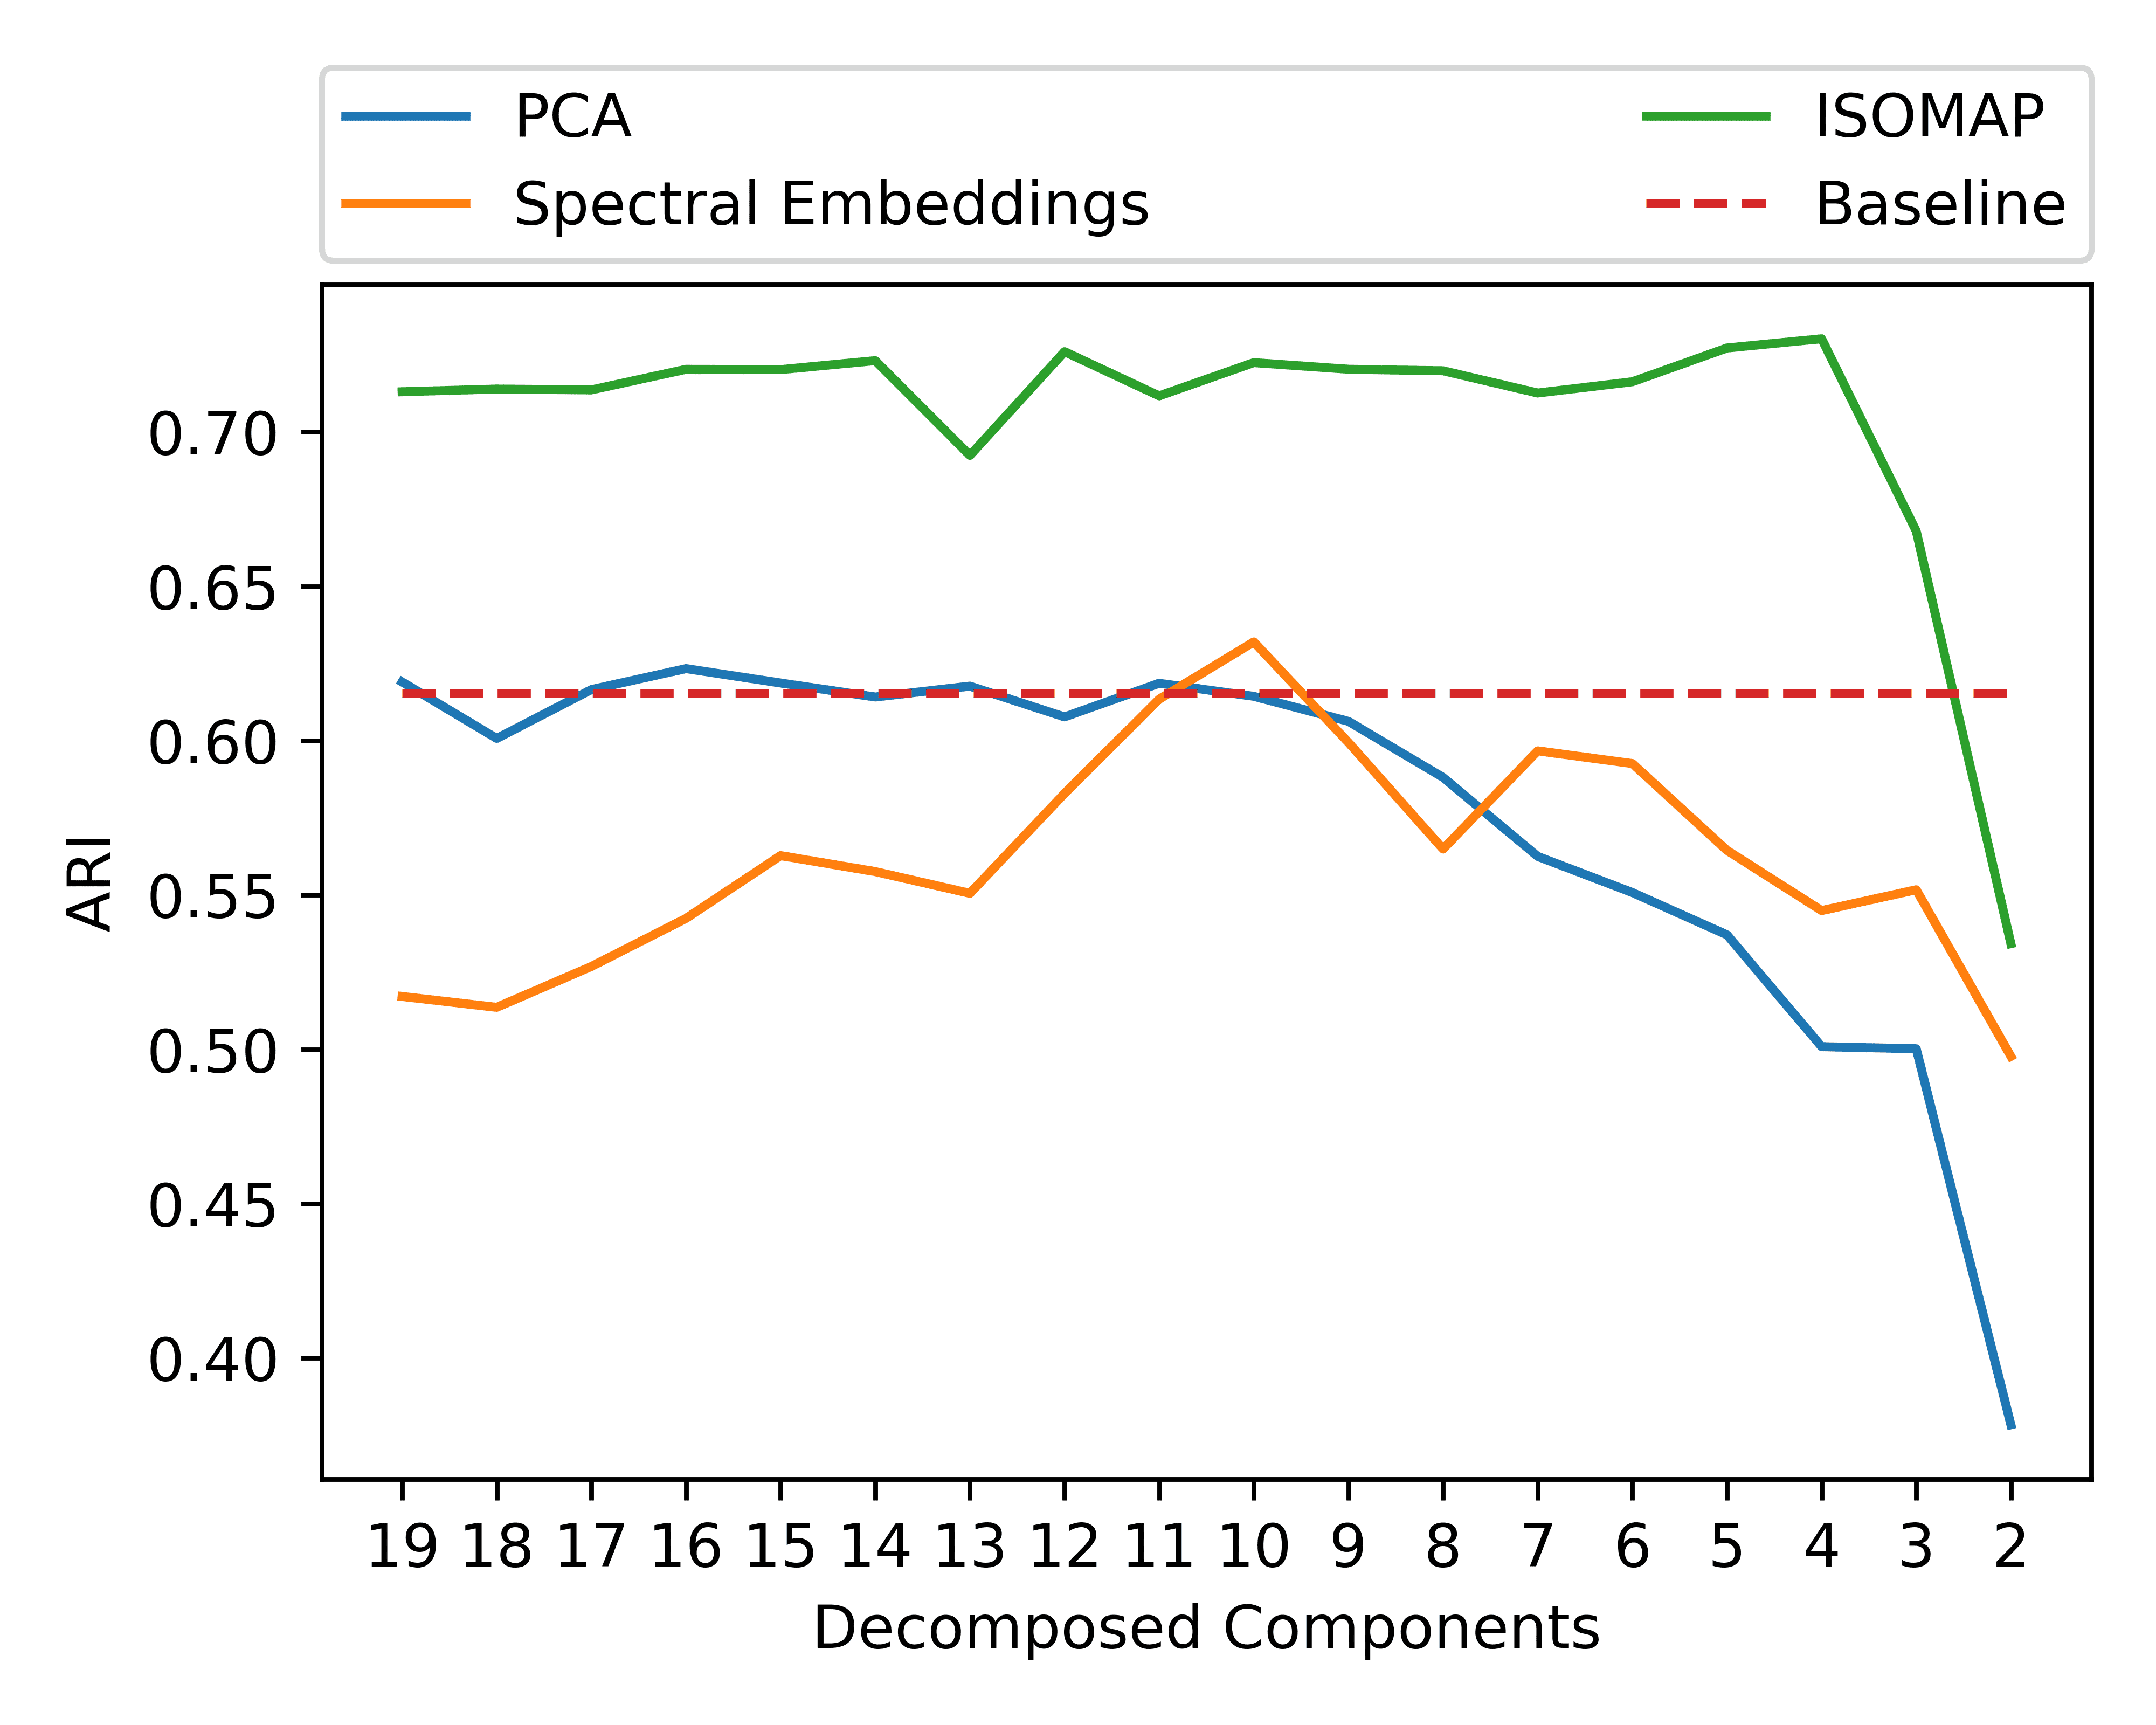
\includegraphics[width=0.48\linewidth]{images/charts_real/real_data_digits_ari.png}
                    \label{subfig:digits:ari}
                }
                \subfigure[]{
                    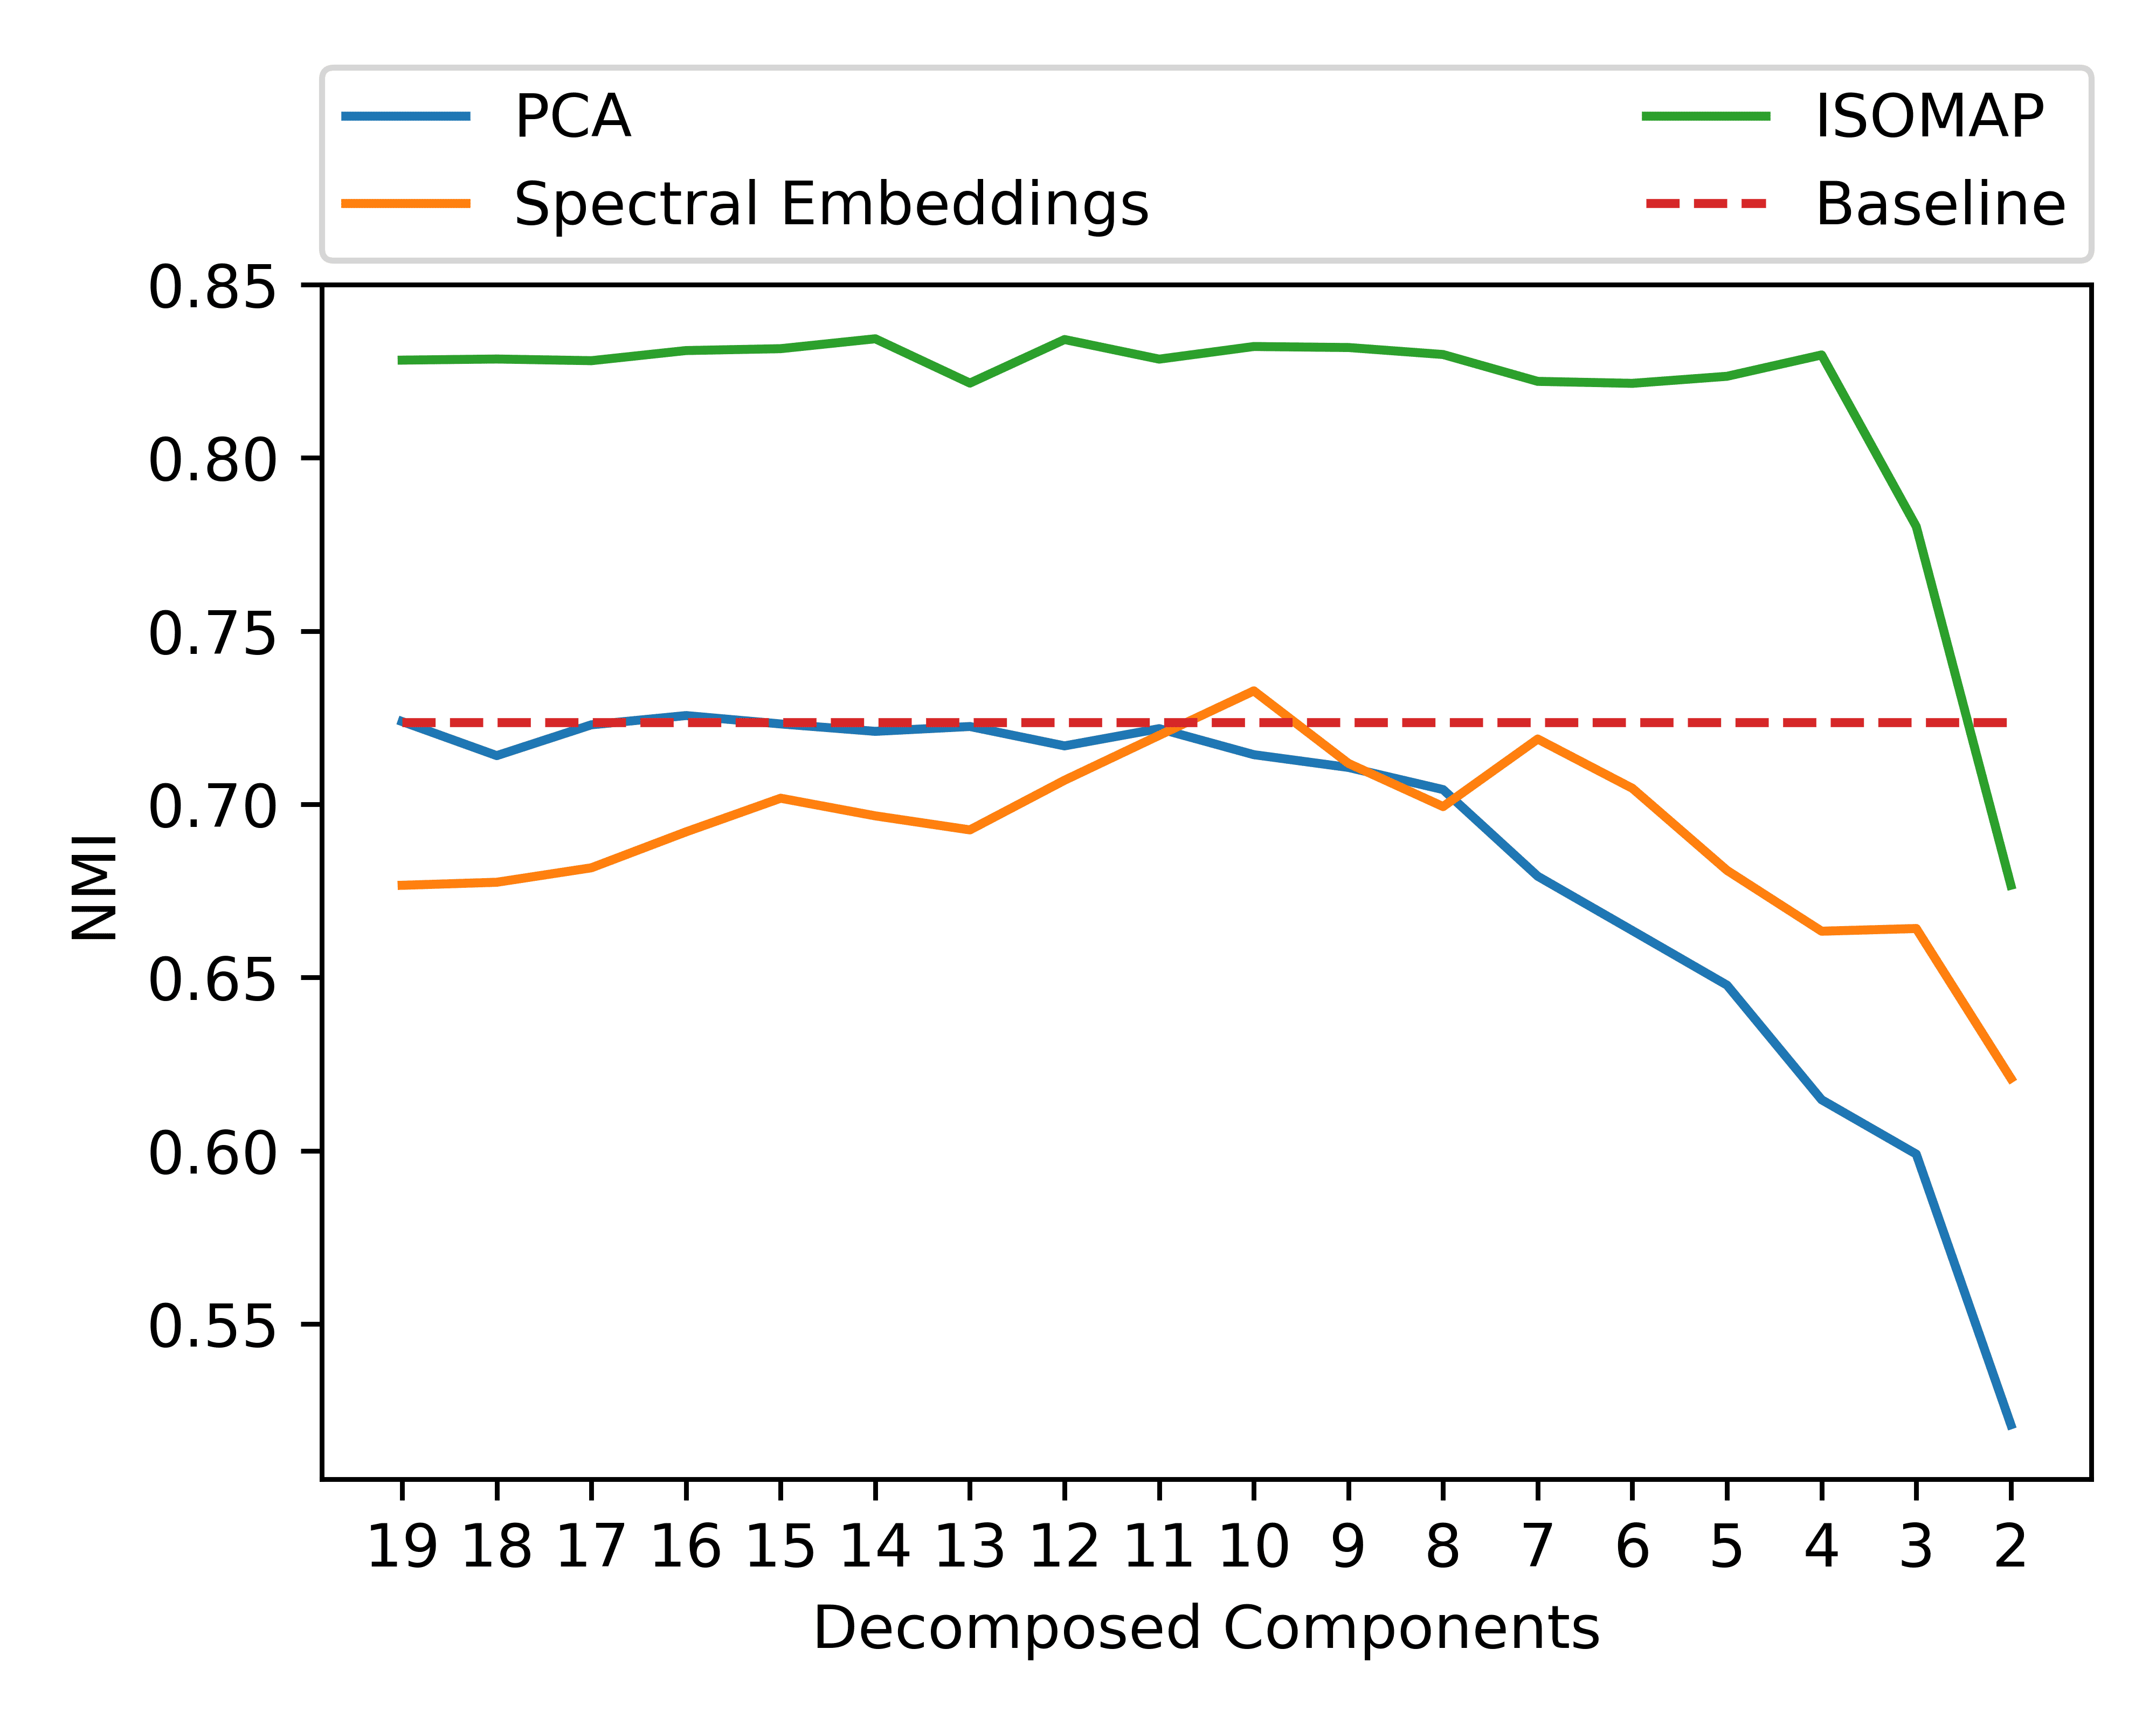
\includegraphics[width=0.48\linewidth]{images/charts_real/real_data_digits_nmi.png}
                    \label{subfig:digits:nmi}
                }
                \subfigure[]{
                    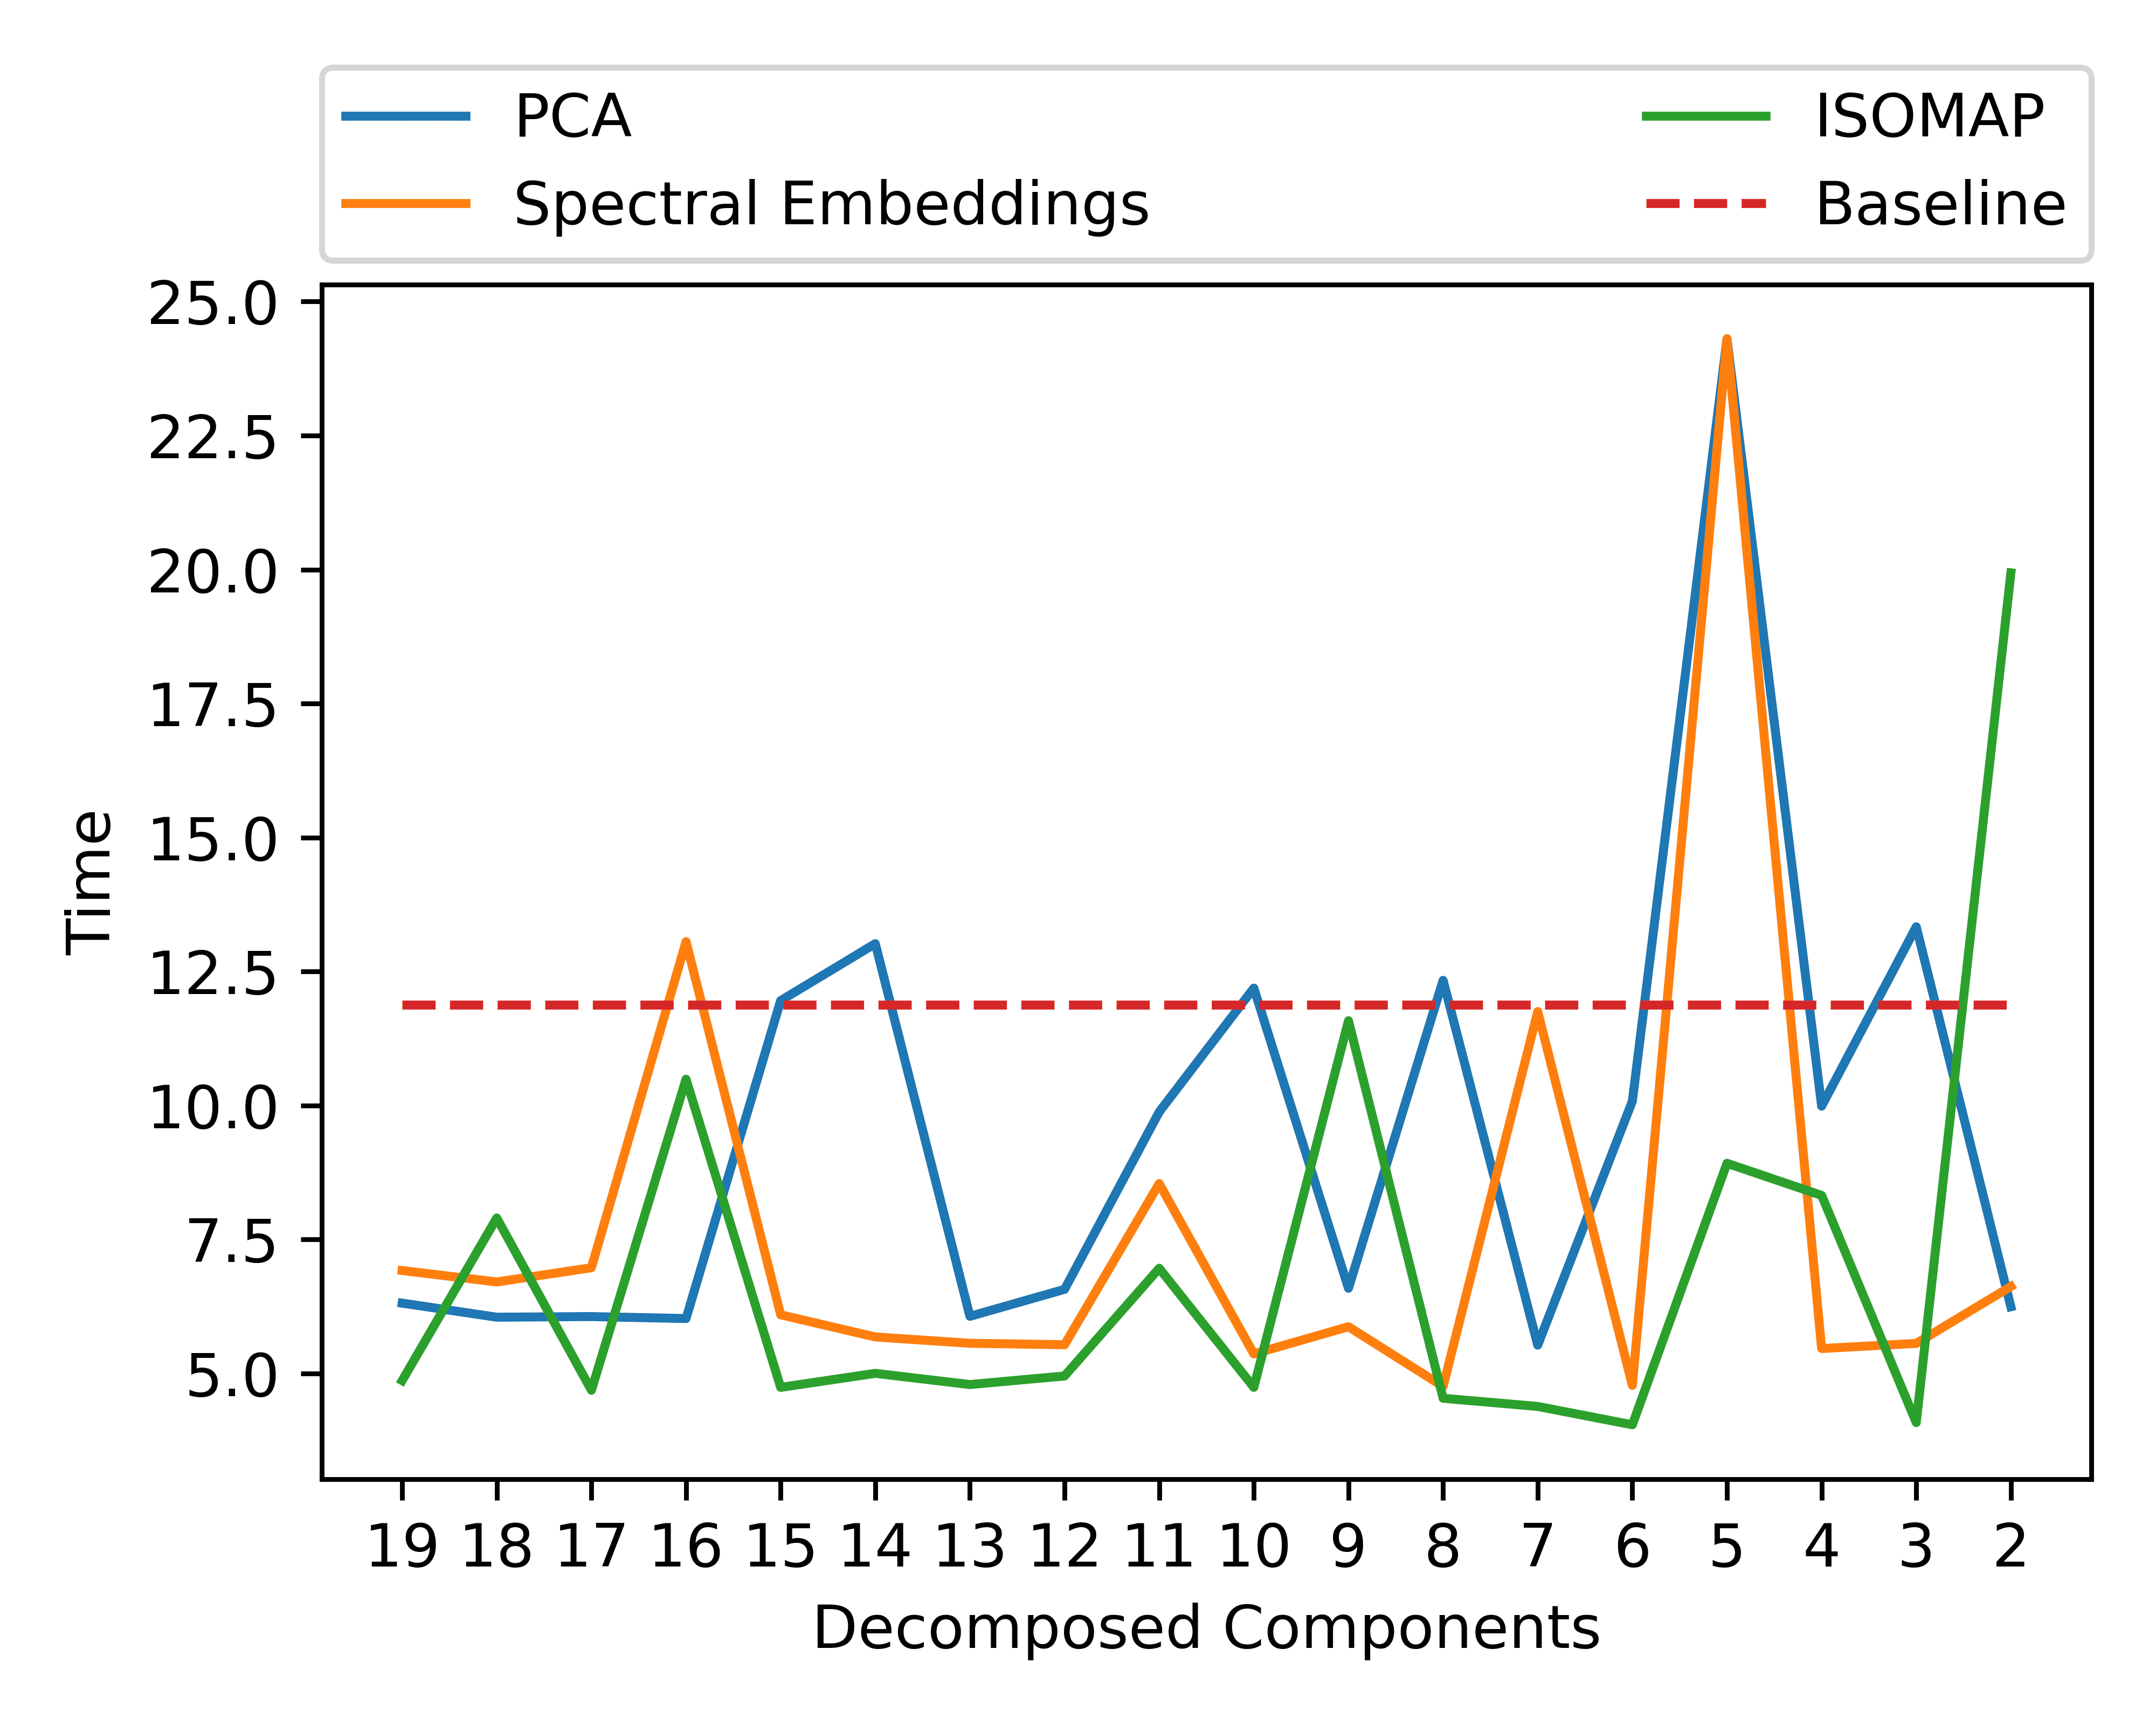
\includegraphics[width=0.48\linewidth]{images/charts_real/real_data_digits_time.png}
                    \label{subfig:digits:time}
                }
                \caption{Анализ влияния различных методов снижения размерности данных на кластеризацию набора данных Digits. Линия Baseline -- результат работы алгоритма \kmeans{} без предварительного снижения размерности. Результаты для
                    \subref{subfig:digits:ami} AMI;
                    \subref{subfig:digits:ari} ARI;
                    \subref{subfig:digits:nmi} NMI, а также на время работы алгоритма \subref{subfig:digits:time}.
                }
                \label{fig:digits}
            \end{figure}

            \begin{figure}[H]\centering
                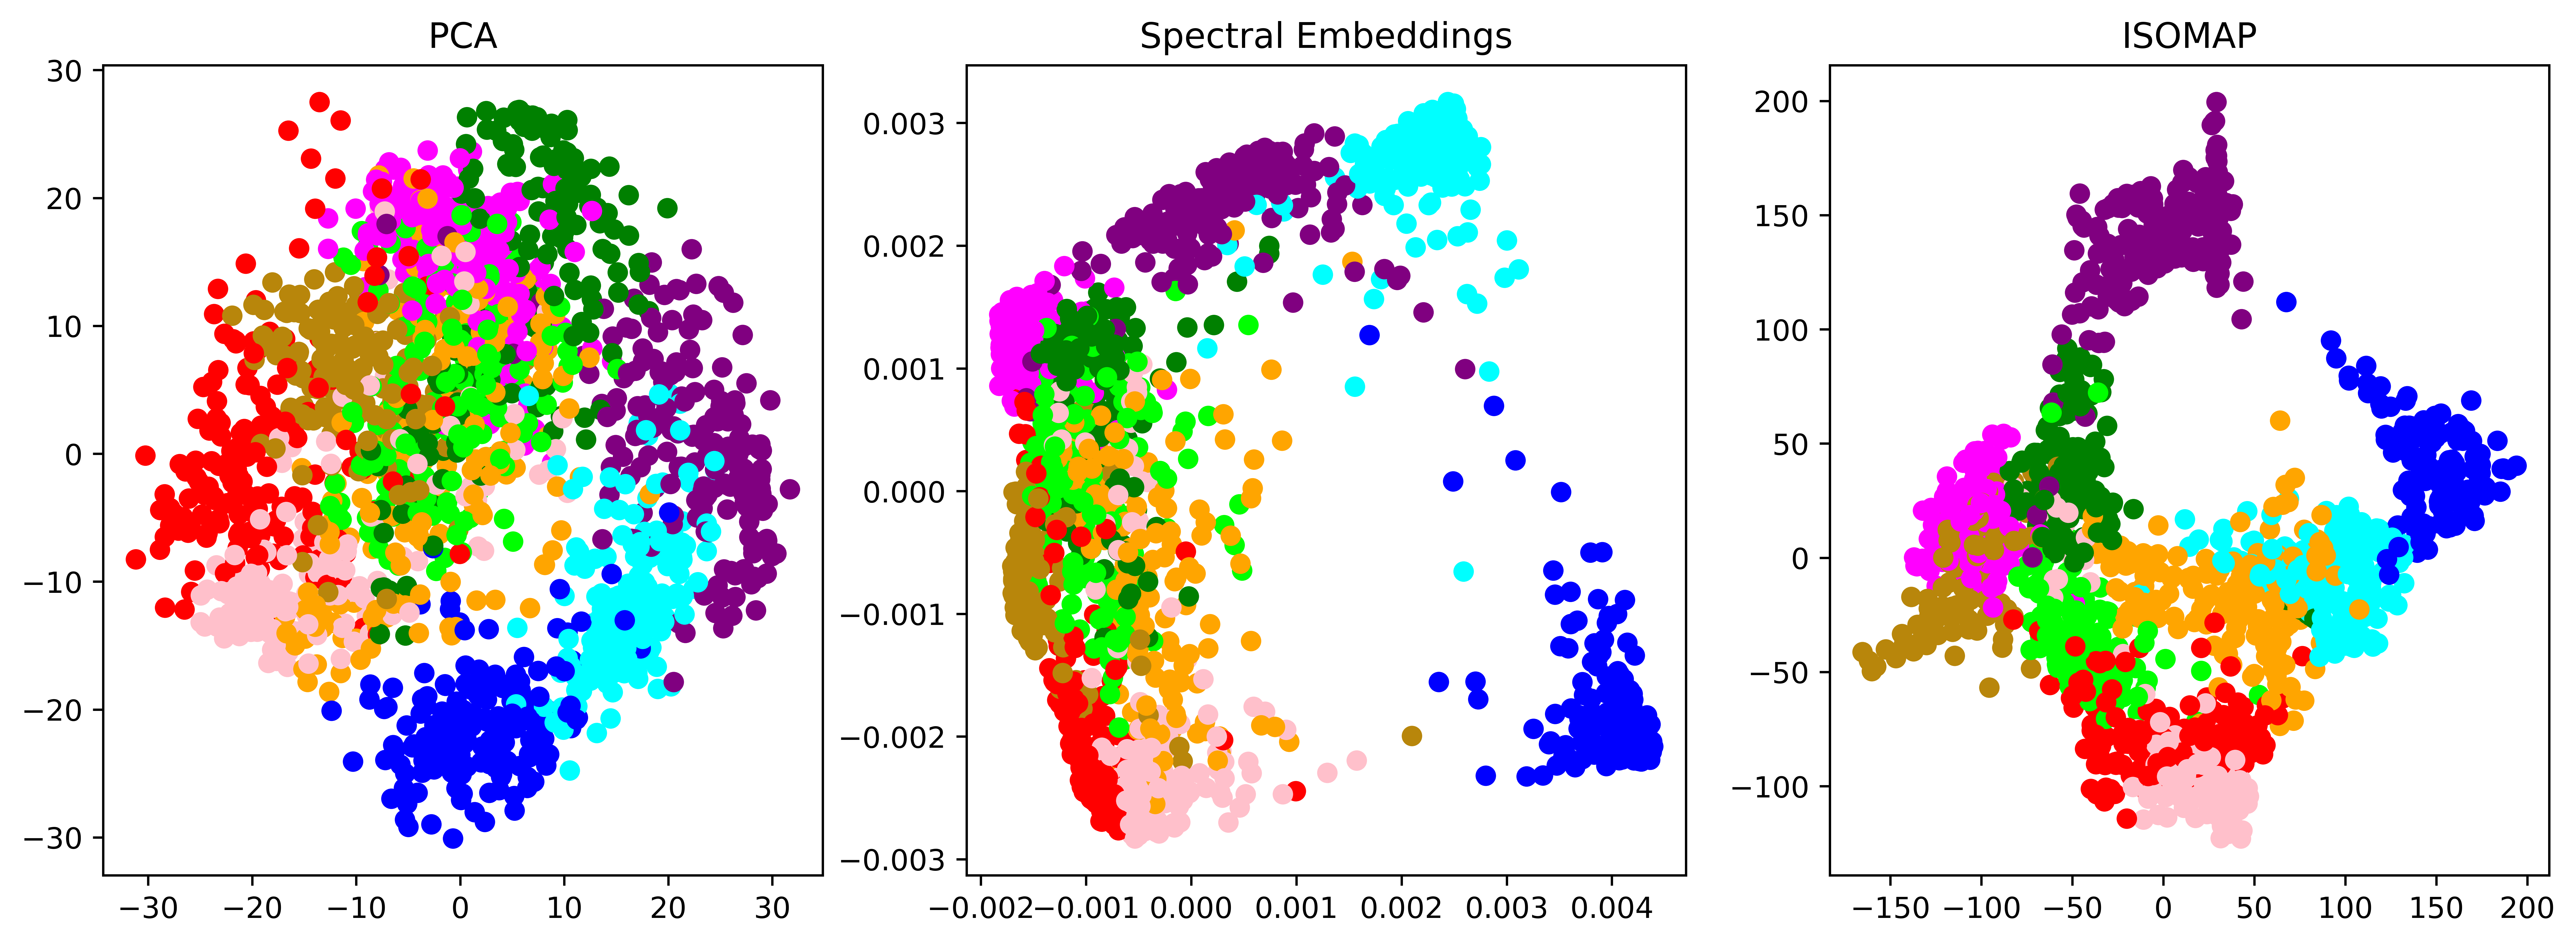
\includegraphics[width=0.99\linewidth]{images/decomposer/digits_decomposer_analysis.png}
                \caption{Визуализация набора данных Digits после снижения размерности до 2 с использованием PCA, Spectral Embeddings, ISOMAP.}
                \label{fig:digits:example}
            \end{figure}

            На рисунке \ref{fig:digits} представлены результаты экспериментов на наборе данных Digits. Следует отметить, что из-за ограничений существующей программной реализации методы Locally Linear Embeddings, MDS и UMAP не смогли корректно выполнить процедуру снижения размерности на этом наборе данных для последующей кластеризации и, таким образом, были исключены из анализа. Среди протестированных алгоритмов ярким лидером оказался ISOMAP, который уверенно превзошел остальные методы по всем основным метрикам кластеризации - AMI, ARI и NMI. Он продемонстрировал стабильное превосходство над базовой линией (результат кластеризации без снижения размерности) вплоть до размерности в 2 компоненты, что говорит о его способности сохранять глобальную геометрию данных даже в сильно сжатом пространстве. Метод PCA продемонстрировал устойчивую деградацию качества кластеризации при уменьшении числа компонент, особенно заметную ниже порога в 10 компонент. Это отражает его ограниченность в улавливании нелинейных зависимостей в данных. Spectral Embedding, напротив, показал результаты в целом ниже уровня базового \kmeans{}, что может объясняться тем, что он оптимизирует локальные отношения между точками, а не глобальную структуру. Тем не менее, на размерности, равной числу кластеров, наблюдался кратковременный всплеск метрик, что, вероятно, связано с тем, что алгоритм эффективно извлекает локальные кластеры, когда размерность достаточно для сохранения этих структур. Также была выявлена интересная зависимость по времени выполнения: ISOMAP, несмотря на свою сложность, в среднем демонстрировал сравнительно низкое время работы с редкими всплесками, что делает его не только точным, но и потенциально пригодным для практического применения при разумной конфигурации.

        \subsubsection{Результаты алгоритма на наборе данных Wine}
            Wine -- это стандартный и простой набор данных для многоклассовой классификации. Эти данные являются результатами химического анализа вин, выращенных в одном и том же регионе Италии тремя разными производителями. Существует тринадцать различных измерений, проведенных для различных компонентов, содержащихся в трех сортах вина.

            \begin{table}[H]
                \centering
                \caption{Характеристики набора данных Wine.}
                \begin{tabular}{ccc}
                    \toprule
                    Число классов &   Число объектов &   Размерность пространства \\
                    \midrule
                    3    &  178 &  13 \\
                    \bottomrule
                \end{tabular}
            \end{table}

            Набор данных Wine представляет собой матрицу с размерностью 178x13, где каждая строка соответствует отдельному образцу вина, а каждый столбец содержит значение конкретного химического измерения.

            \begin{figure}[H]\centering
                \subfigure[]{
                    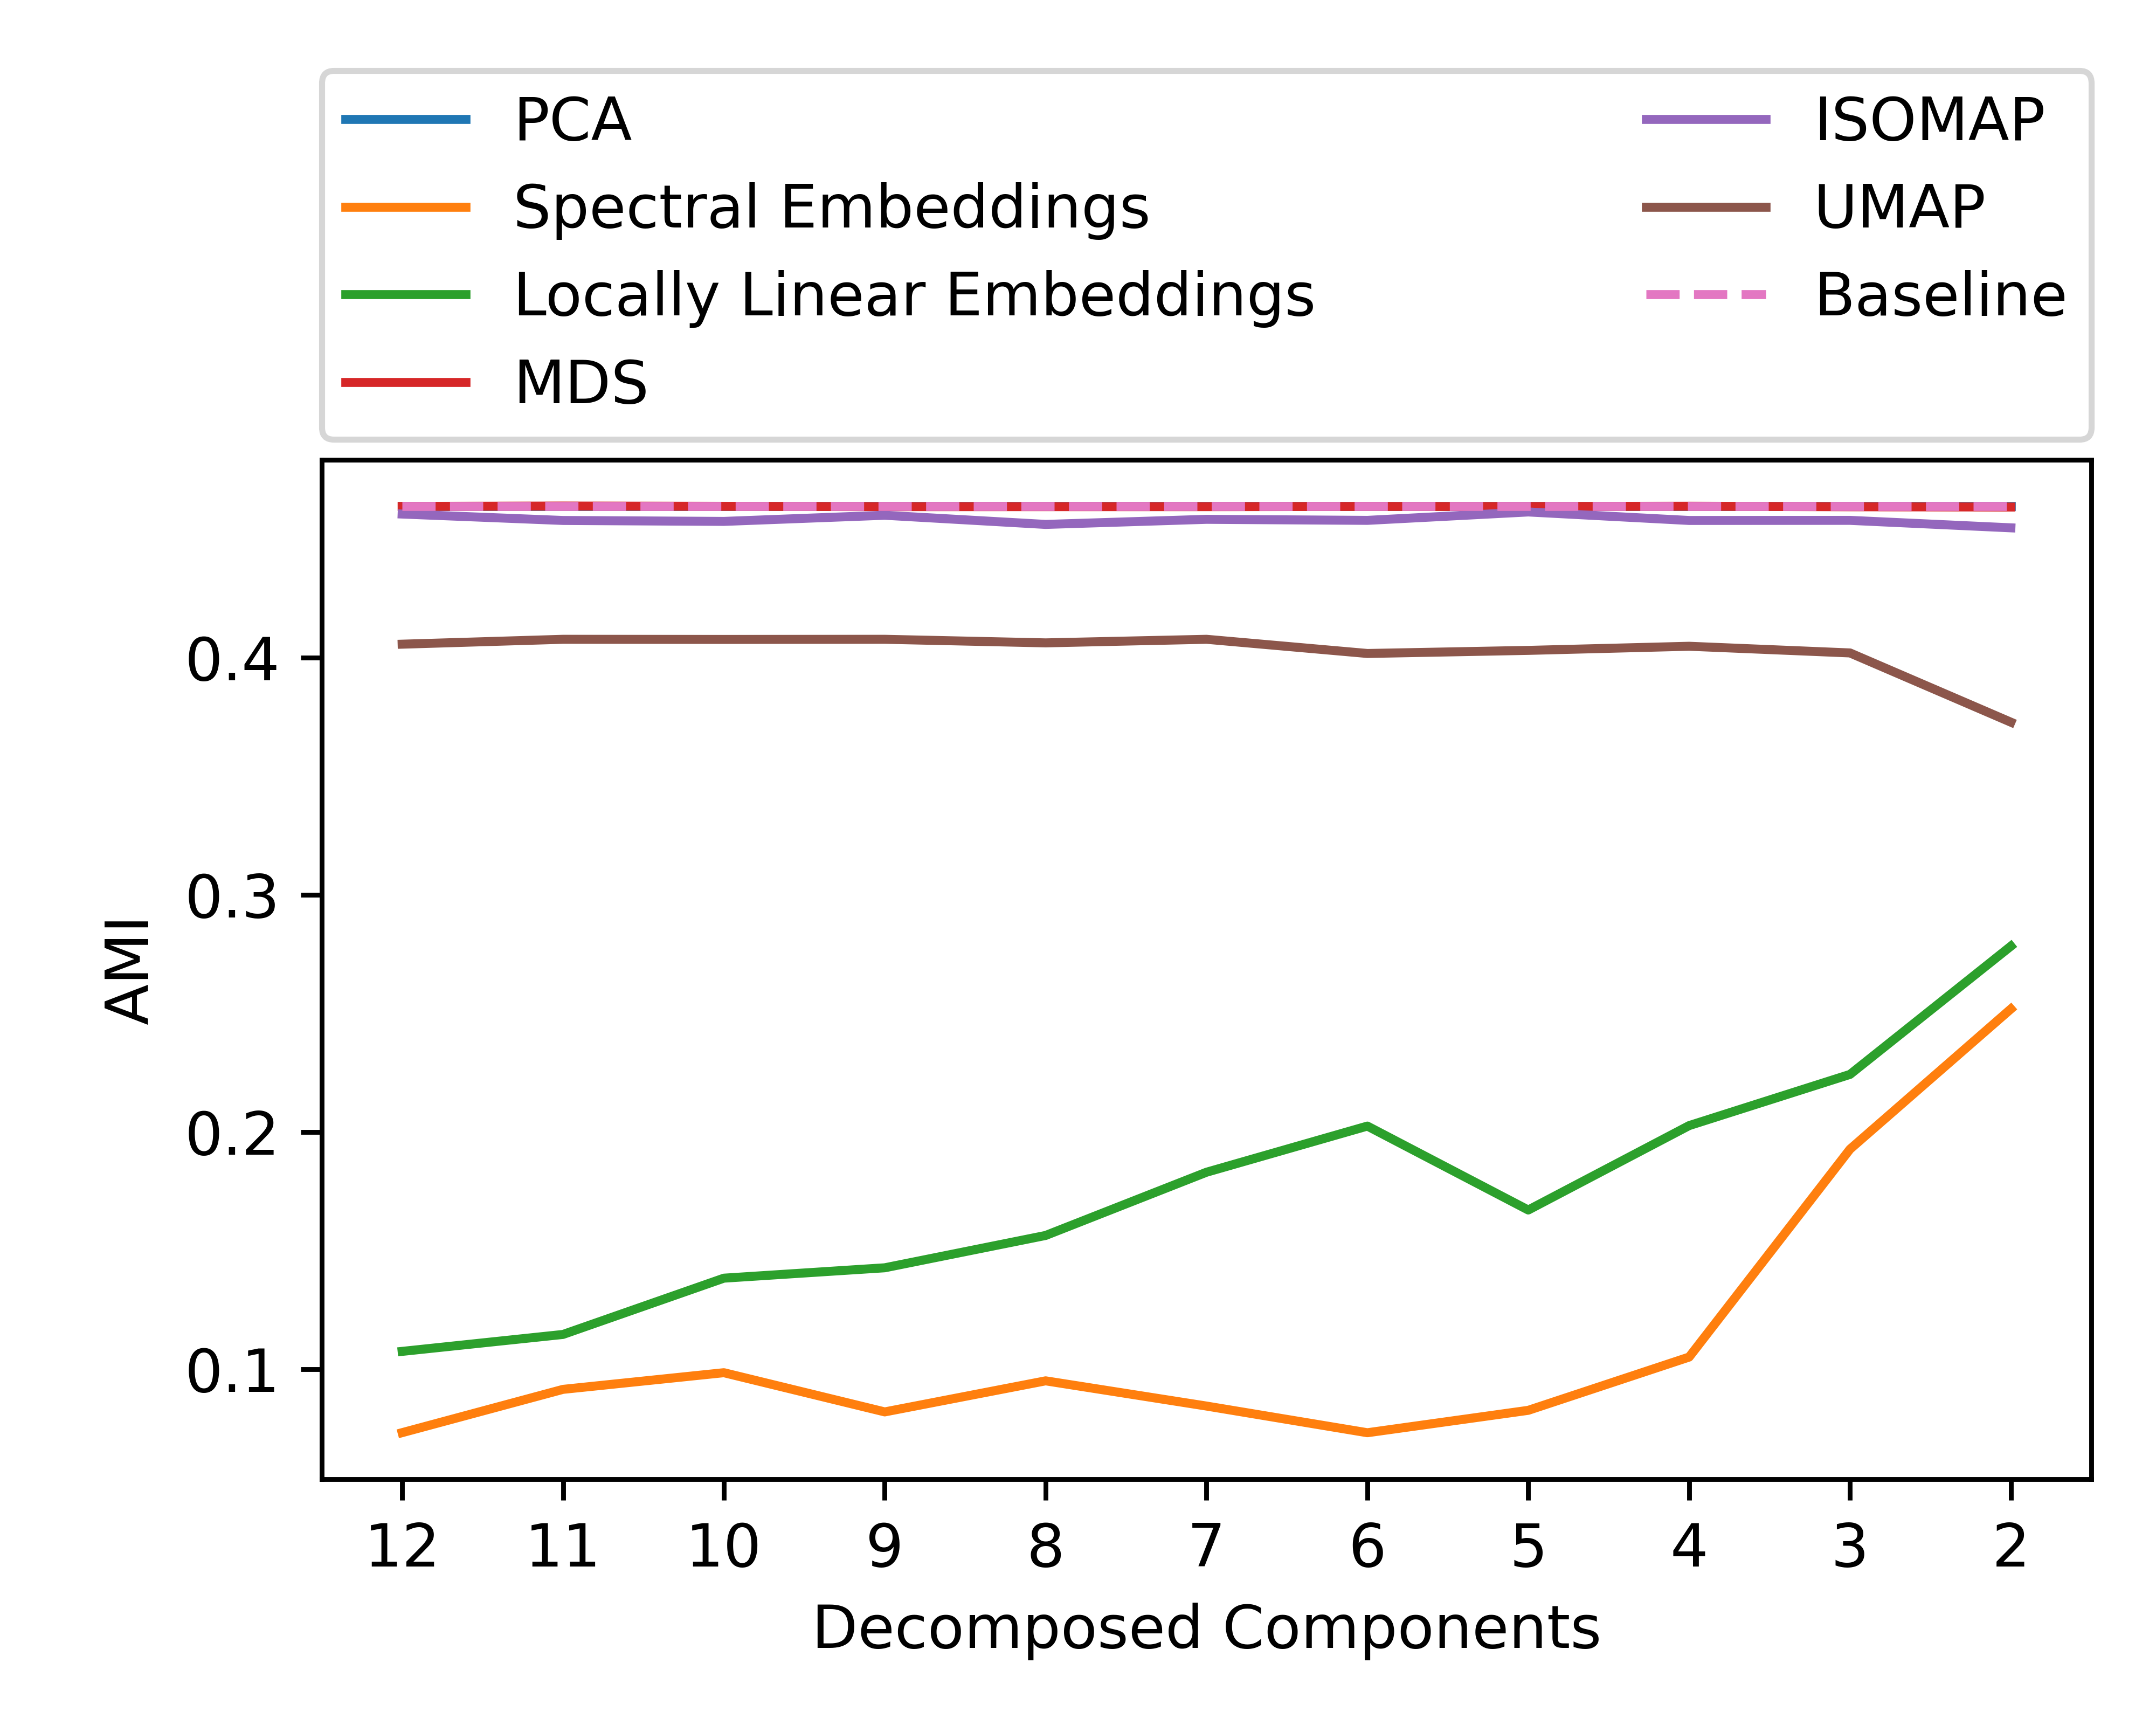
\includegraphics[width=0.48\linewidth]{images/charts_real/real_data_wine_ami.png}
                    \label{subfig:wine:ami}
                }
                \subfigure[]{
                    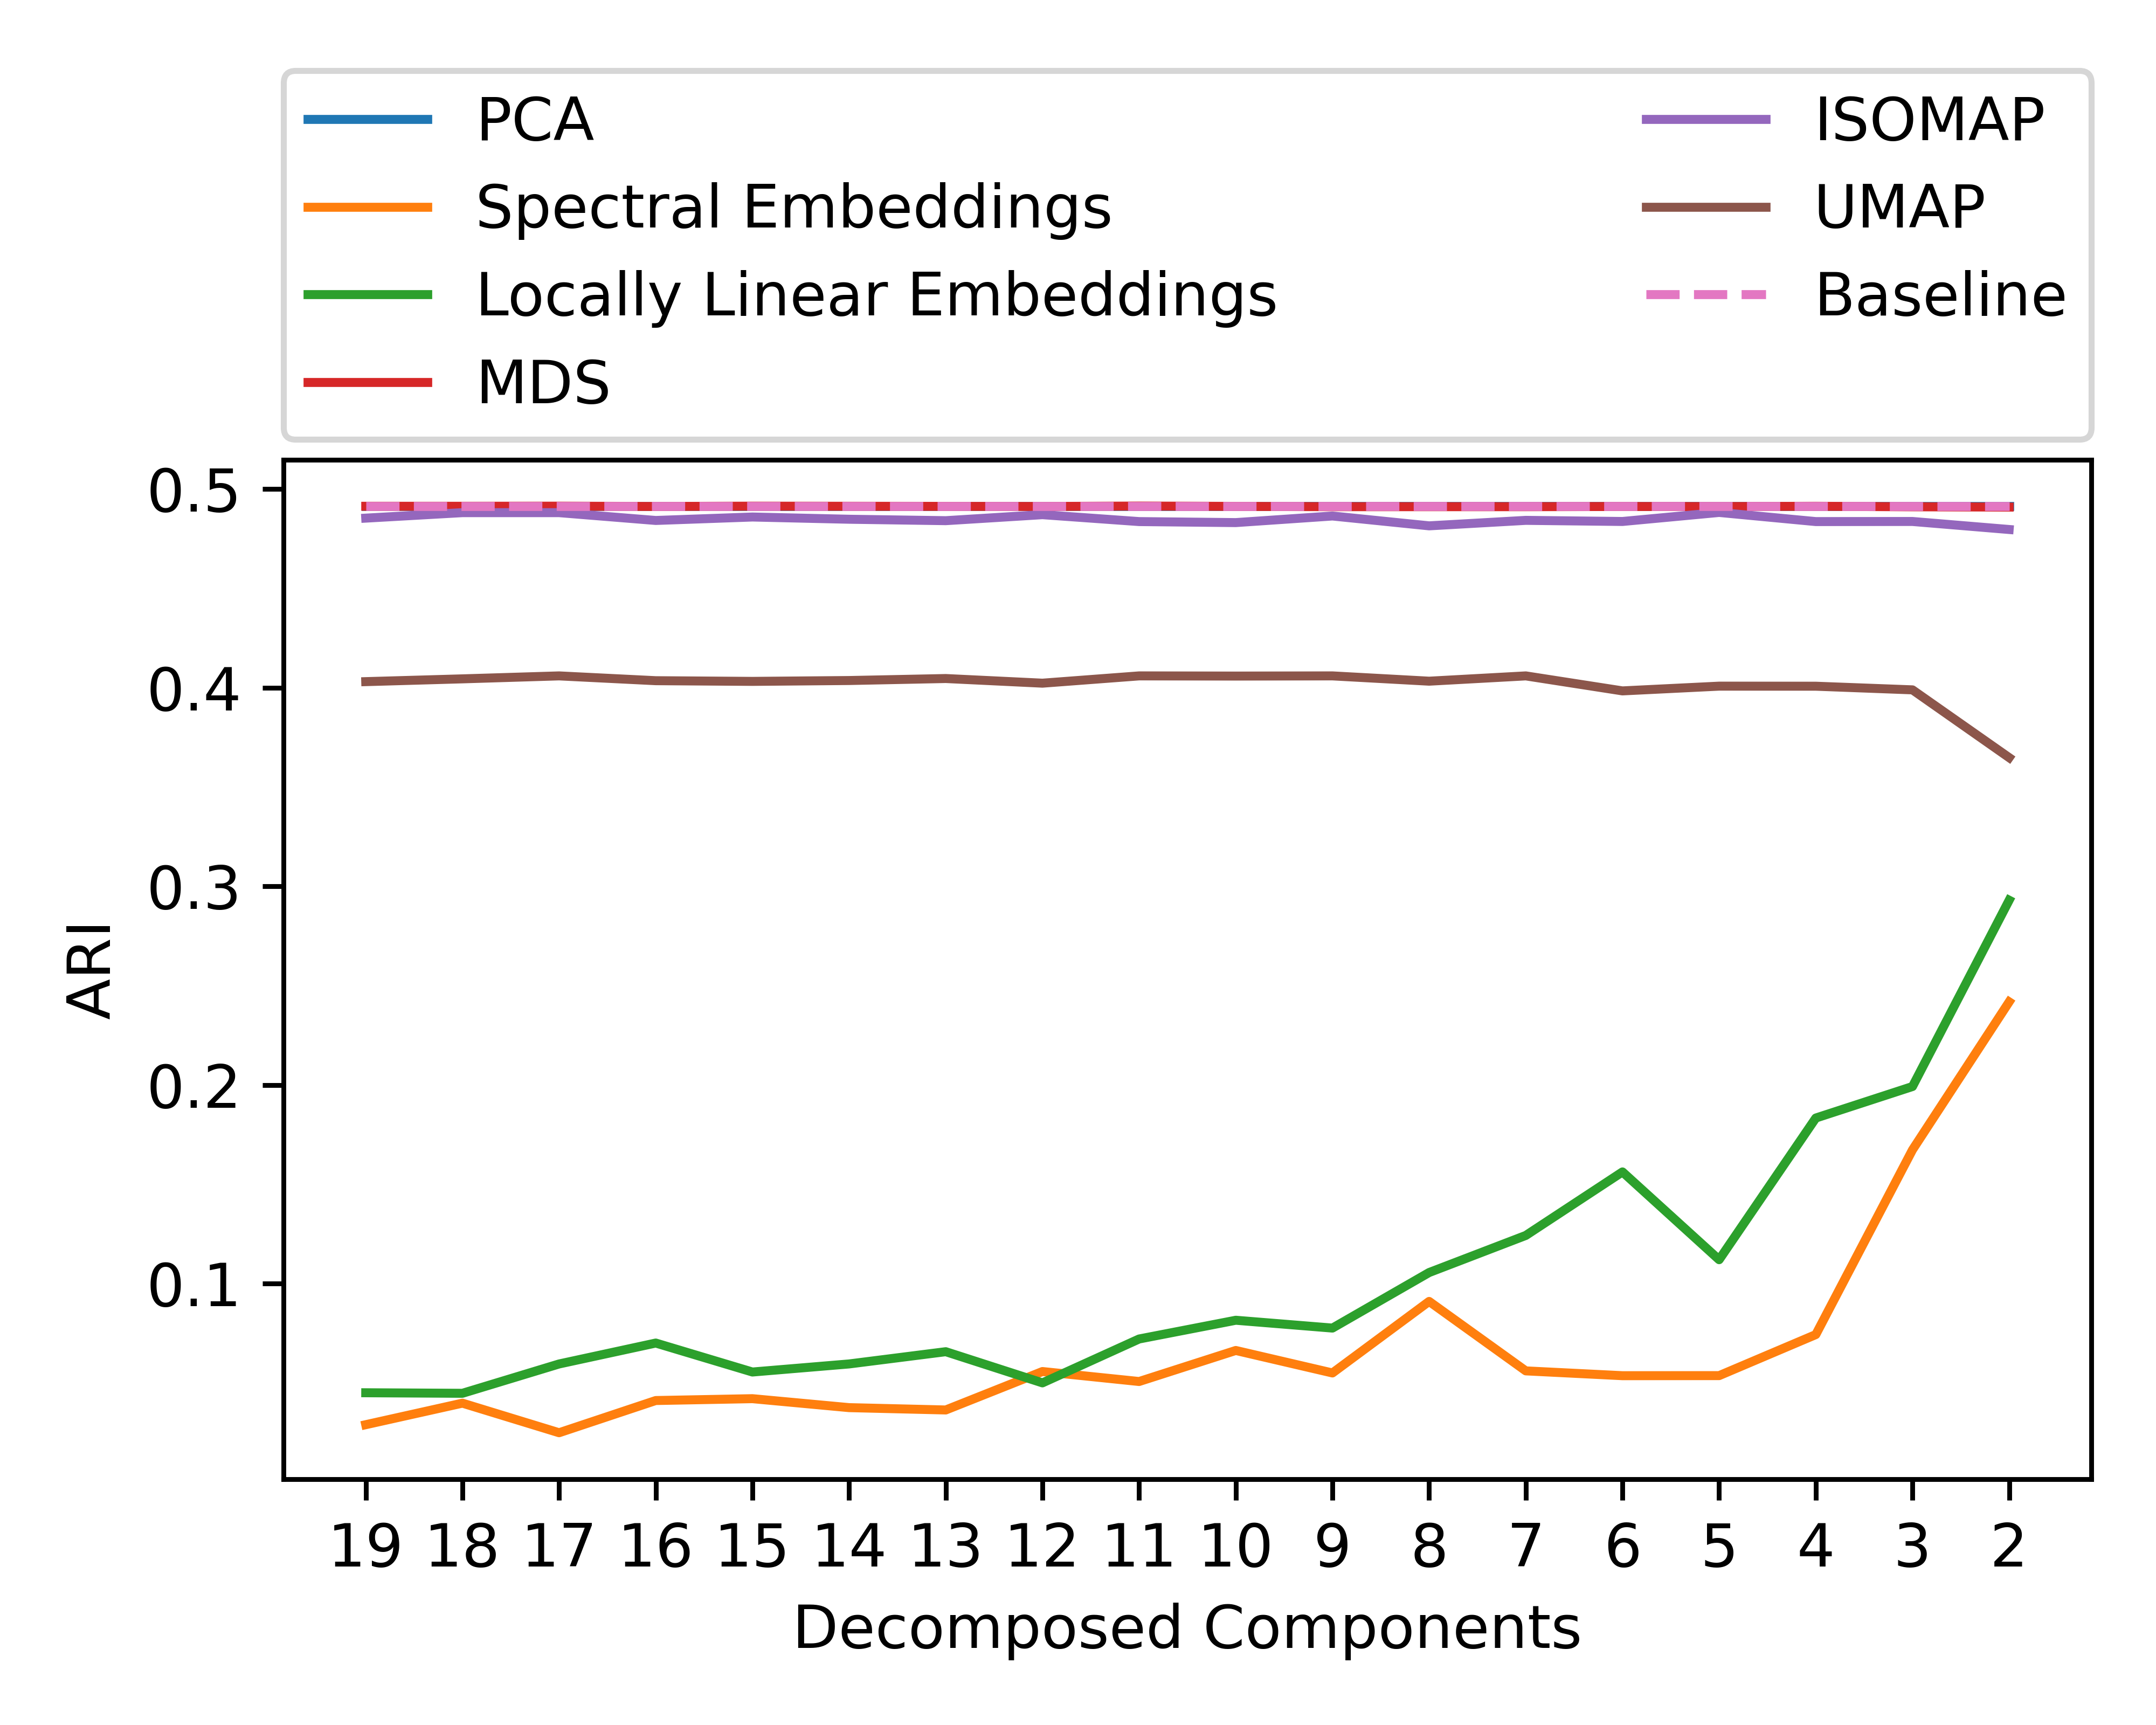
\includegraphics[width=0.48\linewidth]{images/charts_real/real_data_wine_ari.png}
                    \label{subfig:wine:ari}
                }
                \subfigure[]{
                    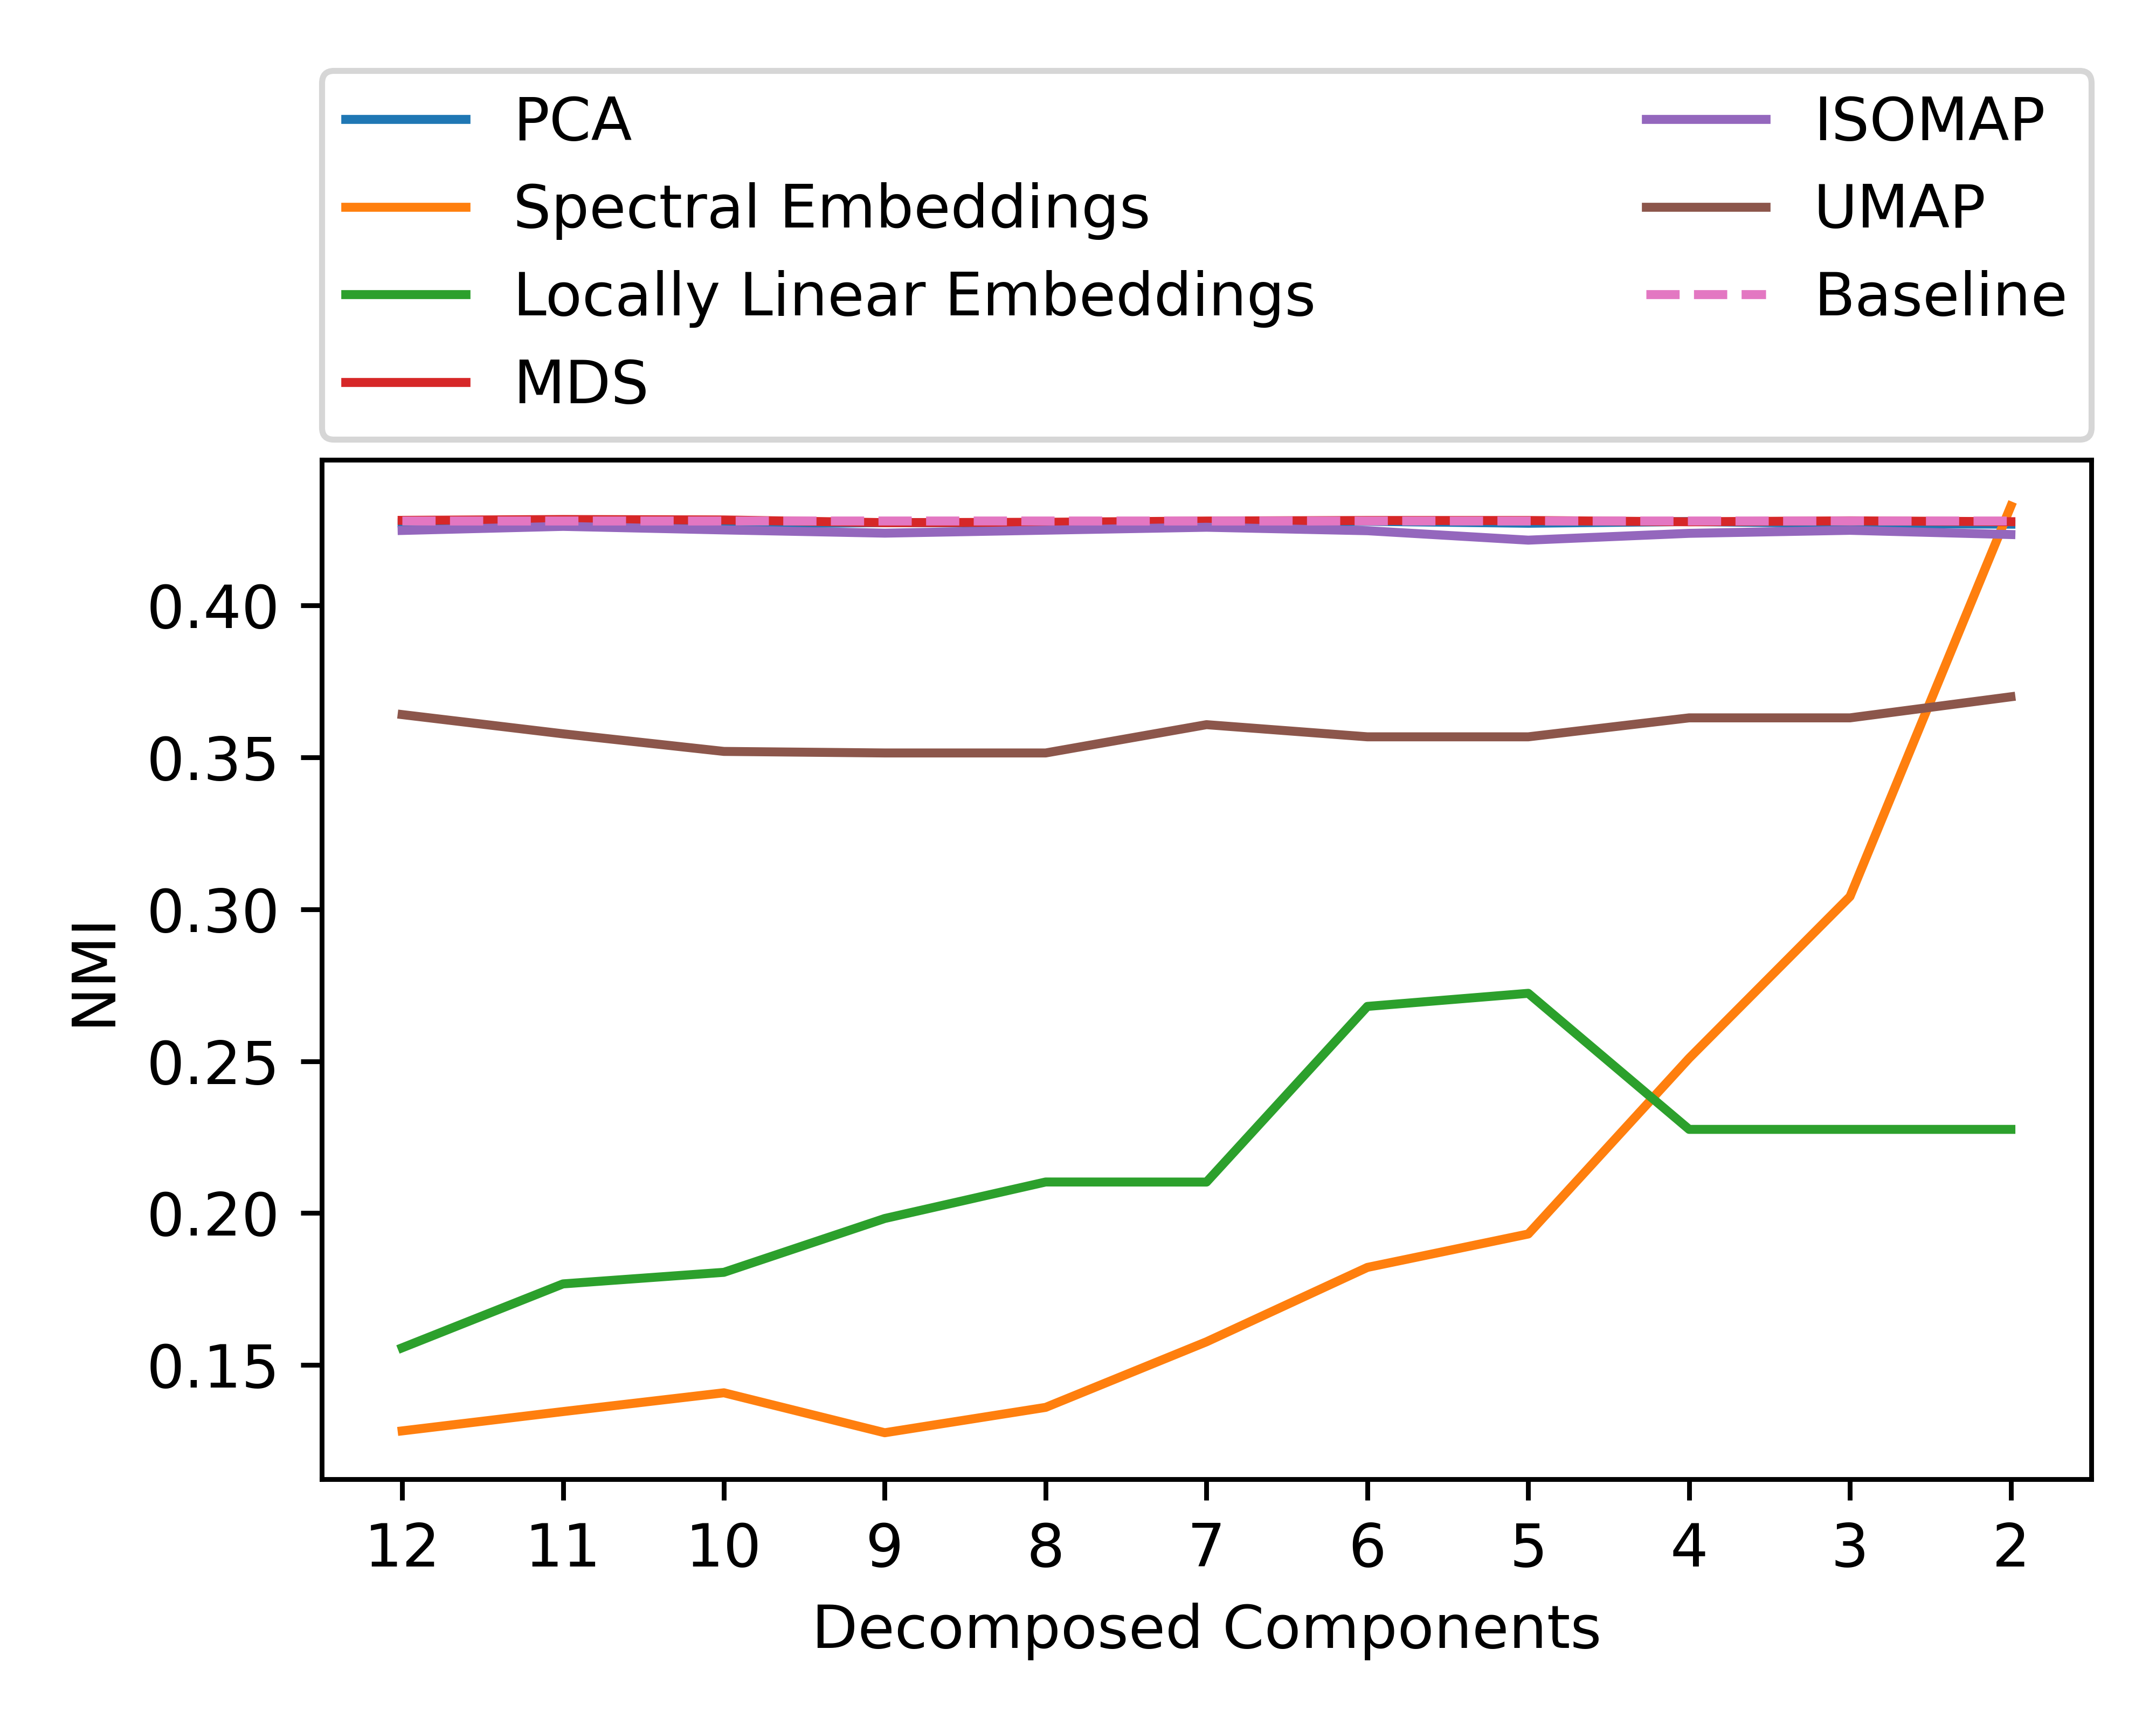
\includegraphics[width=0.48\linewidth]{images/charts_real/real_data_wine_nmi.png}
                    \label{subfig:wine:nmi}
                }
                \subfigure[]{
                    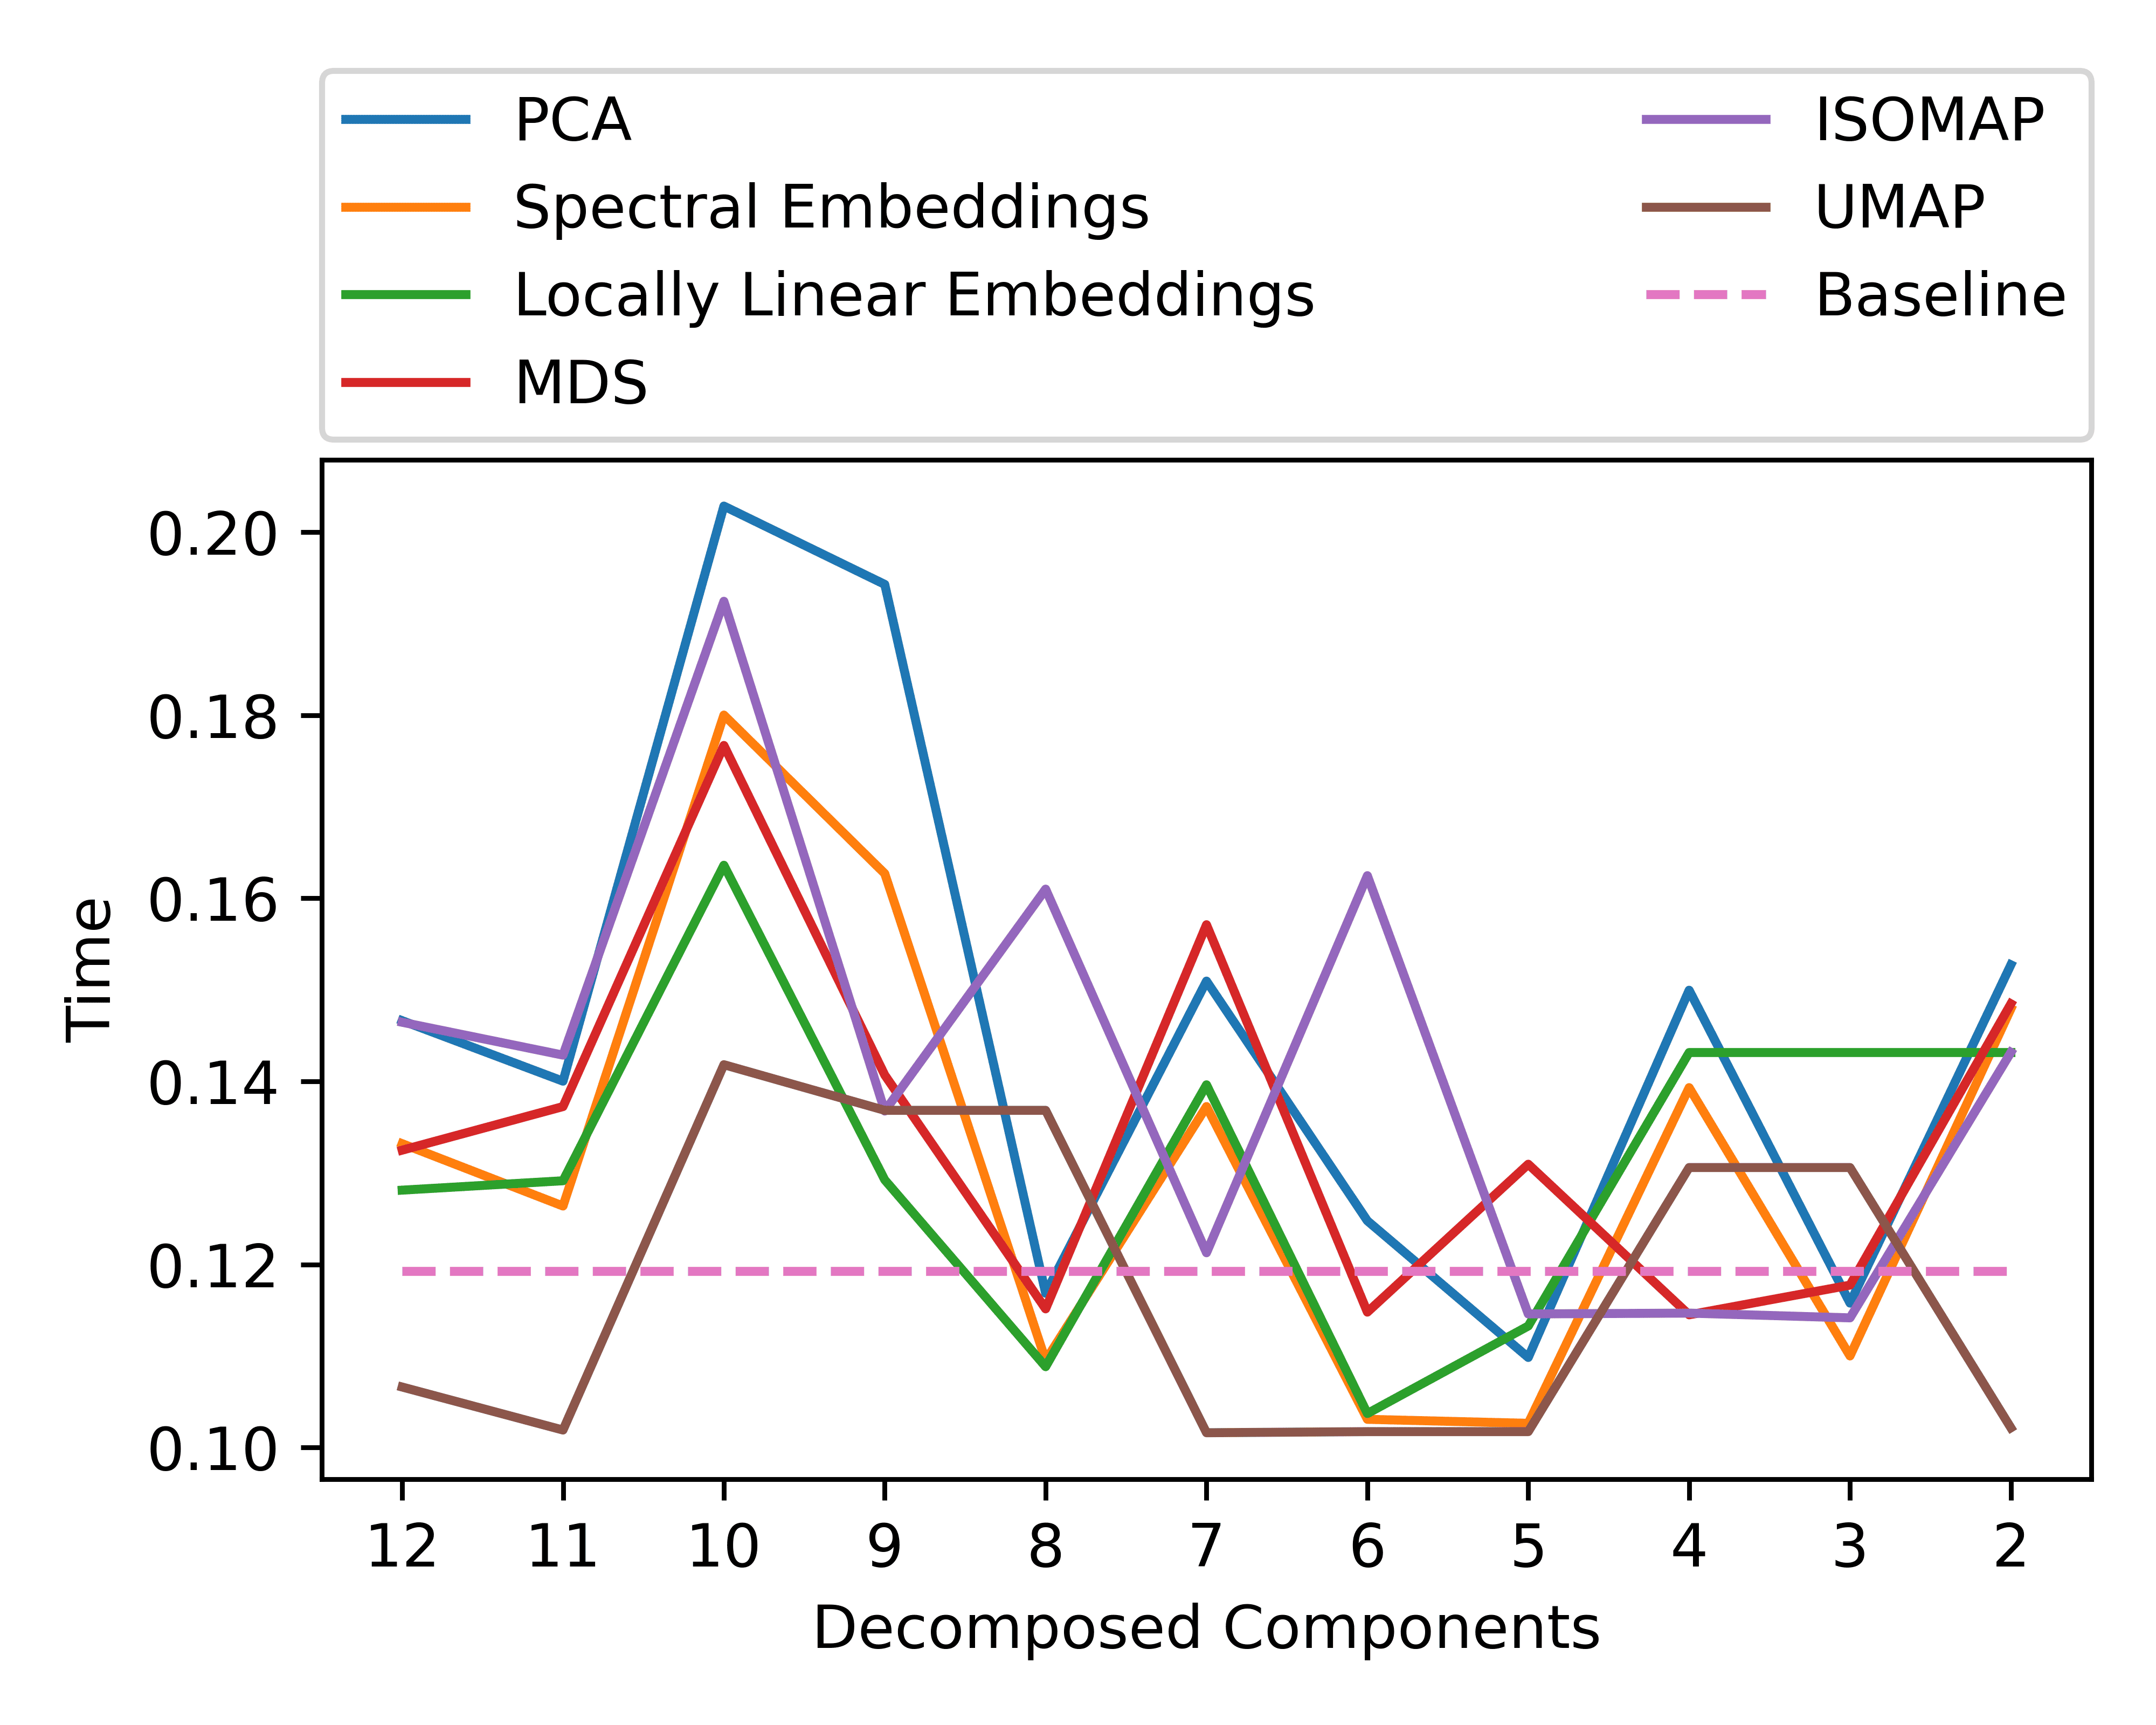
\includegraphics[width=0.48\linewidth]{images/charts_real/real_data_wine_time.png}
                    \label{subfig:wine:time}
                }
                \caption{Анализ влияния различных методов снижения размерности данных на кластеризацию набора данных Wine. Линия Baseline -- результат работы алгоритма \kmeans{} без предварительного снижения размерности. Результаты для
                    \subref{subfig:wine:ami} AMI;
                    \subref{subfig:wine:ari} ARI;
                    \subref{subfig:wine:nmi} NMI, а также на время работы алгоритма \subref{subfig:wine:time}.
                }
                \label{fig:wine}
            \end{figure}

            \begin{figure}[H]\centering
                \includegraphics[width=0.99\linewidth]{images/decomposer/wine_decomposer_analysis.png}
                \caption{Визуализация набора данных Wine после снижения размерности до 2 с использованием PCA, Spectral Embeddings, Locally Linear Embeddings, MDS, ISOMAP, UMAP.}
                \label{fig:wine:example}
            \end{figure}

            На рисунке \ref{fig:wine} представлены результаты экспериментов по кластеризации с предварительным снижением размерности на наборе данных Wine.
            Анализ показал, что методы PCA, ISOMAP и UMAP обеспечивают устойчивое поведение метрик, оставаясь на уровне или вблизи базовой линии на всем диапазоне компонент. Однако, несмотря на эту стабильность, они не продемонстрировали прироста качества кластеризации при уменьшении размерности. В то же время, методы Locally Linear Embeddings (LLE) и Spectral Embeddings показали заметное улучшение показателей AMI, ARI и NMI при переходе к малым числам компонент. Значительный прирост качества заметен у метода Spectral Embeddings, достигающий пика на 2-х компонентах, и опережающий качество исходной кластеризации. Это указывает на его способность извлекать более информативную структуру данных в условиях значительного снижения размерности.


    % \section{Заключение}
    В работе предлагается подход предварительного снижения размерности перед проведением процесса кластеризации \kmeans{}. Было проведено комплексное исследование влияния методов снижения размерности PCA, Spectral Embeddings, Locally Linear Embeddings, MDS, ISOMAP, UMAP на качество кластеризации алгоритмом  \kmeans{}. Основной акцент был сделан на анализ того, как различные подходы к уменьшению размерности данных сохраняют или искажают кластерную структуру, а также как это сказывается на эффективности последующей кластеризации. В результате, было обнаружено, что применение PCA и ISOMAP на синтетических и реальных данных не приводило к снижению качества при переходе в меньшую размерность, при этом на наборе данных Digits метод ISOMAP позволил повысить качество кластеризации более чем на 10\%.
    Код проекта доступен по ссылке \url{www.github.com/alexgiving/LKMeans}.

    \paragraph{Применение суперкомпьютерного комплекса CHARISMA.}
        Исследование выполнено с использованием суперкомпьютерного комплекса НИУ ВШЭ CHARISMA \cite{charisma}.

    \paragraph{Описание применения генеративной модели.}
        В выпускной квалификационной работе использовалась генеративная модель DeepSeek-V3 Chat \cite{deepseekai2024deepseekv3technicalreport}, доступная по ссылке \url{www.deepseek.com}.
        Модель была применена для систематизации и первичного структурирования обзора литературы, что позволило выделить ключевые направления исследований и логично выстроить анализ научных источников. Кроме того, модель использовалась для оформления \LaTeX{} шаблона работы в соответствии с требованиями НИУ ВШЭ, включая корректное применение стилей, разметки и форматирования. Все сгенерированные фрагменты были переработаны и проверены автором вручную. Итоговый текст работы представляет собой результат анализа, интерпретации и авторского изложения материала.



% Include references
\addcontentsline{toc}{section}{Список литературы}
\nocite{*}
\bibliographystyle{ref/IEEEannot}
% \bibliography{ref/annot}
\end{document}